\setcounter{excounter}{1}
\setcounter{examplecounter}{1}
\chapter{Object-Oriented Programming}
\label{chapter-classes} % Always give a unique label
% use \chaptermark{}
% to alter or adjust the chapter heading in the running head

\abstract*{This chapter is divided into two halves. In the first half, we begin to introduce the basics of object-oriented programming. We start off simple with small classes that contain only immutable fields. The complexity gradually increases as we mix in mutability and aliasing. This chapter also describes the implementation of several data structures that mimic those from the Collections framework, including \ttt{ArrayList}, \ttt{LinkedList}, \ttt{HashSet}, and maps.
\\
In the second half, we expand on the details of object-oriented programming by describing interfaces and inheritance. Interfaces ascribe behaviors and characteristics to classes, whereas inheritance denotes ``IS-A'' relationships across classes. We conclude the chapter by demoing a practical application of object-oriented programming and class design by writing a small programming language.}

\abstract{This chapter is divided into two halves. In the first half, we begin to introduce the basics of object-oriented programming. We start off simple with small classes that contain only immutable fields. The complexity gradually increases as we mix in mutability and aliasing. This chapter also describes the implementation of several data structures that mimic those from the Collections framework, including \ttt{ArrayList}, \ttt{LinkedList}, \ttt{HashSet}, and maps.
\\
In the second half, we expand on the details of object-oriented programming by describing interfaces and inheritance. Interfaces ascribe behaviors and characteristics to classes, whereas inheritance denotes ``IS-A'' relationships across classes. We conclude the chapter by demoing a practical application of object-oriented programming and class design by writing a small programming language.}

\section{Classes}
From the first page, we have made prolific use of classes, but in this section we will finally venture into the inner workings of a class, and how to create our own.

\emph{Classes}\index{classes}\index{class} are blueprints for \emph{objects}\index{object}. When we create a class, we declare a new type of object. We encapsulate data and methods inside class definitions for later usage.

As we stated, we have repeatedly used classes, e.g., strings, arrays, \ttt{Scanner}, \ttt{Random}, as well as those classes from the Collections API. Until now, however, we viewed these as forms of abstraction, whose details were not important. 

To create a class, we use the \ttt{class} keyword, followed by the name of the class. The name of the class should be capitalized, and should, in general, describe a noun. All Java files describe a class and must be named accordingly. We, of course, have seen this repeatedly before, but we omitted the details.

Classes can \emph{inherit} methods from other classes, a relationship called the superclass/subclass hierarchy. For now we will only mention that the \ttt{Object} class is the ``ultimate'' superclass, in which all classes are implicit subclasses. The \ttt{Object} class, in particular, has three methods that we will override in almost every class that we write: \ttt{equals}, for comparing two classes for equality, \ttt{toString}, a means of ``stringifying'' an object, and a third: \ttt{hashCode}, the significance of which we will return to soon. In subsequent chapters we will dive more into inheritance and hierarchies.

\myexample{Let's create a class called \ttt{Point}, which stores two \ttt{int} values representing a Cartesian coordinate $x$ and $y$. By ``store,'' we mean to say that $x$ and $y$ are \emph{instance variables}\index{instance variables} of the \ttt{Point} class, also sometimes called \emph{attributes}, \emph{fields}, or \emph{members} (in Java, we conventionally use the ``instance variables'' term). Instance variables denote the values associated with an arbitrary \emph{instance} of that object (an instance may also be defined as an entity). For example, if we have a \ttt{Point} object \ttt{p}, then \ttt{p} has two instance variables, \ttt{x} and \ttt{y}, which are the $x$ and $y$ coordinates of \ttt{p}. Then, if we declare another point \ttt{p2}, then \ttt{p2} will have its own instance variables \ttt{x} and \ttt{y}, which are independent of \ttt{p}'s instance variables. In almost all circumstances, instance variables of a class should be marked as \ttt{private}. Instance variables that are \ttt{private} denotes that direct access to their values is granted only within the class definition. Lastly, for the time being, instance variables are immutable and cannot change. Thus, every instance variable will use the \ttt{final} keyword in its declaration, alongside the \ttt{UPPER\_CASE} naming convention.}

Speaking of \emph{access modifiers}\index{access modifier}, we should mention the four that Java provides, even though we make prolific use of only three:

\begin{itemize}
  \item A class, variable, or method declared with the \ttt{public} modifier is accessible to/by any other class. Variables that are \ttt{public} should be used sparingly.
  \item A class, variable, or method declared with the \ttt{private} modifier is accessible only to/by the class in which it is declared. 
  \item A class, variable, or method declared without an access modifier, also called the \emph{default access modifier}, behaves similarly to \ttt{public}, only that it is accessible only to/by classes in the same package. Packages are a means of organizing classes into groups, similar to directories.
\end{itemize}

The fourth and final access modifier is \ttt{protected}, which is similar to the default access modifier, but allows subclasses to access the variable or method.\footnote{If you have not heard of inheritance/subclasses yet, do not worry, as we will cover this in the next chapter; we explain it here to describe the relevant difference between the access modifiers.} We will not use \ttt{protected} in this text, but it is worth mentioning. As a corollary of sorts, any time that \ttt{protected} \emph{can} be used, there is almost certainly a better design alternative, whether that means marking the variable/method as \ttt{private} or \ttt{public}, we are of the opinion that \ttt{protected} has few benefits. Moreover, because we will not use \ttt{protected}, the use of \ttt{public} will be infrequent and only when necessary.\footnote{Some methods, as we will soon see and have seen previously, are required to be \ttt{public}. For example, the \ttt{main} method must be marked as \ttt{public}.}

\begin{lstlisting}[language=MyJava]
class Point {

  private final int X;
  private final int Y;
}
\end{lstlisting}

We now want a way to create an instance of a \ttt{Point}. We declare instances of objects using the \ttt{new} keyword followed by the class constructor. \emph{Constructors}\index{constructor} are special methods that are called when we wish to create a new object of that class. Our \ttt{Point} class constructor can receive parameters, which we can use to initialize the relevant $x$ and $y$ instance variables. So, let's declare the constructor for our \ttt{Point} class. Constructors, in general, should be \ttt{non-private}, as we will need to call them from outside the class definition. On a case-by-case basis, this changes accordingly, as some classes are local to another class definition and are thereby private. Constructors are also special in that they do not have a return type, although phrasing it in this way leads to some confusion, because constructors have implicit return types. By implicit, we mean that we do not directly specify the return type, but Java knows that constructors are special, whose return types are of the class itself. We create a constructor by specifying the class name alongside any desired parameters.

\begin{lstlisting}[language=MyJava]
class Point {
  
  private final int X;
  private final int Y;
  
  Point(int x, int y) {
    this.X = x;
    this.Y = y;
  }
}
\end{lstlisting}
Remember that the purpose of the constructor is to initialize the class instance variables. So, unless we wish to use distinct identifiers for referencing the parameters and instance variables, we need to use the \ttt{this} keyword.\footnote{Some software engineers and projects use identifier prefixes to refer to instance variables.} The \ttt{this} keyword refers to the current object, and aids in distinguishing between instance variables and parameters. Inside the constructor, we assign the value of the parameter \ttt{x} to the instance variable \ttt{x}. Should we opt to not use \ttt{this} on the left-hand variable identifier, then the parameter \ttt{x} would shadow the instance variable \ttt{x}, meaning that writing \ttt{x = x} assigns the parameter to itself. At last, we can create a \ttt{Point} object by calling the constructor, but wait, we have no way of accessing/referring to the instance variables of the \ttt{Point} object! We need to create \emph{accessor methods}\index{accessor method} to retrieve the values of the instance variables. Accessor methods are non-private and should do exactly one thing: return the respective instance variable.

\begin{lstlisting}[language=MyJava]
class Point {

  private final int X;
  private final int Y;
  
  Point(int x, int y) {
    this.X = x;
    this.Y = y;
  }
  
  int getX() { return this.X; }
  
  int getY() { return this.Y; }
}
\end{lstlisting}

This principle of hiding the implementation details of a class is called \emph{encapsulation}\index{encapsulation}. Encapsulation is a key principle of object-oriented programming, and is one of the primary reasons why object-oriented programming is so powerful. It can be dangerous to directly modify or access the fields of an object.\footnote{By ``dangerous,'' we mean to suggest that it is prone to logic errors.} 

Creating an instance of the \ttt{Point} class is identical to creating an instance of any other arbitrary class. Though, we should first explain a slight terminology distinction.

Declaring, or initializing, an object refers to typing the class name followed by the variable name. For instance, the following code declares a \ttt{Point} object \ttt{p}.

\begin{verbnobox}[\small]
Point p;
\end{verbnobox}

By default, $p$ points to \ttt{null}, since we have not yet created an instance of the \ttt{Point} class. We can create an instance of the \ttt{Point} class by invoking its constructor, an action otherwise called \emph{object instantiation}\index{object instantiation}. We use the \ttt{new} keyword and pass the desired $x$ and $y$ coordinates. 

\begin{verbnobox}[\small]
Point p = new Point(3, 4);
\end{verbnobox}

We should write some tests to ensure that our \ttt{Point} class is working as expected. We note that this may seem redundant for such a simple class and the fact that the accessor methods do nothing more than retrieve instance variable values, but it is a good habit for beginning object-oriented programmers.

\begin{lstlisting}[language=MyJava]
import static Assertions.assertAll;
import static Assertions.assertEquals;

class PointTester {
  
  @Test
  void testPoint() {
    Point p = new Point(3, 4);
    assertEquals(3, p.getX());
    assertEquals(4, p.getY());
  }
}
\end{lstlisting}

Of course, testing the accessor methods is a little boring, so let's override the \ttt{toString} method to print a stringified representation of the \ttt{Point} class. Every object in Java has a \ttt{toString} method, which returns a string representation of the object. By default, the \ttt{toString} method returns the class name followed by the object's hashcode. We can override the \ttt{toString} method by declaring a \ttt{public} method with the signature \ttt{public String toString()} (note that this is one instance where \ttt{public} cannot be avoided.) We can then return a string representation of the object. In this case, we will return a string of the form \ttt{"(x=$x$, y=$y$)"}, where $x$ and~$y$ refer to the respecitve instance variables. 

\begin{lstlisting}[language=MyJava]
class Point {
  // ... previous code not shown.

  @Override
  public String toString() {
    return String.format("(x=%d, y=%d)", this.X, this.Y);
  }
}
\end{lstlisting}

Testing the \ttt{toString} method provides more interesting results, since it requires us to not only override the default implementation of \ttt{toString}, but it also ensures that our constructor correctly initializes the instance variables. Because we will refer to $p$ across several methods, we can declare it as an instance variable of our \ttt{PointTester} class so as to reduce the redundant object instantiation.

\begin{lstlisting}[language=MyJava]
import static Assertions.assertAll;
import static Assertions.assertEquals;

class PointTester {

  private final Point P = new Point(3, 4);

  @Test
  void testPointAccessors() {
    assertEquals(3, P.getX());
    assertEquals(4, P.getY());
  }

  @Test
  void testPointToString() {
    assertEquals("(x=3, y=4)", P.toString());
  }
}
\end{lstlisting}

In addition to the \ttt{toString} method, we might also write other methods associated with a \ttt{Point} object. For example, we might want to calculate the distance between two points. We can write a \ttt{public} method that takes a \ttt{Point} object as a parameter and returns the distance between the two points, the first being the \emph{implicit parameter}, and the second being the \emph{explicit parameter}. We say the first is \emph{implicit} because, under the hood, all class methods take an implicit parameter, which is the object on which the method is called, which is accessible through \ttt{this}. We say the second is \emph{explicit} because we explicitly pass the object as a parameter. 

This is also a good time to bring up another terminology distinction. Some programming languages use \emph{functions}, others use \emph{procedures}, \emph{subroutines}, or \emph{methods}. Going from simplest to most complex, subroutines are simply a sequence of instructions that are executed in order. Procedures are subroutines that return a value. Functions are procedures that take parameters. Methods are functions that are associated with a class. In Java, we use the term \emph{method} to refer to all of these, since all methods must be associated with a class. A language like C++, on the other hand, distinguishes between the two: \emph{functions} refer to subroutines, procedures, or parameter-receiving procedures that are not associated with a class; \emph{methods} are subroutines, procedures, or functions embedded inside a class definition.

Returning to the \ttt{Point} class, we will now write \ttt{distance}, which receives a \ttt{Point} as a parameter and returns the Euclidean distance from \ttt{this} to the parameter. Before doing so, however, we should write a few tests. Conveniently, the three points that we test all have a distance of five between each other.

\begin{lstlisting}[language=MyJava]
import static Assertions.assertAll;
import static Assertions.assertEquals;

class PointTester {

  private static final double DELTA = 0.01;

  private final Point P1 = new Point(3, 4);
  private final Point P2 = new Point(6, 8);
  private final Point P3 = new Point(0, 0);

  @Test
  void testPointDistance() {
    assertAll(
      () -> assertEquals(5, P1.distance(P2), DELTA),
      () -> assertEquals(5, p2.distance(P1), DELTA),
      () -> assertEquals(5, P1.distance(P3), DELTA),
      () -> assertEquals(5, P3.distance(P1), DELTA),
      () -> assertEquals(5, P2.distance(P3), DELTA),
      () -> assertEquals(5, P3.distance(P2), DELTA));
  }
}
\end{lstlisting}

\begin{lstlisting}[language=MyJava]
class Point {
  // ... previous code not shown.

  /**
   * Determines the Euclidean distance between two points.
   * @param p - the other point.
   * @return the distance between this point and p.
   */
  double distance(Point p) {
    int dx = this.X - p.X;
    int dy = this.Y - p.Y;
    return Math.sqrt(dx * dx + dy * dy);
  }
}
\end{lstlisting}

The \ttt{distance} method is called an \emph{instance method} because it is associated with an instance of the class. We can also write \emph{static methods}, which are not associated with an object, but rather the class as a whole. Static methods are declared using the \ttt{static} keyword. Static methods are useful for utility methods that are not associated with a particular instance of the class. All methods designed up until this chapter were static methods, which were not associated with the class in which they resided.

\subsubsection*{Method Overloading}
A method is identified by two attributes: its name, and its signature. Java allows us to \emph{overload}\index{method overloading} a method or constructor by using the same identifier but different parameters.

\myexample{Let's overload the \ttt{distance} method by writing a version that does not receive a parameter at all, and instead returns the magnitude/distance from the point to the origin. Fortunately this is extremely easy, because we can make use of the existing \ttt{distance} method that does receive a \ttt{Point}; we can pass it the origin point, namely \ttt{new Point(0, 0)}, and everything works out wonderfully! Because this version of \ttt{distance} simply refers to the existing definition, which we have thoroughly tested, we will omit a separate tester.}

\begin{lstlisting}[language=MyJava]
class Point {
  // Previous code not shown.
  
  /**
   * Computes the distance from this point to the origin,
   * i.e., (0, 0).
   * @return returns the magnitude of this distance.
   */
   double distance() {
     return this.distance(new Point(0, 0));
   }
}
\end{lstlisting} 

We could, if desired, overload the \ttt{Point} constructor as well. Though, it makes little sense to do so in this specific instance, since a point is defined by its two coordinate members. In subsequent sections, however, we will overload the constructor and demonstrate its utility/practicality.

\myexample{Let's design the static \ttt{averageDistance} method, which receives a \ttt{List<Point>} and computes the average distance away from the origin. We already have a method to compute the distance of a point to the origin, so let's take advantage of the stream API to map \ttt{distance} to every point, then find the average of those resulting double values. This method will return an \ttt{OptionalDouble} in the event that the provided list is empty, which serves as a wrapper around the \ttt{Optional<Double>} type.}

\begin{lstlisting}[language=MyJava]
import static Assertions.assertAll;
import static Assertions.assertEquals;

import java.util.List;
import java.util.Optional;
import java.util.OptionalDouble;

class PointTester {
  // ... previous code not shown.

  @Test
  void testAverageDistance() {
    List<Point> lop = List.of(
            new Point(4, 0), new Point(0, 4),
            new Point(-4, 0), new Point(0, -4),
            new Point(2, 2), new Point(-2, 2),
            new Point(-2, -2), new Point(2, -2));
    assertAll(
      () -> assertEquals(3.414, Point.averageDistance(lop).get(), 0.01),
      () -> assertEquals(OptionalDouble.empty(), Point.averageDistance(List.of())));
  }
}
\end{lstlisting}

\begin{lstlisting}[language=MyJava]
import java.util.List;
import java.util.OptionalDouble;

class Point {
  // ... previous code not shown. 

  /**
   * Computes the average distance to the origin of a list of points.
   * @param lop - list of points.
   * @return empty Optional if the list is empty, or OptionalDouble otherwise.
   */
  static OptionalDouble averageDistance(List<Point> lop) {
    return lop.stream()
              .map(p -> p.distance())
              .mapToDouble(d -> d)
              .average();
  }
}
\end{lstlisting}

\myexample{Let's create the static \ttt{random} method, which returns a \ttt{Point} object with random $x$ and $y$ coordinates. We will use the \ttt{Random} class to generate a random radius and angle as a polar coordinate. Then, we will convert the polar coordinate to Cartesian coordinates. Let's also add a parameter that specifies the maximum radius.}

Because the \ttt{random} method generates a random point, we cannot reasonably write a test that asserts the exact location of the point without prior knowledge of the random seed. Instead, we can write a test that asserts that the point is within a certain radius of the origin. 

\begin{lstlisting}[language=MyJava]
import static Assertions.assertAll;
import static Assertions.assertTrue;

class PointTester {

  @Test
  void testPointRandom() {
    assertAll(
      () -> assertTrue(Point.random(10).distance() <= 10);
      () -> assertTrue(Point.random(1).distance() <= 1);
      () -> assertTrue(Point.random(5).distance() <= 5);
      () -> assertTrue(Point.random(5000000).distance() <= 5000000));
  }
}
\end{lstlisting}

\begin{lstlisting}[language=MyJava]
import java.util.Random;

class Point {

  /**
   * Generates a random point with a maximum radius.
   * @param maxRadius - the maximum radius.
   * @return a random point.
   */
  static Point random(double maxRadius) {
    Random r = new Random();
    double radius = r.nextDouble(maxRadius);
    double angle = r.nextDouble() * Math.PI * 2;
    int x = (int) (radius * Math.cos(angle));
    int y = (int) (radius * Math.sin(angle));
    return new Point(x, y);
  }
}
\end{lstlisting}

We have seen static methods, but what about static variables? A static variable, as we mentioned before, is a variable that is associated with the class and not a specific instance thereof. We can declare a static variable using the \ttt{static} keyword. Static variables are useful for storing information that is shared across all instances of the class. Static variables may be either \ttt{private} or non-\ttt{private}, depending on whether we want to allow direct access to the variable. As with instance variables, however, be wary of granting direct access, since it may lead to logic errors.

\myexample{Suppose we want to keep track of how many instances of \ttt{Point} have been instantiated. Since this is a property of the \ttt{Point} class rather than an instance of the class, we can declare a static variable \ttt{count} to keep track of the number of instances, which is incremented inside the constructor. To remain consistent with our recurring theme of encapsulation, \ttt{count} will be declared as \ttt{private}, and we will write a static method \ttt{getCount} to retrieve the number of instances, which is invoked on the class.\footnote{It is possible to invoke a static method on an instance of the class, but it is considered bad practice and unnecessary.} When testing, we need to be careful to only instantiate instances of \ttt{Point} when we are ready to check the status of \ttt{count}, since the static \ttt{count} variable is incremented inside the constructor.}

\begin{lstlisting}[language=MyJava]
import static Assertions.assertAll;
import static Assertions.assertEquals;

class PointTester {

  @Test
  void testPointCount() {
    assertEquals(0, Point.getCount())
    Point p1 = new Point(3, 4);
    assertEquals(1, Point.getCount());
    Point p2 = new Point(6, 8);
    assertEquals(2, Point.getCount());
    Point p3 = new Point(0, 0);
    assertEquals(3, Point.getCount());

    // Even though we lose reference to p, the static varible still increments!
    for (int i = 0; i < 10; i++) {
      Point p = new Point();
    }
    assertEquals(13, Point.getCount());
  }
}
\end{lstlisting}

\begin{lstlisting}[language=MyJava]
class Point {

  private static int count = 0;

  private final int X;
  private final int Y;

  Point(int x, int y) { this.X = x; this.Y = y; count++; }

  static int getCount() { return count; }
}
\end{lstlisting}

Notice that, inside the \ttt{getCount} method, we do not refer to \ttt{count} with \ttt{this}, since \ttt{count} is a static variable and not an instance variable. Prefixing the \ttt{count} variable with \ttt{this} results in a compiler error. Further note that the variable is not marked as \ttt{final}, since it is not immutable and changes with every newly-instantiated \ttt{Point} object.

\myexample{Imagine we want to store a collection of \ttt{Point} objects in a data structure such as a \ttt{HashSet}. The question that arises from this decision is apparent: how do we determine if a \ttt{Point} is already inside the set? We need to override two important methods from \ttt{Object}: \ttt{public boolean equals} and \ttt{public int hashCode}. The \ttt{equals} method of an object determines how we wish to compare two instances of the class. In this circumstance, let's say that two points are equal according to \ttt{equals} if and only if they share the same $x$ and $y$ coordinates. Overriding the \ttt{equals} method from the \ttt{Object} class requires correctly copying the signature, the sole parameter being an \ttt{Object} that we want to check for type equality. In other words, we first want to verify that the passed object to the \ttt{equals} method is, in fact, a \ttt{Point}, otherwise they cannot possibly be equal. We can use the \ttt{instanceof} operator to our advantage. From here, if the input parameter is a \ttt{Point}, we can cast the parameter to a \ttt{Point}, then check whether or not the coordinates match. Moreover, like \ttt{toString}, the \ttt{equals} and \ttt{hashCode} methods are definitionally \ttt{public}, so do not forget the access modifier.}

\begin{lstlisting}[language=MyJava]
import static Assertions.assertAll;
import static Assertions.assertEquals;
import static Assertions.assertNotEquals;

class PointTester {

  @Test
  void testEquals() {
    assertAll(
      () -> assertEquals(new Point(3, 3), new Point(3, 3)),
      () -> assertNotEquals(new Point(3, 4), new Point(3, 7)),
      () -> assertNotEquals(new Point(7, 4), new Point(10, 4)),
      () -> assertNotEquals(new Point(10, 30), new Point(3, 7)));
  }
}
\end{lstlisting}

\begin{lstlisting}[language=MyJava]
class Point {
  // ... previous code not shown.

  @Override
  public boolean equals(Object obj) {
    if (!(obj instanceof Point)) { return false; }
    else {
      Point othPt = (Point) obj;
      return this.x == othPt.x && this.y == othPt.y;
    }
  }
}
\end{lstlisting}

Let's try to create an instance of a \ttt{HashSet}, then iterate over the elements of the set after adding two of the same \ttt{Point} instances, i.e., points that share coordinates. Doing so demonstrates a glaring flaw: the set appears to have added both \ttt{Point} instances to the set despite their sharing of coordinates! The reason is incredibly subtle and easy to miss: the \ttt{Object} class invariant states that, if two objects are equal according to \ttt{equals}, then their hashcodes must also be equal. The hashcode of an object is simply an integer used for quick access/lookup in hashable data structures such as \ttt{HashSet} and \ttt{HashMap}. Indeed, the problem is that we forgot to override \ttt{hashCode} after overriding the \ttt{equals} method. Bloch~\cite{effectivejava} states, as a principle, that whenever we override \ttt{equals}, we should accompanyingly override the \ttt{hashCode} implementation. Now, you might wonder: ``How can I hash an object?'' Fortunately Java has a method in the \ttt{Objects} class called \ttt{hash}, which receives any number of arguments and runs them through a hashing algorithm, thereby returning the hash of the parameters. When overriding \ttt{hashCode} we should include all instance variables of the object to designate that all of the properties affect the object's hashcode. After fixing the issue, we see that our \ttt{HashSet} now correctly contains only one of the \ttt{Point} objects that we add.

\begin{lstlisting}[language=MyJava]
import static Assertions.assertTrue;

import java.util.Set;
import java.util.HashSet;

class PointTester {

  @Test
  void testHashSetPoint() {
    Set<Point> p = new HashSet<>();
    p.add(new Point(3, 3));
    p.add(new Point(3, 3));
    assertTrue(p.size() == 1);
  }
}
\end{lstlisting}

\begin{lstlisting}[language=MyJava]
import java.util.Objects;

class Point {
  // ... previous code not shown.

  @Override
  public int hashCode() {
    return Objects.hash(this.x, this.y);
  }
}
\end{lstlisting}

\myexample{Let's design the static \ttt{removeLinearPoints(List<Point> lop)} method that, when given a \ttt{List<Point>}, filters out all points that are ``linear,'' meaning that they share an $x$ and $y$ coordinate. Fortunately, as with the previous example, streams make this exercise a walk in the park. Because we overrode the \ttt{equals} definition, the comparisons by \ttt{assertEquals} will work correctly. That is, we are comparing the elements of two lists of \ttt{Point} objects. The \ttt{assertEquals} method uses the object's \ttt{.equals} method implementation for object equivalence comparisons, meaning that it will check each element of both lists to determine if they are all equivalent.}

\begin{lstlisting}[language=MyJava]
import static Assertions.assertAll;
import static Assertions.assertEquals;

import java.util.List;

class PointTester {
  // ... previous code not shown. 

  @Test
  void testRemoveLinearPoints() {
    List<Point> lop = List.of(new Point(5, 10), new Point(7, 7),
                              new Point(2, 3), new Point(4, 3),
                              new Point(1, 1), new Point(-6, -10),
                              new Point(-23, -23), new Point(1, 0));
    List<Point> lopRes = List.of(new Point(5, 10), new Point(2, 3),
                                 new Point(4, 3), new Point(-6, -10),
                                 new Point(1, 0));
    assertAll(
      () -> assertEquals(List.of(), Point.removeLinearPoints(List.of())),
      () -> assertEquals(lopRes, Point.removeLinearPoints(lop)));
  }
}
\end{lstlisting}

\begin{lstlisting}[language=MyJava]
import java.util.List;

class Point {
  // ... previous code not shown. 

  /**
   * Returns a list of all points that are not "linear."
   * @param lop - list of Point objects.
   * @return list where linear points are removed.
   */
  static List<Point> removeLinearPoints(List<Point> lop) {
    return lop.stream()
              .filter(p -> p.getX() != p.getY())
              .toList();
  }
}
\end{lstlisting}

\myexample{Let's amplify the complexity a bit by designing a ``21'' card game, which is a card game where the players try to get a card value total of $21$ without going over. We should think about the design process of this game, namely what classes we need to create. It makes sense to start off with a \ttt{Card} class, which stores its suit and its numeric value. Because a suit is one of four possibilities, each of which uses a different symbol, we can create another class called \ttt{Suit}. In \ttt{Suit} we instantiate four static instances of \ttt{Suit}, each of which represents one of the four valid suits. Its constructor is privatized because we, as the programmers, define the four possible suits; it should not be possible for the user to define their own custom suit, at least for this particular game. The notion of \ttt{Suit} being an instance variable of \ttt{Card}, and only exists due to \ttt{Card} is called \emph{object composition}. Lastly, we will provide a method that returns an \ttt{Iterator<Suit>} over the four suit possibilities to make our lives easier when designing the \ttt{Deck} class. The method should be static so it is accessible through the class.}

\begin{lstlisting}[language=MyJava]
class Suit {

  static final Suit CLUBS = new Suit("(*;$\clubsuit$;*)");
  static final Suit DIAMONDS = new Suit("(*;$\diamondsuit$;*)");
  static final Suit HEARTS = new Suit("(*;$\heartsuit$;*)");
  static final Suit SPADES = new Suit("(*;$\spadesuit$;*)");
  static final int NUM_SUITS = 4;

  private final String S_VAL;

  private Suit(String s) { this.S_VAL = s; }

  static Iterator<Suit> iterator() {
    return new ArrayList<Suit>(List.of(CLUBS, DIAMONDS, HEARTS, SPADES))
                              .iterator();
  }

  @Override
  public String toString() { return this.S_VAL; }
}
\end{lstlisting}

Testing the \ttt{Card} class is simple and straightforward; we only need to test one method, the \ttt{toString} method, since testing \ttt{getValue}, at this point, is superfluous. We could also test the \ttt{Suit} class, but we will not do so here, given that the only useful methods are to retrieve the instance variables and the iterator.

\begin{lstlisting}[language=MyJava]
import static Assertions.assertAll;
import static Assertions.assertEquals;

class CardTester {

  @Test
  void testCardToString() {
    assertAll(
      () -> assertEquals("2 of (*;$\clubsuit$;*)", new Card(Suit.CLUBS, 2).toString()),
      () -> assertEquals("3 of (*;$\diamondsuit$;*)", new Card(Suit.DIAMONDS, 3).toString()),
      () -> assertEquals("4 of (*;$\heartsuit$;*)", new Card(Suit.HEARTS, 4).toString()),
      () -> assertEquals("5 of (*;$\spadesuit$;*)", new Card(Suit.SPADES, 5).toString()));
  }
}
\end{lstlisting}

\begin{lstlisting}[language=MyJava]
class Card {

  private final Suit SUIT;
  private final int VAL;

  Card(Suit suit, int value) { this.SUIT = suit; this.VAL = value; }
  
  @Override
  public String toString() { return String.format("%d of %s", this.VAL, this.SUIT); }

  int getValue() { return this.VAL; } 
}
\end{lstlisting}

In a standard fifty-two deck of cards, some are ``special,'' e.g., the Jacks, Queens, Kings, and Ace cards. To simplify our design, these cards will be treated the same as a ``ten'' card, showing no syntactic nor semantic difference. Now that we have a class to represents cards, let's design the \ttt{Deck} class, which stores an \ttt{ArrayList<Card>} representing the current state of the deck. It also contains a static variable representing the maximum number of allowed cards. For our purposes, as we alluded to, this quantity is fifty-two. In the \ttt{Deck} constructor, we will call the \ttt{populateDeck} method, which adds four cards of the same value, but of each suit. So, to exemplify, this means that there are four cards whose value is three, where each is one of the four suits. We make use of the iterator from the \ttt{Suit} class to simplify our deck population. Only the \ttt{Deck} class needs to know how to populate an initial (empty) deck, so we privatize its implementation.

To test a \ttt{Deck}, we can write a \ttt{drawCard} method, which retrieves the ``top-most'' card on the deck to see if it is in the correct order. According to our implementation of the iterator, the top-most cards should have values of ten and be of the same suit. From there, we can draw three more cards to ensure they are of values nine, eight, and seven of the same suit. The iterator places \ttt{DIAMOND} as the final suit, so this is what we will assume in our tester. It might also be beneficial to test the \ttt{isEmpty} method, which returns \ttt{true} if the deck is empty, and \ttt{false} otherwise. We can test this functionality by drawing all fifty-two cards from the deck and ensuring that the deck is empty afterwards. Note that we draw four tens because there are no ``Kings,'' ``Queens,'' or ``Jacks'' in the deck.

\begin{lstlisting}[language=MyJava]
import static Assertions.assertAll;
import static Assertions.assertEquals;
import static Assertions.assertTrue;
import static Assertions.assertFalse;

class DeckTester {

  @Test
  void testDeckDrawCard() {
    Deck d = new Deck();
    assertAll(
      () -> assertEquals("10 of (*;$\diamondsuit$;*)", d.drawCard().toString()),
      () -> assertEquals("10 of (*;$\diamondsuit$;*)", d.drawCard().toString()),
      () -> assertEquals("10 of (*;$\diamondsuit$;*)", d.drawCard().toString()),
      () -> assertEquals("10 of (*;$\diamondsuit$;*)", d.drawCard().toString()),
      () -> assertEquals("9 of (*;$\diamondsuit$;*)", d.drawCard().toString()));
  }

  @Test
  void testDeckIsEmpty() {
    Deck d = new Deck();
    for (int i = 0; i < 52; i++) {
      assertFalse(d.isEmpty());
      d.drawCard();
    }
    assertTrue(d.isEmpty());
  }
}
\end{lstlisting}

\begin{lstlisting}[language=MyJava]
import java.util.ArrayList;
import java.util.Iterator;

class Deck {

  private static final int MAX_NUM_CARDS = 52;

  private final ArrayList<Card> CARDS;

  Deck() {
    this.CARDS = new ArrayList<Card>();
    this.populateDeck();
  }

 /**
  * Retrieves a card from the "top" of the deck. If the
  * deck is empty, we return null.
  * @return the top-most card in the deck, or null if the deck is empty.
  */
  Card drawCard() {
    return this.CARDS.isEmpty() ? null : this.CARDS.remove(this.CARDS.size() - 1);
  }

  /**
   * Determines if the deck is empty.
   * @return true if the deck contains no cards, and false otherwise.
   */
  boolean isEmpty() { 
    return this.CARDS.isEmpty(); 
  }

  /**
   * Instantiates the deck to contain all 52 cards.
   * Note that the deck contains cards in-order by suit. There are 
   * no face cards in the deck, i.e., no Jack, Queen, King, nor ace.
   * All cards have a value between 1 and 10.
   */
  private void populateDeck() {
    // For every suit, create 13 cards, the last four of which all have
    // a value of ten.
    Iterator<Suit> it = Suit.iterator();
    while (it.hasNext()) {
      Suit s = it.next();
      for (int i = 1; i <= MAX_NUM_CARDS / Suit.NUM_SUITS; i++) {
        Card c = new Card(s, Math.min(10, i));
        this.CARDS.add(c);
      }
    }
  }
}
\end{lstlisting}

Hopefully the \ttt{populateDeck} method is intuitive and not intimidating. All we do is create fifty two cards, thirteen of which are of the same suit, and add them to the deck. We use the \ttt{Math.min} method to ensure that the value of the card is at most ten, since we do not have ``King,'' ``Queen,'' or ``Jack'' cards. We also use the ternary operator to check if the deck is empty before drawing a card. If the deck is empty, we return \ttt{null}.

Finally we come to the \ttt{Player} class, which stores a ``hand'' containing the cards in their possession. Fortunately this is a very straightforward definition and contains four one-line methods: \ttt{addCard}, \ttt{clearHand}, \ttt{getScore}, and \ttt{toString}. The former two are trivial to explain, as is \ttt{toString}, whereas \ttt{getScore} is the only slightly convoluted method. The idea is to return an integer that represents the total value of the cards in the player's hand. Since streams were introduced a couple of chapters ago, we will once again use them to our advantage.

\begin{lstlisting}[language=MyJava]
import java.util.ArrayList;

class Player {

  private final ArrayList<Card> HAND;

  Player() { this.HAND = new ArrayList<Card>(); }

  /**
   * Adds a card to the player's hand.
   * @param c - card to add to the player's hand.
   */
  void addCard(Card c) { this.HAND.add(c); }

  /**
   * Removes all cards from the player's hand.
   */
  void clearHand() { this.HAND.clear(); }

  /**
   * Determines the player's score.
   * @return the player's score.
   */
  int getScore() {
    return this.HAND.stream()
                    .map(c -> c.getValue())
                    .reduce(0, Integer::sum);
  }

  @Override
  String toString() {
    return String.format("Score: %d\nHand: %s\n", 
                         this.getScore(), this.HAND.toString());
  }
}
\end{lstlisting}

Using the capabilities of \ttt{Player}, \ttt{Deck}, and \ttt{Card}, we will write \ttt{TwentyOne}: the class that runs a game of ``twenty-one.'' The game logic is simple: if the game is still running, clear the player's hand, create a new deck of cards, shuffle them, and give the player two. Then, ask the player if they want to draw another card. If they do, draw a card and add it to their hand. If they do not, then the game is over. If the player's score is greater than twenty-one, then the player loses. Otherwise, the player wins. We will also write a \ttt{main} method that runs the game. We will not write any tests for this class, since it interacts with the user through the \ttt{Scanner} class.

It should be noted that this version of ``twenty-one'' only has the objective of getting as close as possible to a hand containing cards with a value that sums to twenty one, compared to a more-traditional card game where multiple players exist, with a dealer to distribute cards. As exercises, there are many ways to enhance the game, including adding a ``high score'' board to keep track of previous game outcomes, introducing CPU players to automatically poll cards from the deck to beat the main player, or even adding more human players through standard input/output iteractions. 

\begin{lstlisting}[language=MyJava]
import java.util.Scanner;

class TwentyOne {

  private static final int MAX_SCORE = 21;

  private final Player PLAYER;

  TwentyOne() { this.PLAYER = new Player(); }

  /**
   * Plays a game of "21", where the player has to draw cards until they
   * get as close to 21 as possible without going over.
   */
  void playGame() {
    Scanner in = new Scanner(System.in);
    boolean continuePlaying = true;
    while (continuePlaying) {
      // Clear the player's hand.
      this.player.clearHand();

      // Create and shuffle the deck.
      Deck d = new Deck();
      d.shuffleDeck();

      // First, deal two cards.
      this.PLAYER.addCard(d.drawCard());
      this.PLAYER.addCard(d.drawCard());

      // While the player has not "busted", ask them to draw a card or stand.
      while (this.PLAYER.getScore() <= this.MAX_SCORE) {
        System.out.println(this.PLAYER);
        System.out.println("Do you want to draw? (Y/n)");
        String resp = in.nextLine();
        if (resp.equals("Y")) { this.PLAYER.addCard(d.drawCard()); }
        else { break; }
      }

      // Print the final results of the player.
      System.out.println(this.PLAYER);
      if (this.PLAYER.getScore() > this.MAX_SCORE) {
        System.out.println("You lose!");
      } else {
        System.out.println("You did not go over!");
      }

      // Determine if we're still playing.
      System.out.println("Do you want to continue playing?");
      String resp = in.nextLine();
      continuePlaying = resp.equals("Y");
    }
  }

  public static void main(String[] args) {
    new TwentyOne().playGame();
  }
}
\end{lstlisting}

Designing interactive games is a great exercise in object-oriented programming, as well as the culmination of other discussed topics.

\myexample{Let's design the \ttt{Rational} class, which stores a rational number as a numerator and denominator. In doing so we will create methods for adding, subtracting, multiplying, and dividing rational numbers. Testing is paramount with this example, so we will be sure to write plenty. Recall the definition of a rational number: a number that can be expressed as the ratio of two integers~$p$~and~$q$, namely $p/q$. We are acutely familiar with how to perform basic operations on fractions from grade school, so we will glide through the actual mathematics and focus more on the Java implementation and class design.}

The \ttt{Rational} constructor receives two integers $p$ and $q$, and assigns them as instance variables. The \ttt{toString} method is trivial to write and only involves us adding a slash between our numerator and denominator. Though, let's back up for a second and rethink the constructor. Do we really want to be able to store fractions that are not in their simplest form? For example, do we want to allow the user to create a \ttt{Rational} object with a numerator of $2$ and a denominator of $4$? The answer is probably not, meaning that we should add a method that simplifies the fraction. We can do this by finding the greatest common divisor of the numerator and denominator, and dividing both by that value. Euclid's algorithm for finding the greatest common divisor of two integers works wonderfully here. Due to its trivial implementation and the fact that it is a tail recursive algorithm exercise from the previous chapters, we will omit its implementation.

\begin{lstlisting}[language=MyJava]
import static Assertions.assertAll;
import static Assertions.assertEquals;

class RationalTester {
  
  @Test
  void testRationalToString() {
    assertAll(
      () -> assertEquals("1/2", new Rational(1, 2).toString()),
      () -> assertEquals("3/400", new Rational(3, 400).toString()),
      () -> assertEquals("1/1305", new Rational(5, 6525).toString()),
      () -> assertEquals("3591/46562", new Rational(7182, 93124).toString()),
      () -> assertEquals("7/32", new Rational(7, 32).toString()),
      () -> assertEquals("9388/48122", new Rational("4694/24061").toString()),
      () -> assertEquals("1/1", new Rational(1, 1).toString()));
  }
}
\end{lstlisting}

\begin{lstlisting}[language=MyJava]
class Rational {
  
  private final long NUMERATOR;
  private final long DENOMINATOR;

  Rational(long numerator, long denominator) {
    long gcd = gcd(numerator, denominator);
    this.NUMERATOR = numerator / gcd;
    this.DENOMINATOR = denominator / gcd; 
  }

  @Override
  public String toString() {
    return String.format("%ld/%ld", this.NUMERATOR, this.DENOMINATOR);
  }
}
\end{lstlisting}

To add two rational numbers $r_1$ and $r_2$, they must share a denominator. If they do not, then we must find a common denominator by multiplying the denominators together, then multiplying the relevant numerators by the reciprocals of the denominator. For instance, if we want to add $2/3$ and $7/9$, the (not-necessarily lowest) common denominator is $3\cdot{9} = 27$. We then multiply $2$ by $9$ and $7$ by $3$ to get $18/27$ and $24/27$. Adding across the numerators results in $42/27$, which reduces to $14/9$. Since we wish to preserve the original rational number, we will write a method that returns a new \ttt{Rational} rather than modifying the one we have in-place (this also allows us to omit a step in which we simplify the resulting fraction, since the constructor takes care of this task).

\begin{lstlisting}[language=MyJava]
import static Assertions.assertAll;
import static Assertions.assertEquals;

class RationalTester {

  @Test
  void testRationalAdd() {
    assertAll (
      () -> assertEquals("14/9", 
                         new Rational(2, 3).add(new Rational(7, 9)).toString()),
      () -> assertEquals("5/6", 
                         new Rational(1, 2).add(new Rational(1, 3)).toString()),
      () -> assertEquals("1/3", 
                         new Rational(1, 4).add(new Rational(1, 12)).toString()),
      () -> assertEquals("1/4", 
                         new Rational(1, 8).add(new Rational(1, 8)).toString()),
      () -> assertEquals("1/8", 
                         new Rational(1, 16).add(new Rational(1, 16)).toString()),
      () -> assertEquals("1/16", 
                         new Rational(1, 32).add(new Rational(1, 32)).toString()),
      () -> assertEquals("2/1", 
                         new Rational(32, 32).add(new Rational(32, 32)).toString()));
  }
}
\end{lstlisting}

\begin{lstlisting}[language=MyJava]
class Rational {
  // Other details not shown.

  /**
   * Adds two rational numbers.
   * @param r - the other rational number.
   * @return the (simplified) sum of this and r.
   */
  Rational add(Rational r) {
    long commonDenominator = this.DENOMINATOR * r.DENOMINATOR;
    long newNumerator = this.NUMERATOR * r.DENOMINATOR 
                        + r.NUMERATOR * this.DENOMINATOR;
    return new Rational(newNumerator, commonDenominator);
  }
}
\end{lstlisting}

Due to the correspondence to addition, we will leave \ttt{subtraction} as an exercise to the reader. We can now do multiplication, which is even simpler than addition; all that is needed is to multiply the numerators and denominators together. We will also leave \ttt{division} as an exercise to the reader. We also encourage the reader to write methods for comparing rationals for equality, as well as greater than/less than. Plus, we could extend this system to support \ttt{BigInteger} values for the numerator and denominator, which would allow us to represent arbitrarily large rational numbers. This, in turn, would require updating all methods to use \ttt{BigInteger} arithmetic, which is a good exercise in itself.

\begin{lstlisting}[language=MyJava]
import static Assertions.assertAll;
import static Assertions.assertEquals;

class RationalTester {

  @Test
  void testRationalMultiply() {
    assertAll (
      () -> assertEquals("14/27", 
                         new Rational(2, 3).multiply(new Rational(7, 9)).toString()),
      () -> assertEquals("1/6", 
                         new Rational(1, 2).multiply(new Rational(1, 3)).toString()),
      () -> assertEquals("1/48", 
                         new Rational(1, 4).multiply(new Rational(1, 12)).toString()),
      () -> assertEquals("1/64", 
                         new Rational(1, 8).multiply(new Rational(1, 8)).toString()),
      () -> assertEquals("1/25", 
                         new Rational(1, 5).multiply(new Rational(1, 5)).toString()),
      () -> assertEquals("1/1", 
                         new Rational(1, 1).multiply(new Rational(1, 1)).toString()));
  }
}
\end{lstlisting}

\begin{lstlisting}[language=MyJava]
class Rational {
  // ... previous code not shown.

  /**
   * Multiplies two rational numbers.
   * @param r - the other rational number.
   * @return the (simplified) product of this and r.
   */
  Rational multiply(Rational r) {
    return new Rational(this.NUMERATOR * r.NUMERATOR, 
                        this.DENOMINATOR * r.DENOMINATOR);
  }
}
\end{lstlisting}

\myexample{Let's now use classes to demonstrate a theoretically powerful idea: translating standard recursive methods into ones that use iteration. We have seen how to translate a tail recursive method, but standard recursion was left out of the discussion. In general, any recursive method can be rewritten to use iteration. The problem we encounter with standard recursive algorithms is that they often blow up the procedure call stack, of which is very limited in size for most programming languages. What if we did not push anything to the call stack at all, and instead implement our own stack? In doing so, we delegate the space requirements of the recursive calls from the (call) stack to the heap, of which there is orders of magnitude more space. This solution is neither fast nor space-efficient, but serves to show that naturally standard recursive algorithms, e.g., factorial, can still use standard recursion in a sense.}

To create our own stack, we first need to decide what goes inside the stack. We know that each method call pushes an activation record, or a stack frame, to the procedure call stack containing the existing local variables and parameters. For the sake of simplicity, let's assume that our methods never declare local variables. We need a class that stores variable identifiers to values, which can be any type. A simple solution to the ``any type'' problem is to use the \ttt{Object} class that all classes implicitly extend. So, the \ttt{StackFrame} class stores a \ttt{Map<String, Object>} as an instance variable. Its constructor receives no arguments because we do not know a priori how many parameters any arbitrary user of \ttt{StackFrame} will require. To compensate, let's write the \ttt{addParam} method that receives a \ttt{String} and an \ttt{Object}, enters those into the existing map, and returns the existing instance.\footnote{This idea resembles the \emph{builder} design pattern, which we will discuss in Chapter~\ref{chapter-modern}.} We design the method in this fashion to prevent the need to separately instantiate the frame, then add its parameters on separate lines, which would be required if \ttt{addParam} were of type void.

\begin{lstlisting}[language=MyJava]
import java.util.HashMap;
import java.util.Map;

class StackFrame {

  private Map<String, Object> PARAMS;

  StackFrame() { 
    this.PARAMS = new HashMap<>(); 
  }

  Object getParam(String s) { 
    return this.PARAMS.get(s); 
  }

  StackFrame addParam(String s, Object o) {
    this.PARAMS.put(s, o);
    return this;
  }
}
\end{lstlisting}

Now, let's translate the standard recursive \ttt{fact} method, which will receive a \ttt{BigInteger}, and return its factorial. Below we show the recursive version. From this, we write the \ttt{factLoop} method that instantiates a \ttt{Stack<StackFrame>} to replicate the call stack. We begin the process by pushing the initial frame, which stores the initial input argument. This is followed by a variable to keep track of the ``return value,'' which should match the type of the standard recursive method (for our purposes of factorial, this is a \ttt{BigInteger}). Our loop continues as long as there is a stack frame to pop, and the core logic of the algorithm, namely $n!$, is identical to our standard recursive counterpart.

\begin{lstlisting}[language=MyJava]
import static Assertions.assertAll;
import static Assertions.assertEquals;

import java.util.BigInteger;

class StackFrameTester {

  @Test
  void testFact() {
    assertAll (
      () -> assertEquals(new BigInteger("1"), 
                         fact(new BigInteger("0"))),
      () -> assertEquals(new BigInteger("120"), 
                         fact(new BigInteger("5"))),
      () -> assertEquals(new BigInteger("3628800"), 
                         fact(new BigInteger("100"))),
    );
  }

  @Test
  void testFactLoop() {
      assertAll (
      () -> assertEquals(new BigInteger("1"), 
                         factLoop(new BigInteger("0"))),
      () -> assertEquals(new BigInteger("120"), 
                         factLoop(new BigInteger("5"))),
      () -> assertEquals(new BigInteger("3628800"), 
                         factLoop(new BigInteger("100"))),
    );
  }
}  
\end{lstlisting}

\begin{lstlisting}[language=MyJava]
import java.util.Stack;
import java.util.BigInteger;

class StackFrameDriver {

  static BigInteger fact(BigInteger n) {
    if (n.compareTo(BigInteger.ONE) <= 0) {
      return n.add(BigInteger.ONE);
    } else {
      return n.multiply(fact(n.subtract(BigInteger.ONE)));
    }
  }

  static BigInteger factLoop(BigInteger n) {
    Stack<StackFrame> sf = new Stack<>();
    BigInteger res = n;
    sf.push(new StackFrame().addParam("n", n));
    while (!sf.isEmpty()) { /* TODO. */ }
    return res;
  }
}
\end{lstlisting}

Turning our attention to the innards of the loop, we must accurately replicate the procedure call stack actions. Thus, we first pop the existing frame, extract the desired parameters to work with from its map, then perform the algorithm's logic.

\begin{lstlisting}[language=MyJava]
class StackFrameDriver {
  // ... previous code not shown.

  static BigInteger factLoop(BigInteger n) {
    Stack<StackFrame> sf = new Stack<>();
    BigInteger res = BigInteger.ONE;
    sf.push(new StackFrame().addParam("n", n));

    while (!sf.isEmpty()) {
      StackFrame f = sf.pop();
      BigInteger pn = (BigInteger) f.get("n");
      if (pn.compareTo(BigInteger.ONE) <= 0) { continue; }
      else {
        sf.push(new StackFrame().addParam("n", pn.subtract(BigInteger.ONE)));
        res = res.multiply(pn);
      }
    }

    return res;
  }
}
\end{lstlisting}

With this, notice two things: first, we mimic the behavior of the call stack manually. This consequently means that, unless there is a method inside that uses the stack, we never push any activation records. Second, by managing the stack ourselves, we drastically increase the limit to the number of possible ``recursive calls,'' since we push instances of our \ttt{StackFrame} onto the heap. Theoretically, we could continuously push new ``frames'' to our stack so long as we have active and available heap memory. This, of course, is impossible with current hardware limitations, so in due time, with a large-enough call to \ttt{factLoop}, the JVM terminates the program with an \ttt{OutOfMemory} exception. In the relevant test suite, we do not include tests for extraordinarily large numbers to preserve space, but we encourage the readers to try out such test cases, e.g., $100000000!$. We should state that these tests will not complete in a reasonable amount of time.\footnote{On an AMD Ryzen 5 3600 with 16GB of DDR4 RAM, this test did not complete within a three hour time frame.} 
\section{Object Mutation and Aliasing}
\label{sec:object-mutation-and-aliasing}
A limitation that we have purposefully imposed on our object/class design is the inability to modify the values of instance variables. Value mutation is a foreign concept in some programming languages, but we have made extensive use of it throughout our time in the land of Java. In this section, we will discuss the implications of allowing instance variable mutation and how it can lead to some unexpected behavior.

To access a \ttt{private} instance variable, we design a \ttt{public} accessor method, which returns the instance variable. To modify a \ttt{private} instance variable, we design a \ttt{public} mutator method\index{mutator method}\index{setter method}, which takes in a parameter and assigns the instance variable to the parameter. Let's return to the \ttt{Point} class to demonstrate. Suppose that we instantiate a point $p$ to $(7, 4)$, but we then want to change or modify either coordinate. We can do so by calling the \ttt{setX} or \ttt{setY} methods, respectively. Testing setter methods is important to verify that a change occurred when invoking the setter/mutator method, which we confirm through the accessor method. Another way of phrasing this is that, when testing a mutator, we care about the \emph{side-effect}\index{side-effect} of the method rather than what it returns, namely nothing. Setter methods, or methods that modify outside values or data are definitionally \emph{impure}\index{impure}. Because we want to be able to alter an instance variable, these can no longer be marked as \ttt{final}, so we remove this keyword.\footnote{This is not to suggest that we should never use \ttt{final} instance variables. In fact, we \emph{should} use \ttt{final} instance variables whenever possible, since object mutation introduces the possibility of easy-to-overlook bugs.}

%\enlargethispage{1\baselineskip}
\begin{lstlisting}[language=MyJava]
import static Assertions.assertAll;
import static Assertions.assertEquals;

class PointTester {

  @Test
  void testSetX() {
    Point p = new Point(7, 4);
    p.setX(3);
    assertEquals(3, p.getX());
  }

  @Test
  void testSetY() {
    Point p = new Point(7, 4);
    p.setY(2);
    assertEquals(2, p.getY());
  }
}
\end{lstlisting}

\begin{lstlisting}[language=MyJava]
class Point {

  private int x;
  private int y;

  Point(int x, int y) { 
    this.x = x; 
    this.y = y; 
  }

  int getX() { return this.x; }
  int getY() { return this.y; }
  void setX(int x) { this.x = x; }
  void setY(int y) { this.y = y; }
}
\end{lstlisting}

What are some consequences to mutating an object? One comes through the notion of \emph{object aliasing}. Recall that objects point to references in memory. Therefore if we instantiate a \ttt{Point} $p_1$, then initialize another \ttt{Point} $p_2$ to reference $p_1$, then both objects refer to the same \ttt{Point} instance in memory. If we modify $p_1$ through a setter method, then $p_2$ will reflect the change.

%\enlargethispage{4\baselineskip}
\begin{lstlisting}[language=MyJava]
import static Assertions.assertAll;
import static Assertions.assertEquals;

class PointTester {

  @Test
  void testPointAliasing() {
    Point p1 = new Point(7, 4);
    Point p2 = p1;
    p1.setX(3);
    assertAll(
      () -> assertEquals(3, p1.getX()),
      () -> assertEquals(3, p2.getX()),
      () -> assertEquals(p1, p2));
  }

  @Test
  void testSetX() {
    Point p1 = new Point(11, 13);
    Point p2 = p1;
    p2.setX(100);
    assertAll(
      () -> assertEquals(100, p1.getX()),
      () -> assertEquals(100, p2.getX())
      () -> assertEquals(p1, p2));
  }

  @Test
  void testSetY() {
    Point p1 = new Point(7, 4);
    Point p2 = p1;
    p1.setY(2);
    assertAll(
      () -> assertEquals(2, p1.getY()),
      () -> assertEquals(2, p2.getY()),
      () -> assertEquals(p1, p2));
  }
}
\end{lstlisting}

This idea carries over to other, more complex classes as well. For example, strings, arrays, lists, and others are all objects, and therefore, they are all subject to object aliasing. Modifying one \ttt{ArrayList} instance will modify all other \ttt{ArrayList} instances that reference the same object. This is a common source of bugs in Java programs, and it is important to be aware of this behavior. In the following example, we will demonstrate aliasing through the \ttt{ArrayList} data structure containing \ttt{Point} objects. We add a series of \ttt{Point} instances to an \ttt{ArrayList}, which is then aliased by another \ttt{ArrayList}. We then add another \ttt{Point} instance to the first \ttt{ArrayList}, followed by a verification that the lists are the same size. Additionally, we traverse over the lists and verify that the elements are the same through the \ttt{==} operator. Remember that \ttt{==} returns whether or not two objects reference the same instance in memory. Because these lists are merely aliases of each other, they will, in fact, contain references to the same \ttt{Point} instances.

%\enlargethispage{1\baselineskip}
\begin{lstlisting}[language=MyJava]
import static Assertions.assertAll;
import static Assertions.assertEquals;

class PointTester {

  private final Point P1 = new Point(7, 4);
  private final Point P2 = new Point(3, 2);
  private final Point P3 = new Point(1, 8);

  @Test
  void testPointArrayListAliasing() {
    List<Point> list1 = new ArrayList<>(List.of(P1, P2, P3));
    List<Point> list2 = list1;
    list1.add(new Point(5, 6));

    // First we can verify that the lists are actually the same.
    assertTrue(list1 == list2);

    // Size testing.
    assertTrue(list1.size() == list2.size());

    // Make sure both lists contain the same elements.
    for (int i = 0; i < list1.size(); i++) {
      assertTrue(list1.get(i) == list2.get(i));
    }
  }
}
\end{lstlisting}

\myexample{Now that we have classes, mutation, and accessibility, we can finally implement generic data structures such as an \ttt{ArrayList}. In this example we will implement the behavior of the \ttt{ArrayList} data structure, which means we finally understand what is going on under the hood in the Collections API. Let's design a class \ttt{MiniArrayList}, which operates over any type using generics. Like generic static methods, we must quantify the generic type, but unlike static methods, however, we quantify the type over the class declaration, meaning that all instance and static methods observe/respect the quantifier and do not need to be separately quantified.}

In addition to the class header, what else does an \ttt{ArrayList} store? A backing array of elements and its corresponding length, of course! The array, as we described in Chapter~\ref{chapter-arrays-collections}, dynamically resizes as we add or insert elements. The logical size of the array, i.e., the number of presently-existing elements, is stored in \ttt{size}, whereas the current capacity, i.e., how many elements can currently be stored without a resize, is stored in \ttt{capacity}. 

Our class will provide two constructors: one that instantiates the backing array to store ten elements, and another that allows the user to specify. Interestingly, this shows off a great example of one constructor calling another of the same class, an idea called \emph{constructor chaining}. ``Ten,'' however, is a magic number: a number whose context is the only thing that determines its meaning. So, let's refactor it into a constant class variable with an identifier.

\begin{lstlisting}[language=MyJava]
class MiniArrayList<T> {

  private static final int DEFAULT_CAPACITY = 10;

  private T[] elements;
  private int size;
  private int capacity;

  MiniArrayList() { 
    this(DEFAULT_CAPACITY); 
  }

  MiniArrayList(int capacity) {
    this.size = 0;
    this.capacity = capacity;
  }
}
\end{lstlisting}

Notice that we declare an array of type \ttt{T} to store the elements of our mini array list. We now must instantiate the array inside the second constructor. 
The problem we immediately encounter is that we cannot instantiate an array of a generic type, because Java arrays utilize runtime information about the element type. 
Generics, on the other hand, are a compile-time feature, meaning it is impossible to directly instantiate an array of a generic type. 
Instead, we must instantiate an array containing (elements of) type \ttt{Object}, followed by a cast to contain (elements of) type \ttt{T}.\footnote{To be pedantic, the array is of type \ttt{Object[]}, and we cast it to type \ttt{T[]}.} 
This is called an \emph{unchecked cast}, and it is a necessary evil in Java to support powerful classes that operate over generic arrays.

% %\enlargethispage{9\baselineskip}
\begin{lstlisting}[language=MyJava]
class MiniArrayList<T> {

  private static final int DEFAULT_CAPACITY = 10;

  private T[] vals;
  private int size;
  private int capacity;

  MiniArrayList() { 
    this(DEFAULT_CAPACITY); 
  }

  MiniArrayList(int capacity) {
    this.size = 0;
    this.capacity = capacity;
    this.vals = (T[]) new Object[this.capacity];
  }
}
\end{lstlisting}

We now need to implement the \ttt{add} method, which adds an element to the end of the array list. We first check if the array is full, and if so, we resize the array. We then add the element to the end of the array and increment the size. Resizing the array is, fortunately, not complicated; all we need to do is instantiate a new, larger array, copy the existing elements over, then reassign the instance variable. The question now is, by what factor should the array capacity increase? This decision is implementation-dependent, but we will use a doubling factor out of convenience.\footnote{Another logical choice is to increase the capacity linearly based on the default capacity. This choice removes the need for an extra static variable.} We make \ttt{resize} private because it is an implementation detail that the programmer who uses \ttt{MiniArrayList} should not concern themselves over. 

To write coherent tests, we should also write the \ttt{get} method, which returns the element at a given index, as well as \ttt{size}, which returns the number of logical elements in the list. 
For now, we will not worry about bounds checking, but we will return to this in a later chapter on exceptions.

%\enlargethispage{5\baselineskip}
\begin{lstlisting}[language=MyJava]
import static Assertions.assertAll;
import static Assertions.assertEquals;

class MiniArrayListTester {

  @Test
  void testAdd() {
    MiniArrayList<Integer> list = new MiniArrayList<>();
    list.add(100);
    list.add(200);
    list.add(300);
    assertAll(
      () -> assertEquals(3, list.size()),
      () -> assertEquals(100, list.get(0)),
      () -> assertEquals(200, list.get(1)),
      () -> assertEquals(300, list.get(2)));
  }
}
\end{lstlisting}

%\enlargethispage{6\baselineskip}
\begin{lstlisting}[language=MyJava]
class MiniArrayList<T> {

  private static final int RESIZE_FACTOR = 2;

  /**
   * Adds an element to the end of the list.
   * @param element - the element to add.
   */
  void add(T element) {
    if (this.size == this.capacity) { 
      this.resize(); 
    }
    this.vals[this.size++] = element;
  }

  /**
   * Retrieves an element at a given index. The index should
   * be in-bounds. If not, an ArrayIndexOutOfBoundsException is thrown.
   * @param index - list index between 0 <= i < L.size()
   * @return item at the given index.
   */
  T get(int index) { 
    return this.vals[index]; 
  }

  /**
   * Returns the logical size of the list, i.e., the number of 
   * actual elements in the list.
   * @return number of elements.
   */
  int size() { 
    return this.size; 
  }

 /**
  * Resizes the backing array by a factor specified by the class.
  */
  private void resize() {
    this.capacity *= RESIZE_FACTOR;
    T[] newArray = (T[]) new Object[this.capacity];
    for (int i = 0; i < this.size; i++) { 
      newArray[i] = this.vals[i]; 
    }
    this.vals = newArray;
 }
}
\end{lstlisting}

We will write two more methods: \ttt{insert} and \ttt{remove}, which inserts an element $e$ at a given index $i$, and removes an element $e$ respectively. These two methods are similar in that they alter the backing array by shifting its values right and left. Accordingly, our implementation will contain the private helper methods \ttt{shiftRight} and \ttt{shiftLeft}. If we attempt to insert an element into a list that must be resized, we call \ttt{resize}. Both \ttt{insert} and \ttt{remove} warrant test cases! Like the \ttt{get} counterpart, neither of these new methods will perform bounds checking, so testing out-of-bounds behavior, for the time being, is not pertinent.

%\enlargethispage{-3\baselineskip}
\begin{lstlisting}[language=MyJava]
import static Assertions.assertAll;
import static Assertions.assertEquals;

class MiniArrayListTester {

  @Test
  void testInsert() {
    MiniArrayList<Integer> list = new MiniArrayList<>();
    list.add(100);
    list.add(300);
    list.insert(1, 150);
    assertAll(
      () -> assertEquals(3, list.size()),
      () -> assertEquals(100, list.get(0)),
      () -> assertEquals(150, list.get(1)),
      () -> assertEquals(300, list.get(2)));
  }

  @Test
  void testRemove() {
    MiniArrayList<Integer> list = new MiniArrayList<>();
    list.add(100);
    list.add(300);
    list.remove(0);
    assertAll(
      () -> assertEquals(1, list.size()),
      () -> assertEquals(300, list.get(0)));
  }
}
\end{lstlisting}

%\enlargethispage{5\baselineskip}
\begin{lstlisting}[language=MyJava]
class MiniArrayList<T> {
  // ... previous code not shown.

  /**
   * Inserts an element at the given index.
   * @param e - the element to insert.
   * @param idx - the index to insert at.
   */
  void insert(T e, int idx) {
    if (this.size == capacity) { 
      this.resize(); 
    }
    this.shiftRight(idx);
    this.vals[idx] = e;
  }

  /**
   * Removes the element at the given index.
   * @param idx - the index to remove.
   * @return the element removed.
   */
  T remove(int idx) {
    T e = this.get(idx);
    this.shiftLeft(idx);
    this.size--;
    return e;
  }
}
\end{lstlisting}

\begin{lstlisting}[language=MyJava]
class MiniArrayList<T> {

  /**
   * Shifts all elements to the left of the given index 
   * one position leftwards. Note that this method overwrites 
   * the element at the given index.
   * @param idx - the index to shift left of.
   */
  private void shiftLeft(int idx) {
    for (int i = idx; i < this.size - 1; i++) { 
      this.vals[i] = this.vals[i + 1]; 
    }
  }

  /**
   * Shifts all elements to the right of the given index 
   * one position rightwards.
   * @param idx - the index to shift right of.
   */
  private void shiftRight(int idx) {
    for (int i = size - 1; i > idx; i--) { 
      this.vals[i] = this.vals[i - 1]; 
    }
  }
}
\end{lstlisting}

\myexample{Let's see a few more examples of object aliasing and mutation. These examples will not be meaningful in what they represent, but are great exercises in testing your understanding. We will create five classes: \ttt{A}, \ttt{B}, \ttt{C}, \ttt{D}, and \ttt{E}. Class \ttt{A} contains one mutable string instance variable; its constructor assigns the instance variable to the parameter thereof. Classes \ttt{B} and \ttt{C} are identical aside from the name: they contain an immutable object of type \ttt{A} as an instance variable. Class \ttt{D} stores an integer array of ten elements. Finally, class \ttt{E} stores a mutable integer as an instance variable.}

We present several test cases that assert different pieces of these classes. We will analyze each one and determine why it uses either \ttt{assertEquals} or \ttt{assertNotEquals} in its comparison. Our first series of tests only focuses on classes \ttt{A}, \ttt{B}, and \ttt{C} to keep things simple. We insert blanks in the assertion statements for you to fill in as exercise before checking your answers.

\begin{lstlisting}[language=MyJava]
import static Assertions.assertEquals;
import static Assertions.assertNotEquals;

class ClassTester {

  @Test
  void testOne() {
    final A a = new A("Hello!");
    B b = new B(a);
    C c = new C(a);
    assert______(b.getA(), c.getA());
    assert______(b.getA().getS(), c.getA().getS());
    a.setS("Hi!");
    assert______(b.getA().getS(), c.getA().getS());
    b.getA().setS("howdy!");
    assert______(b.getA().getS(), c.getA().getS());
    B b2 = new B(a);
    assert______(a, b2.getA());
    assert______(b, b2);
    b = b2;
    assert______(a, b.getA());
    assert______(b, b2);
  }
}
\end{lstlisting}

To set the scene, we first declare \ttt{a} as an immutable instance of \ttt{A} with the string literal \ttt{"Hello!"}. Then, we instantiate objects \ttt{b} and \ttt{c} of types \ttt{B} and \ttt{C} respectively, each receiving \ttt{a} as an argument to their constructors. 

Comparing \ttt{b.getA()} against \ttt{c.getA()} is a comparison of two references to the same object. Because \ttt{a} is immutable, we cannot change its value, so both \ttt{b} and \ttt{c} will always refer to the same object. Therefore, we use \ttt{assertEquals} to compare the two references. In particular, passing \ttt{a} to both constructors passes a reference to the same object.

\begin{figure}[htp!]
\centering
\begin{tikzpicture}
  % Object a
  \node[rectangle, draw] (a) {\texttt{a = 0xffff2345}};

  % References b and c
  \node[above left=of a,on grid,align=left] (b) {\texttt{B b = new B(a);}\\\texttt{b.getA();}};
  \node[above right=of a,on grid, align=left] (c) {\texttt{C c = new C(a);}\\\texttt{c.getA();}};

  % Arrows
  \draw[-{Latex[length=2mm]}] (b) -> (a);
  \draw[-{Latex[length=2mm]}] (c) -> (a);

  % Annotations
%   \node[below=0.5cm of a] (note) {Both `\texttt{b.getA()}' and `\texttt{c.getA()}' refer to the same `\texttt{a}' instance in memory};
% \node[below of=note] (note2) {Assume `\texttt{a}' is instantiated as `\texttt{new A()}' and points to address \texttt{0xffff2345}};

  % Equality Check Illustration (optional)
  % ... (Can be an inset showing assertEquals usage)
\end{tikzpicture}
\label{fig:memoryref}
\end{figure}

In Figure~\ref{fig:memoryref}, we use memory addresses to refer to the location of \ttt{a}. To be a bit pedantic, objects are not stored directly in system memory per se, but rather a location accessible by the Java Virtual Machine.

Comparing \ttt{b.getA().getS()} against \ttt{c.getA().getS()} is a comparison of two references to the same object, similar to the previous problem, right? Wrong! Recall that the \ttt{String} class overrides the \ttt{equals} method implementation to compare strings for their content rather than their reference. Should we choose to compare the two strings for referential equality, we must use the \ttt{==} operator. In this case, we use \ttt{assertEquals} since the two strings are equal in content, but using \ttt{==} would also work because the strings are also equal in reference.

In the third line we change the value of the string inside \ttt{a} to be \ttt{"Hi!"}, which updates across all instances that point to \ttt{a}. Therefore, rerunning the same comparison as before still results in a true equality.

In the fifth line, we retrieve the \ttt{A} object instance pointed to by \ttt{B} and change its underlying string to be \ttt{"Howdy!"}. Rerunning the same test as before yet again results in a true equality. Because \ttt{b} points to the same \ttt{a} that \ttt{c} references, this change propagates across all references to \ttt{a}, even if we do not directly modify \ttt{a}.

We then declare a new instance of \ttt{B} named \ttt{b2}, which references the same \ttt{a} as before. If we check the value of \ttt{a} against the value of \ttt{a} inside \ttt{b2}, we of course get a true equality.

We immediately follow this comparison with one in which we compare \ttt{b} to \ttt{b2}. Because these are completely distinct object instantiations, the equality does not hold true.

Up next we reassign \ttt{b} to point to \ttt{b2}. This is a reassignment of a reference, not a reassignment of an object. Therefore if we check \ttt{b} against \ttt{b2} for equality, it is now trivially true.

\myexample{Let's do another aliasing test, this time to involve arrays of objects. We will operate over a class \ttt{E} that stores a single number, similar to how the \ttt{Integer} class works.}

\begin{lstlisting}[language=MyJava]
class E {

  private int val;

  E(int v) { this.val = v; }

  int getNumber() { return this.val; }

  void setNumber(int v) { this.val = v; }
}
\end{lstlisting}

\begin{lstlisting}[language=MyJava]
import static Assertions.assertEquals;
import static Assertions.assertNotEquals;

class ClassTester {

  @Test
  void testTwo() {
    E e = new E(42);
    E[] arrOfE = new E[10];
    for (int i = 0; i < arrOfE.length; i++) { arrOfE[i] = new E(i); }
    assert______(arrOfE[2], arrOfE[5]);
    assert______(arrOfE[2].getNumber(), arrOfE[5].getNumber());

    for (int i = 0; i < arrOfE.length; i++) { arrOfE[i] = e; }
    assert______(arrOfE[0], arrOfE[2]);
    assert______(arrOfE[0].getNumber(), arrOfE[2].getNumber());
    arrOfE[7].setNumber(102);
    assert______(arrOfE[0].getNumber(), arrOfE[2].getNumber());
  }
}
\end{lstlisting}

The object \ttt{e} is instantiated to a new instance of \ttt{E}, which receives the integer \ttt{42} as an argument to the constructor. Thereafter we instantiate an array of ten \ttt{E} objects. The following loop then instantiates each index of the array to a new, distinct \ttt{E} object with the integer \ttt{i} as an argument to the constructor.

So, what happens if we compare any arbitrary element $e$ against any other arbitrary element $e'$ such that $e \neq e'$? Because they are all instantiated to distinct instances of \ttt{E}, any equality comparison is false. We can extend this to retrieving the number inside each \ttt{E} object and comparing them. Because they are all distinct objects, and each \ttt{E} instance receives a different number, the equality is false.

The second for loop assigns each index of the array to the \ttt{e} object. 
Then, we can compare any arbitrary element against any other arbitrary element, and they will always be equal, since every element is a reference to the same memory reference. 
Thus, if we set the number of one arbitrary element, this change propagates to every other element in the list, because again, all references point to the same object.
Preceding the final assertion is an assignment of a new \ttt{E} instance to index four to box the integer~$2$. 
Changing any other index modifies \ttt{e}, but does not modify the instance of \ttt{E} at index four; the converse of which also holds.

\myexample{Let's get even more practice with aliasing over arrays. Suppose we have the following code segment:}

\begin{lstlisting}[language=MyJava]
class ArrayAliasingTester {

  static int baz(int[] A) {
    A[3] = 42;
    return A[3];
  }

  static int modify(int[] A) {
    A = new int[100];
  }

  @Test
  void testBaz() {
    int[] A = new int[]{0, 0, 0, 0, 0};
    A[2] = baz(A);
    assertEquals(84, A[2] + A[3]);

    int[] B = new int[]{0, 0, 0, 0, 0, 0};
    int[] C = B;
    assert______(84, C[3] + baz(B));

    int[] D = new int[]{0, 0, 0, 0, 0, 0, 0};
    int[] E = D;
    int res = baz(E);
    assert______(84, D[3] + res);  
    D = new int[]{1, 2, 3, 4, 5, 6, 7};
    assert______(E, D);  

    int[] F = new int[]{0, 1, 2, 3, 4};
    int h1 = F.hashCode();
    modify(F);
    assertEquals(h1, F.hashCode());
  }
}
\end{lstlisting}

Again, we encourage the readers to stop and think about what kinds of assertions to fill in the blanks. Consider what happens when arrays are passed to methods, then continue on to check your understanding.

We start by examining the \ttt{baz} method, which receives an array of integers~$A$, overwrites the value at index $3$ to be~$42$, then returns that element. 

Inside the JUnit tester method, we first instantiate an array $A$ to contain five zeroes. Afterwards, we assign, to index 2 of $A$, the value of invoking \ttt{baz(A)}, meaning \ttt{A[2]} is $42$, but so is \ttt{A[3]}, because passing an array to a method passes a copy of the reference to the array. Therefore, the value of the passed array is mutated. We assert whether or not the sum of these two elements is $84$, which is true because $42+42=84$.

Second, we instantiate an array~$B$ to contain six zeroes. This is followed by an initialization of an array~$C$ to point to~$B$, meaning~$C$ is an alias for~$B$. We then assert whether or not the sum of \ttt{C[3]} and \ttt{baz(B)} is~$84$. The answer relies on an understanding of evaluation order. The plus operator evaluates its arguments from left-to-right. So, before invoking \ttt{baz(B)}, the value of \ttt{C[3]} is zero, so the left-hand side of the addition is zero. Immediately after, we evaluate \ttt{baz(B)}, which mutates not only index $3$ of $B$, but also index $3$ of $C$, because again, $C$ aliases~$B$. The expression now becomes an addition of $0$ and $42$, which is certainly not equal to~$84$.

Third, we instantiate yet another array $E$ to contain seven zeroes. We then alias the array $D$ to~$E$, followed by a call to \ttt{baz(E)}, whose result is stored in the \ttt{res} variable. We know for certain that \ttt{res} contains \ttt{42}, and we want to know whether \ttt{D[3]} also contains $42$ to sum to the expected value of $84$. Because $D$ aliases~$E$, it must be the case that \ttt{D[3]} is also $42$, meaning we assert equals.

The fourth assertion is the result of altering $D$'s reference. Recall that it initially references the new integer array of seven zeroes. The~$D$ array becomes an alias to~$E$, which might suggest that changing $E$ also changes what $D$ points to, but this is not the case. When we instantiate~$E$ to point to the new array of the integers from 1 to 7, $D$ remains aliased to the array of seven zeroes that $E$ was instantiated to. Therefore, the assertion should be not equals.

Finally, we instantiate an array~$F$ to contain the integers from~$0$ to~$4$ inclusive. We then compute the hash code of~$F$ and store it inside~$h_1$. Then, we pass~$F$ to the \ttt{modify} method, which appears to modify the passed reference to point to a new array. In the previous chapter we mentioned ``pass by pseudo-reference,'' which alluded to this problem. When we pass an object to a method, we pass a copy \emph{of} the reference and not the reference itself. This means that changing what the copy points to does not change the reference made outside the method. So, we should assert equals on~$h_1$ and the hash code of~$F$ after invoking \ttt{modify}, since~$F$'s reference is never altered.

\myexample{Some readers may question why we emphasize mutation and aliasing. When working with the Collections API and designing data structures, proper care must be taken to avoid undesired behavior and outcomes. Consider what happens if we design a class \ttt{F} that stores a reference to a \ttt{List<Integer>} as an instance variable. Then, suppose we instantiate two distinct instances of \ttt{F}, namely $f_1$ and $f_2$, each of which receive the same list of numbers. If we then mutate the list somewhere inside of $f_1$, then the list stored as a reference inside $f_2$ is also changed.}

\begin{lstlisting}[language=MyJava]
import static Assertions.assertAll;
import static Assertions.assertEquals;

class ClassTester {

  @Test
  void testListAliasing() {
    List<Integer> ls = new ArrayList<>(List.of(1, 2, 3, 4, 5));
    F f1 = new F(ls);
    F f2 = new F(ls);
    f1.getList().set(2, 100);
    assertEquals(100, f1.getList().get(2));
    assertEquals(100, f2.getList().get(2));
  }
}
\end{lstlisting}

\begin{lstlisting}[language=MyJava]
import java.util.List;

class F {
  
  private final List<Integer> LS;
  
  F(List<Integer> ls) { this.LS = ls; }
  
  List<Integer> getList() { return this.LS; }
}
\end{lstlisting}

\myexample{Recall the \ttt{LinkedList} class from Chapter~\ref{chapter-arrays-collections}. If you have ever wondered how it works under the hood, now is the time to find out! We will design a \emph{doubly-linked list} data structure that stores arbitrarily-typed elements.}

First, remember the structure of a linked list: they are composed of nodes, which hold the data and a pointer to the next element in the chain/sequence. These types of linked lists are \emph{singly-linked}, because nodes only refer to the successive element. In contrast, our class models a doubly-linked list, since its nodes point to their predecessor and their successor. 

We need a generic class that stores references to the first and last elements of the list. Let's create the \ttt{DoublyLinkedList} class to receive a type parameter \ttt{T} and store the first and last nodes as instance variables. It's important to realize that, whoever uses this class will not be exposed to the innards of the class, i.e., how the links are established/constructed/altered/removed. We wish to preserve the idea of encapsulation, after all.

We run into an eminent problem when declaring the types of the instance variables: what should they be? We need to design a class that encapsulates the value of the node, and holds references to its previous and successor nodes. Some programmers may consider designing a separate \ttt{.java} file for this class, but remember the encapsulation methodology: nobody outside of this class should even be aware that nodes exist in the first place. So, we can create a private and static \ttt{Node<T>} class, which is local to the definition of \ttt{DoublyLinkedList}. A privatized class can only ever be static, because it is nonsense to say that a private class definition belongs to an arbitrary instance of the class in which it resides.\footnote{Such a claim would imply that every instance of the \ttt{DoublyLinkedList} class would carry the data for instantiating nodes, which is wasteful.} We also override the \ttt{toString} to output the underlying stringified data of the node.

\begin{lstlisting}[language=MyJava]
class DoublyLinkedList<T> {

  private static class Node<T> {

    private T value;
    private Node<T> prev;
    private Node<T> next;

    private Node(T value) { 
      this.value = value; 
    }

    @Override
    public String toString() {
      return this.value.toString();
    }
  }

  private Node<T> head;
  private Node<T> tail;

  DoublyLinkedList() {
    this.last = this.first = null;
  }
}
\end{lstlisting}

Notice that, in the constructor of \ttt{DoublyLinkedList}, we assign the first and last references to each other, which both point to \ttt{null}. This is because, when the list is empty, there is no first or last element.

To test the methods that we are about to design, we will override the \ttt{toString} method (of \ttt{DoublyLinkedList}) to print the elements inside brackets, separated by commas and a space. To traverse over the list, however, we should use a custom-defined \ttt{Iterator}, which will be its own localized class definition. We have seen iterators before, but until now we have not implemented one on our own. The idea is, fortunately, very simple: we keep track of the current node, and upon calling \ttt{hasNext}, we return whether or not the node is \ttt{null}. Similarly, invoking \ttt{next} returns the value of the stored node and moves the pointer forward via the ``next'' instance. Finally, we create the \ttt{.iterator} method, which returns an instance of the iterator superclass. We do not want to expose how this particular iterator works, because the caller does not need to be aware of this logic; they are only concerned with iterating over the structure, in this case, a doubly-linked list.

\begin{lstlisting}[language=MyJava]
import java.util.Iterator;

class DoublyLinkedList<T> {
  // ... previous code not shown.

  Iterator<T> iterator() {
    return new DoublyLinkedListIterator<>(this.first);
  }

  private static class DoublyLLIterator<T> implements Iterator<T> {
    
    private Node<T> current;

    private DoublyLLIterator(Node<T> first) {
      this.current = first;
    }

    @Override
    boolean hasNext() { 
      return this.current != null; 
    }

    @Override
    T next() {
      T value = this.current.value;
      this.current = this.current.next;
      return value;
    }
  }
}
\end{lstlisting}

Using the iterator in \ttt{toString} is straightforward: we have a while loop that continues until no more elements are present. We complete two tasks at the same time by having an iterator, which then makes subsequent traversals over the list easier.

Now we can write methods to add, retrieve, and remove elements from the list. To add an elemenet, we need to take the links of \ttt{first} and \ttt{last}, and reassign them accordingly to remain consistent with our doubly-linked list property. If the list is empty, then we just have to assign the new node $n$ to both the \ttt{first} and \ttt{last} references. Otherwise, we set the ``next'' pointer of \ttt{last} to $n$, and set the ``previous'' pointer of $n$ to \ttt{last}. 

\begin{lstlisting}[language=MyJava]
import static Assertions.assertAll;
import static Assertions.assertEquals;

class DoublyLinkedListTester {

  @Test
  void testAdd() {
    DoublyLinkedList<Integer> list = new DoublyLinkedList<>();
    assertAll(
      () -> assertEquals("[]", list.toString()),
      () -> list.add(1),
      () -> list.add(2),
      () -> list.add(3),
      () -> assertEquals("[1, 2, 3]", list.toString()),
      () -> list.add(4),
      () -> list.add(1),
      () -> list.add(5),
      () -> assertEquals("[1, 2, 3, 4, 1, 5]", list.toString()));
  }
}
\end{lstlisting}

\begin{lstlisting}[language=MyJava]
class DoublyLinkedList<T> {
  // ... previous code not shown.

  /**
  * Adds a new node to the end of the list.
  * @param data - The data to be stored in the new node.
  */
  void add(T data) {
    Node<T> newNode = new Node<>(data);

    // If the list is empty, make the new node the first and last node.
    if (this.first == null) {
      this.first = newNode;
    } else {
      // Otherwise, add the new node to the end of the list.
      newNode.prev = this.last;
      this.last.next = newNode;
    }
    this.last = newNode;
  }
}
\end{lstlisting}

Retrieving an element is trivial, as it's just a matter of traversing over the list and returning the data at the index of a node. If the index is out of bounds, we return an empty \ttt{Optional}.\footnote{It is, in general, a better idea to use exceptions, but we have not covered them yet.}

\begin{lstlisting}[language=MyJava]
import static Assertions.assertAll;
import static Assertions.assertEquals;

class DoublyLinkedListTester {

  @Test
  void testGet() {
    DoublyLinkedList<Integer> list = new DoublyLinkedList<>();
    assertAll(
      () -> assertEquals(Optional.empty(), list.get(0)),
      () -> list.add(50),
      () -> list.add(25),
      () -> list.add(100),
      () -> assertEquals(Optional.of(50), list.get(0)),
      () -> assertEquals(Optional.of(25), list.get(1)),
      () -> assertEquals(Optional.of(100), list.get(2)),
      () -> assertEquals(Optional.empty(), list.get(3)),
      () -> list.add(1000),
      () -> list.add(10000),
      () -> list.add(50),
      () -> assertEquals(Optional.of(1000), list.get(3)),
      () -> assertEquals(Optional.of(10000), list.get(4)),
      () -> assertEquals(Optional.of(50), list.get(5)),
      () -> assertEquals(Optional.empty(), list.get(6)));
  }
}
\end{lstlisting}

\begin{lstlisting}[language=MyJava]
import java.util.Optional;

class DoublyLinkedList<T> {
  // ... previous code not shown.

  /**
   * Returns the element at a given index as an Optional.
   * @param idx - index to retrieve.
   * @return Optional.empty() if the index is out of bounds,
   *         the data at that node's index otherwise.
   */
  Optional<T> get(int idx) {
    Node<T> curr = this.first;
    int i = 0;
    while (curr != null && i < idx) {
      curr = curr.next;
      i++;
    }
    return idx >= 0 && curr != null
            ? Optional.of(curr.data)
            : Optional.empty();
  }
}
\end{lstlisting}

%\enlargethispage{3\baselineskip}
Finally we arrive at element removal, which is not as cut-and-dry. We want to pass the element-to-remove (compared via \ttt{equals}), but we need to adjust the pointers accordingly. In particular, there are four cases to consider:

\begin{enumerate}[label=(\alph*)]
  \item If the element-to-remove $e$ is the first of the list, then its successor is now the first. Its previous pointer is adjusted to now point to \ttt{null}.
  \item If the element-to-remove $e$ is the last of the list, then its predecessor is now the last. Its next pointer is adjusted to now point to \ttt{null}.
  \item If the element to remove $e$ is neither the first nor the last, we retrieve its previous node $p$, its next node $n$, and assign $p_\emph{next} = n$, and $n_\emph{prev} = p$. This, in effect, ``delinks'' $e$ from the list, which gets consumed by the garbage collector.
  \item If the element-to-remove $e$ is not in the list, do nothing.
\end{enumerate}

\begin{lstlisting}[language=MyJava]
import static Assertions.assertAll;
import static Assertions.assertEquals;

class DoublyLinkedListTester {

  @Test
  void testRemove() {
    DoublyLinkedList<Integer> list = new DoublyLinkedList<>();
    assertAll(
      () -> list.add(50),
      () -> list.add(25),
      () -> list.add(100),
      () -> list.remove(50),
      () -> assertEquals("[25, 100]", list.toString()),
      () -> list.remove(100),
      () -> assertEquals("[25]", list.toString()),
      () -> list.remove(25),
      () -> assertEquals("[]", list.toString()),
      () -> list.remove(25),
      () -> assertEquals("[]", list.toString()));
  }
}
\end{lstlisting}

%\enlargethispage{6\baselineskip}
\begin{lstlisting}[language=MyJava]
class DoublyLinkedList<T> {
  // ... previous code not shown.

  /**
   * Removes an element from the linked list, if it exists.
   * @param data - value to be removed, compared via .equals.
   */
  void remove(T data) {
    Node<T> curr = this.first;
    while (curr != null) {
      if (curr.data.equals(data)) { // Case 1: if it's the first.
        if (curr == this.first) {
          curr.next = this.first.next;
          this.first = curr.next;
        } else if (curr == this.last) { // Case 2: if it's the last.
          curr.prev.next = null;
          this.last = curr.prev;
        } else { // Case 3: if it's anything else.
          curr.prev.next = curr.next;
          curr.next.prev = curr.prev;
        }
        break;
      } else { curr = curr.next; }
    }
  }
}
\end{lstlisting}

\myexample{Some programming languages do not come standard with data structures such as \ttt{Map} or, if they do, they are cumbersome to utilize. A substitute for the common mapping data structure is called an \emph{association list}, originating with the Lisp programming language. Its desired purpose is nearly identical to that of a map, but with worse performance implications. In this example we will design such a structure, as if \ttt{Map} did not exist in Java.}

Associations lists, as their name implies, associate values to other values, just like a map. In dynamically-typed languages, e.g., Scheme, association lists accept any type as their key and any type as their value. Therefore, we could have an association list that maps a string to an integer, or an integer to a list of strings, and so on. Should we want to use truly arbitrary types in the list, we can assign \ttt{Object} to both key and value types.

Our association list will support several methods that are related to their functional programming eqiuvalents. In particular, we want a \ttt{lookup} method to retrieve the associated value of some element and an an \ttt{extend} method to add a new association. Note that the \ttt{extend} method will, rather than modifying the current association list, return a new association list with the new association added. This is because we want to preserve the idea of immutability, which is a common theme in functoinal programming. Association lists, therefore, need to have a ``parent'' pointer to keep track of those associations in the list that we extend from.\footnote{In the next section on abstract classes and interpreters, we will revisit this idea in greater detail.} We will also override the \ttt{toString} method to print the associations in a readable format. 

\begin{lstlisting}[language=MyJava]
import static Assertions.assertAll;
import static Assertions.assertEquals;

class AssociationListTester {

  @Test
  void testAssociationList() {
    AssociationList<String, Integer> list = new AssociationList<>();
    assertAll(
      () -> assertEquals("[]", list.toString()),
      () -> list = list.extend("a", 1),
      () -> assertEquals("[(a, 1)]", list.toString()),
      () -> list = list.extend("b", 2),
      () -> assertEquals("[(b, 2), (a, 1)]", list.toString()),
      () -> list = list.extend("c", 3),
      () -> assertEquals("[(c, 3), (b, 2), (a, 1)]", list.toString()),
      () -> assertEquals(Optional.of(3), list.lookup("c")),
      () -> assertEquals(Optional.of(2), list.lookup("b")),
      () -> assertEquals(Optional.of(1), list.lookup("a")),
      () -> assertEquals(Optional.empty(), list.lookup("d")));
  }
}
\end{lstlisting}

%\enlargethispage{-3\baselineskip}
\begin{lstlisting}[language=MyJavaNF]
import java.lang.StringBuilder;
import java.util.Optional;

class AssociationList<K, V> {
  
  private final K key;
  private final V value;
  private final AssociationList<K, V> parent;
  
  AssociationList() {
    this.key = null;
    this.value = null;
    this.parent = null;
  }

  private AssociationList(K key, V value, AssociationList<K, V> parent) {
    this.key = key;
    this.value = value;
    this.parent = parent;
  }
  
  /**
   * Returns the value associated with a given key.
   * @param key - the key to lookup.
   * @return the value associated with the key, if it exists.
   */
  Optional<V> lookup(K key) {
    AssociationList<K, V> curr = this;
    while (curr != null) {
      if (curr.key.equals(key)) { return Optional.of(curr.value); } 
      else { curr = curr.parent; }
    }
    return Optional.empty();
  }
  
  /**
   * Adds a new association to the list.
   * @param key - the key to associate.
   * @param value - the value to associate.
   * @return a new association list with the new association.
   */
  AssociationList<K, V> extend(K key, V value) {
    return new AssociationList<>(key, value, this);
  }
\end{lstlisting}
%\enlargethispage{4\baselineskip}
\begin{lstlisting}[language=MyJavaNF]
  @Override
  public String toString() {
    StringBuilder sb = new StringBuilder("[");
    AssociationList<K, V> curr = this;
    while (curr != null) {
      sb.append(String.format("(%s, %s)", curr.key, curr.value));
      curr = curr.parent;
      if (curr != null) { sb.append(", "); }
    }
    sb.append("]");
    return sb.toString();
  }
}
\end{lstlisting}
Each association list in our representation stores exactly one association. Each time we extend the association, we create a new list that points to the previous list. This is a very inefficient way to store associations, but it is a common functional way of extending bindings in a programming language, most often in simple interpreted languages.
\section{Interfaces}
\label{chapter-classes-interfaces}

Interfaces are a way of grouping classes together by a ubiquitous behavior. 
We have worked with interfaces before without acknowledging their properties as an interface.
For example, the \ttt{Comparable} interface is implemented by classes that we want to be able to inhibit ``comparable'' behavior. 
In particular, there is a single method that must be implemented by any class that implements the \ttt{Comparable} interface: \ttt{compareTo}. 
The \ttt{compareTo} method receives a single parameter of the same type as the class that implements the \ttt{Comparable} interface, and returns an integer. 
Said integer is negative if \ttt{this} object instance is less than the passed argument, zero if \ttt{this} object instance is equal to the passed argument, and positive if \ttt{this} object instance is greater than the passed argument.

So, by having a class implement the \ttt{Comparable} interface, we group it into that subset of classes that are, indeed, comparable. 
Doing so implies that these classes have an ordering and are sortable in, for example, a Java collection. 

In addition to the \ttt{Comparable} interface, we have worked with the \ttt{List}, \ttt{Queue}, and \ttt{Map} interfaces, which all have a set of methods that must be implemented by any class that implements the interface. 
Recall that \ttt{ArrayList} and \ttt{LinkedList} are ``kinds of'' \ttt{List} objects, and this interface describes several methods that all lists, by definition, must override.\footnote{Here we clarify that ``kind of,'' in this context, means to implement the \ttt{List} interface.} 
To \emph{override} a method means that we provide a new implementation of the method that is different from the default implementation provided by the interface.

\subsection*{Defining an Interface}

\myexample{Imagine that we want to design an interface that describes a shape.} 
All (two-dimensional) shapes have an area and a perimeter, so we can define an interface that, when implemented by a class, requires that the class provide an implementation of the \ttt{area} and \ttt{perimeter} methods. 
A common convention for user-defined interfaces is to prefix their names with \ttt{I} to distinguish them from classes. 
Moreover, the names of interfaces are either adjectives or, more traditionally, verbs, since they describe behaviors or characteristics of a class.\footnote{We do not add the \ttt{public} keyword to the interface definition nor any methods within because all interface methods are implicitly public.}

\begin{lstlisting}[language=MyJava]
interface IShape {

  double area();

  double perimeter();
}
\end{lstlisting}

We cannot write any tests for the \ttt{IShape} interface directly, because it is impossible to instantiate an interface. 
As defined, interfaces are a way of grouping classes by behavior. 
It, therefore, does not make sense to be able to instantiate an interface, because that would suggest that the interface in and of itself is an object.
We can, however, write two different classes that implement \ttt{IShape}, and test those classes. 
To demonstrate this concept, we will design and test the \ttt{Pentagon} and \ttt{Octagon} classes whose constructors receive (and then store as instance variables) the side length of the shape. 
Fortunately, the definitions thereof are trivial because they are nothing more than regurgitations of the mathematical formulae. 
Notice that, when testing, we initialize the object instance to be of type \ttt{IShape} instead of \ttt{Pentagon} or \ttt{Octagon}. 
We want to be able to categorize these classes as types of \ttt{IShape} instances rather than solely instances of \ttt{Pentagon} or \ttt{Octagon} respectively. 
Instantiating a variable as an interface type, then instantiating it as a subtype is a form of \emph{polymorphism}. 
Polymorphism is the ability of an object to take on many forms. 
In this case, the \ttt{IShape} interface is the form that the \ttt{Pentagon} and \ttt{Octagon} classes use to take on the form of a shape as we described. 

When implementing the methods of an interface in a class, we must mark those methods as \ttt{public} because all interface methods are \ttt{public}, either explicitly or implicitly. 
In this context, the \ttt{area} and \ttt{perimeter} methods are overridden in the \ttt{Octagon} and \ttt{Pentagon} classes.

\enlargethispage{-2\baselineskip}
\begin{lstlisting}[language=MyJava]
import static Assertions.assertAll;
import static Assertions.assertEquals;

class IShapeTester {

  private static final DELTA = 0.01;
  
  @Test
  void testPentagon() {
    IShape p1 = new Pentagon(1);
    IShape p2 = new Pentagon(7.25);
    assertAll(
      () -> assertEquals(1.72, p1.area(), DELTA),
      () -> assertEquals(90.43, p2.area(), DELTA),
      () -> assertEquals(5, p1.perimeter(), DELTA),
      () -> assertEquals(36.25, p2.perimeter(), DELTA));
  }

  @Test
  void testOctagon() {
    IShape o1 = new Octagon(1);
    IShape o2 = new Octagon(7.25);
    assertAll(
      () -> assertEquals(4.83, o1.area(), DELTA),
      () -> assertEquals(253.79, o2.area(), DELTA),
      () -> assertEquals(8, o1.perimeter(), DELTA),
      () -> assertEquals(58, o2.perimeter(), DELTA));
  }
}
\end{lstlisting}

\begin{lstlisting}[language=MyJava]
class Pentagon implements IShape {
  
  private final double SIDE_LENGTH;

  Pentagon(double sideLength) { 
    this.SIDE_LENGTH = sideLength; 
  }

  @Override
  public double area() {
    return 0.25 * Math.sqrt(5 * (5 + 2 * Math.sqrt(5))) 
                * Math.pow(this.SIDE_LENGTH, 2);
  }

  @Override
  public double perimeter() {
    return 5 * this.SIDE_LENGTH;
  }
}
\end{lstlisting}

\enlargethispage{-7\baselineskip}
\begin{lstlisting}[language=MyJava]
class Octagon implements IShape {

  private final double SIDE_LENGTH;

  Octagon(double sideLength) { 
    this.SIDE_LENGTH = sideLength; 
  }

  @Override
  public double area() {
    return 2 * (1 + Math.sqrt(2)) * Math.pow(this.SIDE_LENGTH, 2);
  }

  @Override
  public double perimeter() {
    return 8 * this.SIDE_LENGTH;
  }
}
\end{lstlisting}

\myexample{Recall from the previous chapter our ``Twenty-one'' card game example.} 
In that small project, we designed the \ttt{Suit} class, which encapsulated four static instances of \ttt{Suit}, where each represented one of the four valid card suits. 
Even though this design works as intended, it fails to be elegant and demonstrate how the suits are all the same, but differ only in their string representation. 
Let's now design the \ttt{ISuit} interface, thereby requiring any implementing class to override the \ttt{stringify} method.

\begin{lstlisting}[language=MyJava]
interface ISuit {

  /**
   * Returns the string representation of the suit.
   */
  String stringify();
}
\end{lstlisting}

From here, we define four separate classes, all of which implement \ttt{ISuit} and override the \ttt{stringify} method. 
These classes are incredibly simple, and as such, we show only the \ttt{Diamond} and \ttt{Heart} classes.

\begin{lstlisting}[language=MyJava]
class Diamond implements ISuit {
  
  Diamond() {}

  @Override
  public String stringify() { return "(*;$\diamondsuit$;*)"; }
}
\end{lstlisting}

%\enlargethispage{\baselineskip}
\begin{lstlisting}[language=MyJava]
class Heart implements ISuit {
    
  Heart() {}

  @Override
  public String stringify() { return "(*;$\heartsuit$;*)"; }
}
\end{lstlisting}

As shown, both \ttt{Diamond} and \ttt{Heart} implement \ttt{ISuit} and handle ``stringification'' differently. We can test these definitions by storing a list of \ttt{ISuit} instances and ensuring that the correct character is returned.

\begin{lstlisting}[language=MyJava]
import static Assertions.assertAll;
import static Assertions.assertEquals;

import java.util.List;
import java.util.ArrayList;

class ISuitTester {

  @Test
  void suitTester() {
    List<ISuit> suit = new ArrayList<>();
    // Add diamonds at even indices, hearts at odd indices.
    for (int i = 0; i < 100; i++) {
      if (i % 2 == 0) { suit.add(new Diamond()); }
      else { suit.add(new Heart()); }
    }

    // Now check to verify that the stringification works.
    for (int i = 0; i < suit.size(); i++) {
      if (i % 2 == 0) { assertEquals("(*;$\diamondsuit$;*)", suit.get(i).stringify()); }
      else { assertEquals("(*;$\heartsuit$;*)", suit.get(i).stringify()); }
    }
  }
}
\end{lstlisting}

One extra piece of information that we should share is that we can instantiate objects in different ways. 
To demonstrate why this is significant, suppose we initialize an object~$s_1$ to be of type \ttt{ISuit}, but instantiate it as type \ttt{Diamond}. 
Then, we initialize another object~$s_2$ to be of type \ttt{Diamond} and instantiate it as type \ttt{Diamond}. 
We would expect that~$s_1$ and~$s_2$ are equivalent, but this is not the case. 
Suppose \ttt{Diamond} contains a method \ttt{diamondCount} that does something irrelevant, but belongs solely to the \ttt{Diamond} class. 
Because~$s_1$ is of type \ttt{ISuit}, we cannot invoke the \ttt{diamondCount} method, since \ttt{ISuit} knows nothing about said method. 
On the contrary, $s_2$ can certainly invoke \ttt{diamondCount}, but it is not polymorphic, since it is not of type \ttt{ISuit}. 
Should we want to invoke \ttt{diamondCount} on the ~$s_1$ object, we need to \emph{downcast}\index{downcast} $s_1$ to type \ttt{Diamond}.

\begin{verbnobox}[\small]
ISuit s1 = new Diamond();
s1.diamondCount();             // Compile-time error!
Diamond s2 = new Diamond();
s2.diamondCount();             // Works but not polymorphic.
((Diamond) s1).diamondCount(); // Works but downcasts.
\end{verbnobox}

\myexample{Animals are a common example of an interface.} 
Imagine that, in our domain of animals, every animal can speak one way or another. 
Speaking involves returning a string representing the sound that the animal makes. 
By designing the \ttt{IAnimal} interface, we can group all animals that have the capability of ``speaking'' together. 
We can follow this by designing classes to implement the \ttt{IAnimal} interface, which provide an implementation of the \ttt{speak} method. 
When testing these classes, we can instantiate a collection of \ttt{IAnimal} instances, and invoke \ttt{speak} on each of them polymorphically. 
In doing so, we debut a refresher of the stream API.

\enlargethispage{-4\baselineskip}
\begin{lstlisting}[language=MyJava]
interface IAnimal {

  /**
   * Returns the sound that the animal makes.
   */
  String speak();
}
\end{lstlisting}

\begin{lstlisting}[language=MyJava]
import static Assertions.assertAll;
import static Assertions.assertEquals;

import java.util.List;
import java.util.ArrayList;

class IAnimalTester {
  
  @Test
  void testCat() {
    IAnimal cat = new Cat();
    assertEquals("Meow!", cat.speak());
  }

  @Test
  void testDog() {
    IAnimal dog = new Dog();
    assertEquals("Woof!", dog.speak());
  }

  @Test
  void testListOfAnimals() {
    List<IAnimal> animals = new ArrayList<>();
    animals.add(new Cat());
    animals.add(new Dog());
    animals.add(new Cat());
    assertEquals("[Meow!, Wolf! Meow!]", 
                 animals.stream()
                        .map(IAnimal::speak)
                        .collect(Collectors.toList()));
  }
}
\end{lstlisting}

\begin{lstlisting}[language=MyJava]
class Cat implements IAnimal {

  @Override
  public String speak() { return "Meow!"; }
}
\end{lstlisting}

%\enlargethispage{3\baselineskip}
\begin{lstlisting}[language=MyJava]
class Dog implements IAnimal {

  @Override
  public String speak() { return "Woof!"; }
}
\end{lstlisting}

\newpage %ugh
\myexample{Suppose we want to design an interface that ``boxes'' an arbitrary value.} 
We have seen this idea through Java's autoboxing and autounboxing mechanisms of the primitive datatypes via the wrapper classes. 
Our interface, however, extends the concept to any type. 
We can define an interface that requires any class to implement it provide an implementation of the \ttt{box}, \ttt{get}, and \ttt{set} methods. 
Boxing a value means that we can pass it around as a \emph{reference} rather than as a raw value. 
Recall that, in Java, we pass primitives to methods by value and, therefore, any changes to the argument are not preserved outside the method body. 
If, however, we box the primitive, the box is passed by reference, and it is then possible to manipulate the contents of the box. 
We will first design the generic \ttt{IBox} interface, then we will design a class that implements the methods specified by the interface.

Interestingly, interfaces can contain static methods. 
Our \ttt{IBox} interface has the static \ttt{box} method, which returns a box that encapsulates the provided value. 
The \ttt{box} method can be used without having to instantiate a class that implements the \ttt{IBox} interface. 
From there, we can write the \ttt{get} and \ttt{set} methods to retrieve and change the value of the box.

\begin{lstlisting}[language=MyJava]
interface IBox<T> {
  
  /**
   * Boxes the value of type T.
   */
  static IBox<T> box(T t);

  /**
   * Returns the boxed value of type T.
   */
  T get();

  /**
   * Sets the boxed value of type T.
   */
  void set(T t);
}
\end{lstlisting}

%\enlargethispage{1\baselineskip}
\begin{lstlisting}[language=MyJava]
import static Assertions.assertAll;
import static Assertions.assertEquals;

class IBoxTester {

  private static <T> void modifyBox(IBox<T> box, T t) {
    box.set(t);
  }
  
  @Test
  void testIntegerBox() {
    IBox<Integer> box = IntegerBox.box(5);
    assertAll(
      () -> assertEquals(5, box.get()),
      () -> modifyBox(box, 10),
      () -> assertEquals(10, box.get()));
  }
}
\end{lstlisting}

\enlargethispage{-2\baselineskip}
\begin{lstlisting}[language=MyJava]
class IntegerBox implements IBox<Integer> {
  
  private Integer value;
  
  private IntegerBox(Integer value) { 
    this.value = value; 
  }
  
  @Override
  public static IBox<Integer> box(Integer value) { 
    return new IntegerBox(value); 
  }
  
  @Override
  public Integer get() { 
    return this.value; 
  }
  
  @Override
  public void set(Integer value) { 
    this.value = value; 
  }
}
\end{lstlisting}

\myexample{The Java Swing API is a graphics framework for designing graphical interfaces and drawing shapes/images.} 
In addition to these capabilities, it also supports user input through the keyboard, mouse, and other means. 
Compared to a class such as \ttt{Scanner}, which waits for the user to press ``Enter'' when they are finished typing input, the Swing API allows for dynamic input and whose events are processed as they occur.
We call the part of the program that listens and processes events an \emph{event listener}. 
A popular example in Java is the \ttt{ActionListener} interface, which is used to listen for a broad classification of events, ranging from button clicks to menu selections. 
When an event occurs, the \ttt{ActionListener} interface is notified and can then respond to the event however the programmer desires. 
The \ttt{ActionListener} interface has a single method, \ttt{actionPerformed}, that is invoked when an event occurs. 
The \ttt{actionPerformed} method receives an \ttt{ActionEvent} object that contains information about the event that occurred, which is then usable by the method to determine what to do in response to the event. 
Because graphical interface design goes beyond the scope of this textbook, we will omit a code example, but we mention action listeners to demonstrate that interfaces are not limited to the examples we have seen thus far. 
Moreover, the Swing API provides more specific listeners for processing keyboard and mouse events, e.g., \ttt{KeyListener}, \ttt{MouseListener}, \ttt{MouseMotionListener}, and so forth. 
We could, for instance, design a class that implements the \ttt{MouseListener} interface and provides an overriding implementation of the \ttt{mouseClicked} method. 
Then, inside a Java Swing graphical component, we might hook the class as a mouse listener and, when the user clicks the mouse, the \ttt{mouseClicked} method is invoked.

\myexample{An amazing insight into the power of interfaces is already present in Java, but deriving it ourselves is useful.} 
Consider the notion of first-class methods: the concept in which methods and data are equivalent, wherein both can be passed to and returned from methods. In Java, we can pass methods around as arguments, mimicking first-class methods, by designing a \emph{functional interface}.

Let's design the generic \ttt{Function<T, V>} interface, which quantifies over two types \ttt{T}, representing the input type, and \ttt{V}, representing the output type. 
The \ttt{Function<T, V>} interface has a single static method, \ttt{apply}, which receives an argument of type \ttt{T} and returns a value of type \ttt{V}. 
We can then design a class that implements the \ttt{Function<T, V>} interface and provides an implementation of the \ttt{apply} method. 
Then, by passing the class around as an argument to other methods, we can invoke the \ttt{apply} method on the class to get the method result.
An incredibly simple example is \ttt{AddOne}, which implements the \ttt{Function<Integer, Integer>} interface and adds one to its input. 
We mark the constructor of the implementing class as private to prevent any unnecessary instantiations; the class itself should only ever be utilized as a first-class citizen rather than an object.

\begin{lstlisting}[language=MyJava]
interface Function<T, V> {

  static V apply(T t); 
}
\end{lstlisting}

\begin{lstlisting}[language=MyJava]
import static Assertions.assertAll;
import static Assertions.assertEquals;

class AddOneTester {

  @Test
  void addOneTester() {
    assertAll(
      () -> assertEquals(0, apply(1)),
      () -> assertEquals(3, apply(2)),
      () -> assertEquals(30001, apply(30000)));
  }
}
\end{lstlisting}
\begin{lstlisting}[language=MyJava]
class AddOne implements Function<Integer, Integer> {

  private AddOne() {}

  @Override
  public static Integer apply(Integer i) { 
    return i + 1; 
  }
}
\end{lstlisting}

So far, we have not demonstrated the potential of first-class methods in Java with our design. Suppose that~$l$ is a list of \ttt{Integer} values $v_1, v_2, ..., v_n$ and $f : \ttt{Integer} \to \ttt{Integer}$. 
We want to apply~$f$ to each element of the list~$l$ and produce a new list that is the result of mapping~$f$ over~$l$. 
That is, we will create a new list $l'=f(v_1), f(v_2), \ldots, f(v_n)$. 
By passing a class that implements a functional interface as a parameter, we can design a single method that receives a list and a function~$f$, rather than having to redundantly design several methods to work over multiple variants of~$f$. 
This operation, in the functional programming domain, is called \ttt{map}, which we saw during our discussion on streams in Chapter~\ref{chapter-arrays-collections}.\footnote{Do not confuse this with the concept of a map/dictionary from our data structures/collections discussion.}

\enlargethispage{-5\baselineskip}
\begin{lstlisting}[language=MyJava]
import static Assertions.assertAll;
import static Assertions.assertEquals;

import java.util.List;

class FunctionMapTester {

  @Test
  void testMap() {
    List<Integer> l = List.of(1, 2, 3, 4, 5);
    Function<Integer, Integer> addOne = new AddOne();
    assertAll(
      () -> assertEquals(List.of(2, 3, 4, 5, 6), 
                         map(l, addOne)),
      () -> assertEquals(List.of(), 
                         map(List.of(), addOne)));
  }
}
\end{lstlisting}

\begin{lstlisting}[language=MyJava]
import java.util.List;
import java.util.ArrayList;

class FunctionMap {

  /**
   * Applies the function f to each element of the list l.
   * @param l - the list of elements.
   * @param f - the function to apply to each element.
   * @return the list of elements after applying f to each element.
   */
  static <T, V> List<V> map(List<T> l, Function<T, V> f) {
    return l.stream()
            .map(t -> f.apply(t))
            .collect(Collectors.toList());
  }
}
\end{lstlisting}

\myexample{Java 8 introduced the \ttt{Function} interface, so we do not have to design our own version.} 
When using it, we do not need to design a separate \ttt{AddOne} class to implement the interface; we can instead opt to use method referencing via the \ttt{::} operator. 
Let's rewrite the \ttt{addOne} example doing so. 
Concurrently, we will show off the fact that Java autoboxes and unboxes primitives into wrapper class counterparts in the functional interface, meaning that our \ttt{addOne} method does not need to receive and return objects, but rather primitives, which are easier to work with. 
Moreover, lambda expressions are passable to methods that receive \ttt{Function} arguments, since Java automatically converts them into \ttt{Function} objects, mimicking the autoboxing treatment of primitive datatypes.\footnote{In the tester code snippet below, we could omit the \ttt{FunctionMapTester::} type qualification because the method is defined inside the same class that it is used.}

\enlargethispage{-6\baselineskip}
\begin{lstlisting}[language=MyJava]
import static Assertions.assertAll;
import static Assertions.assertEquals;

import java.util.List;

class FunctionMapTester {

  static int addOne(int i) { return i + 1; }

  @Test
  void testMap() {
    List<Integer> l = List.of(1, 2, 3, 4, 5);
    assertAll(
      () -> assertEquals(List.of(2, 3, 4, 5, 6), 
                         map(l, FunctionMapTester::addOne)),
      () -> assertEquals(List.of(),   
                         map(List.of(), FunctionMapTester::addOne)),
      () -> assertEquals(List.of(2, 3, 4, 5, 6), 
                         map(l, i -> i + 1)),
      () -> assertEquals(List.of(2, 3, 4, 5, 6), 
                         map(List.of(), i -> i + 1)));
  }
}
\end{lstlisting}

\myexample{Now that we have interfaces, we can write a very simple expression tree interpreter!} 
What do we mean by this? 
Consider the arithmetic expression `$5 + (3 + 4)$'. 
According to the standard order-of-operations, we evaluate the parenthesized sub-expressions first, then reduce outer expressions. 
So, in our case, we add~$3$ and~$4$ to get~$7$, followed by an addition of~$5$. 
We can represent this idea as an evaluation tree, where we travel from bottom-up, evaluating sub-expressions as they are encountered. 
How does the notion of evaluation trees relate to interfaces? 
Suppose we create the \ttt{IExpr} interface, which encompasses the \ttt{int value} method to resolve to the value of an expression.

\begin{lstlisting}[language=MyJava]
interface IExpr {

  /**
   * Returns the value of the expression.
   */
  int value();
}
\end{lstlisting}

The simplest (atomic) values in our language are numbers, or numeric literals. 
A \ttt{Lit} stores a single integer as an instance variable, and returns this instance variable upon a \ttt{value} invocation, which means \ttt{Lit} should implement the \ttt{IExpr} interface. 
Testing this class is trivial, so we will only write two tests.

\enlargethispage{1\baselineskip}
\begin{lstlisting}[language=MyJava]
import static Assertions.assertAll;
import static Assertions.assertEquals;

class LitTester {

  @Test
  void testLit() {
    assertAll(
      () -> assertEquals(0, new Lit(0).value()),      
      () -> assertEquals(42, new Lit(42).value()));
  }
}
\end{lstlisting}

\begin{lstlisting}[language=MyJava]
class Lit implements IExpr {

  private final int N;

  Lit(int n) { this.N = n; }

  @Override
  public int value() { return this.N; }
}
\end{lstlisting}

How do we add two numbers? 
Or, rather, how do we represent the addition of two (literal) numbers? 
This question comes via the answer to our other question of representing literal values. 
Additive expressions store two \ttt{IExpr} objects as instance variables, and (mutually) recursively calls their \ttt{value} methods, followed by a summation to those results. 
Note the parallelism to how we do this when manually evaluating, say, parenthesized addition expressions.

\begin{lstlisting}[language=MyJava]
import static Assertions.assertAll;
import static Assertions.assertEquals;

class AddTester {

  @Test
  void testAdd() {
    assertAll(
      () -> assertEquals(12, new Add(new Lit(5), 
                                     new Add(new Lit(3), new Lit(4)))),
      () -> assertEquals(42, new Add(new Lit(41), 
                                     new Lit(1))),
      () -> assertEquals(101, new Add(new Add(new Lit(123), new Lit(-43)),
                                      new Add(new Lit(2), new Lit(19)))));
  }
}
\end{lstlisting}

\begin{lstlisting}[language=MyJava]
class Add implements IExpr {

  private final IExpr LHS;
  private final IExpr RHS;

  Add(IExpr lhs, IExpr rhs) {
    this.LHS = lhs;
    this.RHS = rhs;
  }

  @Override
  public int value() { 
    return this.LHS.value() + this.RHS.value(); 
  }
}
\end{lstlisting}
%\enlargethispage{1\baselineskip}
Thus, we now have a programming language that interprets numbers and addition expressions! 
We could add more elements/operators to this language, and we encourage the readers to get creative.

\myexample{Symbolic differentiators are programs that take a mathematical expression and compute its derivative, but non-numerically.} 
That is, symbolic differentiators examine and interpret the structure of an expression to calculate its derivative. 
In this example, we will write a symbolic differentiator in Java using interfaces and classes. Note that you do not need any calculus knowledge to reasonably follow along and understand the high-level and pertinent object-oriented details.

The formal definition of the derivative of a function is not a necessary detail to concern ourselves of; but in short, it measures the instantaneous rate-of-change at a given point of the function, i.e., the slope of the line tangent to the point. 
There are several rules for computing derivatives of functions, all of which are served as common exercises in an introductory calculus course. 
We want to be able to construct expressions in such a way that it is trivial to differentiate their(sub-)components. 
As an example, the derivative of the expression $3x^2 - 16x + 100$ is $6x - 6$ due to specific rules that we will explain shortly. 
The idea, however, is that we have a large expression to find the derivative of, and by differentiating its sub-components, we obtain the derivative of the larger, similar to our arithmetic expression resolver. 
Let's see what all we need to do.

First, let's design the \ttt{Expression} interface, which houses one method, to compute the derivative of an \ttt{Expression}: \ttt{Expression derivative(String v)}. Any class that implements \ttt{Expression} must override \ttt{derivative}. 
We differentiate expressions with respect to a given variable, e.g.,~$x$, so we need to pass that variable to any expression that we wish to differentiate. 

Using some basic calculus derivative shortcuts/rules, we can easily think of two more types of expressions: numeric constants (e.g., $3$, $0$, $27$) and monomials (e.g., $ax^n$ where $a, n$ are integers). 
So, let's design the \ttt{ConstantExpression} and \ttt{MonomialExpression} classes, the former of which has a constructor that receives a single integer~$c$, whereas the latter stores the variable~$v$, the coefficient~$a$, and finally the exponent~$n$. 
To make working with these expressions easier, as well as ensuring testability, we will override the \ttt{equals}, \ttt{hashCode}, and \ttt{toString} methods.

The derivative of a constant~$c$ is always zero, because the slope of a straight line, namely $f(x) = c$ is zero, i.e., non-changing. 
On the other hand, a monomial follows a different rule based off its coefficient and exponent: the derivative of $ax^n$ is $anx^{n-1}$ for any $n > 1$. 
If $n=1$, then this trivially becomes a constant. 
There is one more edge-case to consider: if the given variable~$v$ does not match the variable of the monomial, then the derivative is zero because the monomial does not depend on the variable~$v$.

\enlargethispage{3\baselineskip}
\begin{lstlisting}[language=MyJava]
import static Assertions.assertAll;
import static Assertions.assertEquals;

class DerivativeTester {

  @Test
  void testNumberExpressionDerivative() {
    assertAll(
      () -> assertEquals(new NumberExpression(0),
                         new NumberExpression(0).derivative("x")),
      () -> assertEquals(new NumberExpression(0),
                         new NumberExpression(10).derivative("x")));
  }

  @Test
  void testMonomialExpressionDerivative() {
    assertAll(
      () -> assertEquals(new ConstantExpression(3),
              new MonomialExpression("x", 3, 1).derivative("x")),
      () -> assertEquals(new ConstantExpression(0),
              new MonomialExpression("x", 3, 10).derivative("y")),
      () -> assertEquals(new MonomialExpression("x", 6, 1),
              new MonomialExpression("x", 3, 2).derivative("x")));
  }
}
\end{lstlisting}

\begin{lstlisting}[language=MyJava]
import java.util.Objects;

class ConstantExpression implements Expression {

  private final int CONSTANT;

  ConstantExpression(int c) { 
    this.CONSTANT = c; 
  }

  @Override
  public Expression derivative(String v) { 
    return new ConstantExpression(0); 
  }

  @Override
  public boolean equals(Object obj) {
    if (!(obj instanceof ConstantExpression)) { 
      return false; 
    } else { 
      ConstantExpression cons = (ConstantExpression) obj;
      return cons.CONSTANT == this.CONSTANT; 
    }
  }

  @Override
  public int hashCode() { 
    return Objects.hash(this.CONSTANT); 
  }

  @Override
  public String toString() { 
    return String.format("%d", this.CONSTANT); 
  }
}
\end{lstlisting}

\newpage %ugh
%\enlargethispage{-5\baselineskip}
\begin{lstlisting}[language=MyJava]
import java.util.Objects;

class MonomialExpression implements Expression {

  private final int COEFFICIENT;
  private final int EXPT;
  private final String VAR;

  MonomialExpression(String v, int a, int n) { 
    this.VAR = v;
    this.COEFFICIENT = a;
    this.EXPT = n;
  }

  @Override
  public Expression derivative(String v) { 
    if (this.VAR.equals(v)) {
      if (this.EXPT == 1) {
        return new ConstantExpression(this.COEFFICIENT);
      } else {
        return new MonomialExpression(this.VAR, 
                                      this.COEFFICIENT * this.EXPT, 
                                      this.EXPT - 1);
      }
    } else {
      return new ConstantExpression(0);
    } 
  }

  @Override
  public boolean equals(Object obj) {
    if (!(obj instanceof MonomialExpression)) { 
      return false; 
    } else { 
      MonomialExpression expr = (MonomialExpression) obj;
      return this.VAR.equals(expr.VAR)
          && this.COEFFICIENT == expr.COEFFICIENT 
          && this.EXPT == expr.EXPT;
    }
  }

  @Override
  public int hashCode() { 
    return Objects.hash(this.VAR, this.COEFFICIENT, this.EXPT); 
  }

  @Override
  public String toString() { 
    return String.format("%d%s^%d", this.COEFFICIENT, 
                                    this.VAR, 
                                    this.EXPT); 
  }
}
\end{lstlisting}

\newpage %ugh
Let's move into compositional expressions, i.e., those that contain expressions as instance variables. 
Such an example is an additive operator: the derivative of the expression $(f(x) + g(x))' = f'(x)~+~g'(x)$, where~$f'$ is the derivative of~$f$. 
In summary, the derivative of a sum is the sum of the derivatives of its operands. 
To represent sequential operands, e.g., $x + y + z + \cdots + w$, we will store the expressions in a list. 
Note that our symbolic differentiator neither simplifies expressions nor combines like terms.

\begin{lstlisting}[language=MyJava]
import static Assertions.assertAll;
import static Assertions.assertEquals;
  
class DerivativeTester {
  // ... previous methods not shown.

  @Test
  void testAddExpressionDerivative() {
    assertAll(
      () -> assertEquals(
              new AddExpression(
                new MonomialExpression("x", 3, 2),
                new MonomialExpression("x", 6, 5)),
              new AddExpression(
                new MonomialExpression("x", 1, 3),
                new MonomialExpression("x", 1, 6)).derivative("x")),
      () -> assertEquals(
              new AddExpression(
                new MonomialExpression("x", 10, 4,
                new MonomialExpression("x", 12, 2),
                new MonomialExpression("x", -14, 1),
                new NumberExpression(6),
                new NumberExpression(0))),
              new AddExpression(
                new MonomialExpression("x", 2, 5),
                new MonomialExpression("x", 4, 3),
                new MonomialExpression("x", -7, 2),
                new MonomialExpression("x", 6, 1),
                new NumberExpression(9)).derivative("x")));
  }
}
\end{lstlisting}

\newpage %ugh
\begin{lstlisting}[language=MyJava]
import java.util.ArrayList;
import java.util.Arrays;
import java.util.List;
import java.util.Objects;
import java.util.stream.Collectors;

class AddExpression implements Expression {

  private final List<Expression> EXPR_LIST;

  AddExpression(Expression... exprs) {
    this.EXPR_LIST = Arrays.asList(exprs);
  }

  AddExpression(List<Expression> exprs) { 
    this.EXPR_LIST = exprs; 
  }

  @Override
  public Expression derivative(String v) {
    List<Expression> exprs = new ArrayList<>();
    this.EXPR_LIST.forEach(e -> exprs.add(e.derivative(v)));
    return new AddExpression(exprs);
  }

  @Override
  public boolean equals(Object obj) {
    if (!(obj instanceof AddExpression)) { 
      return false; 
    } else { 
      AddExpression expr = (AddExpression) obj;
      for (int i = 0; i < this.EXPR_LIST.size(); i++) {
        if (!this.EXPR_LIST.get(i).equals(expr.EXPR_LIST.get(i))) { 
          return false; 
        }
      }
      return true;
    }
  }

  @Override
  public int hashCode() { 
    this.EXPR_LIST.hashCode(); 
  }

  @Override
  public String toString() { 
    return this.EXPR_LIST.stream()
                         .map(Object::toString)
                         .collect(Collectors.joining(" + "));
  }
}
\end{lstlisting}

\newpage %ugh
\myexample{Let's clarify the distinction between the \ttt{Comparable} and \ttt{Comparator} interfaces.}
Consider an \ttt{Employee} class, which stores an employee's first and last name, as well as their salary. 
Suppose we want to be able to compare \ttt{Employee} instances. 
One option to do so is to declare \ttt{Employee} to implement the \ttt{Comparable<Employee>} interface. 
Therefore, \ttt{Employee} must override the \ttt{public int compareTo(Employee e)} method. 
Further suppose that our method will return the result of lexicographically comparing the employee's last name.

\begin{lstlisting}[language=MyJava]
class Employee implements Comparable<Employee> {

  private double salary;
  private String firstName;
  private String lastName;

  Employee(String firstName, String lastName, double salary) {
    this.firstName = firstName;
    this.lastName = lastName;
    this.salary = salary;
  }

  @Override
  public int compareTo(Employee o) {
    return this.lastName.compareTo(o.lastName);
  }

  // Getters and setters omitted.
}
\end{lstlisting}

Now, if we want to create a list of employees and sort them, we can use the static \ttt{sort} method from the \ttt{Collections} class. 

\enlargethispage{2\baselineskip}
\begin{lstlisting}[language=MyJava]
import static Assertions.assertAll;
import static Assertions.assertEquals;

import java.util.ArrayList;
import java.util.Collections;
import java.util.Collectors;
import java.util.List;

class EmployeeTester {

  @Test
  void testEmployeeComparable() {
    List<Employee> loe1 = new ArrayList<>();
    loe1.add(new Employee("John", "Doe", 100000));
    loe1.add(new Employee("Alex", "Smith", 120000));
    loe1.add(new Employee("Barbara", "Jones", 140000));
    loe1.add(new Employee("Cliff", "Brown", 160000));
    loe1.add(new Employee("Jane", "Davis", 180000));
    loe1.add(new Employee("Trevor", "Wilson", 200000));
    loe1.add(new Employee("Peter", "Taylor", 220000));
    loe1.add(new Employee("Jennifer", "Clark", 240000));
    Collections.sort(loe1);
    assertEquals("Brown, Clark, Davis, Doe, Jones, Smith, Taylor, Wilson",
                 loe1.stream()
                     .map(e -> e.getLastName())
                     .collect(Collectors.join(", ")));
  }
}
\end{lstlisting}

By default, \ttt{Collections.sort} will sort the provided collection using the object's \ttt{compareTo} method. So, in this case, the employees are sorted based on their last name. Note that \ttt{Collections.sort} uses an in-place\index{in-place sorting} sorting algorithm, which means that the original list is modified.

Now, suppose that we want to compare employees using a \emph{different} metric. 
For instance, what if we want to sort the employees based on their first name, or perhaps their salary? 
One approach would be to change how \ttt{compareTo} is implemented in the \ttt{Employee} class. 
The problem with this is that any code that relies on the last name ordering is now broken. 
Plus, it's possible that the source code of the \ttt{Employee} class is immutable, a commonality when working with third-party libraries or legacy codebases.

A solution to this predicament is to use a \ttt{Comparator} object. 
Comparators, as their name suggests, compare instances of a class. 
The essential difference between a \ttt{Comparator} and \ttt{Comparable} is that the class of interest, e.g., \ttt{Employee}, should \emph{not} implement \ttt{Comparator}. 
Rather, we want to create a separate class that represents a comparison between \ttt{Employee} objects by an arbitrary metric. 
For example, in the following listing is a class \ttt{EmployeeFirstNameComparator}, which compares employees by their first name. 
Notice that the \ttt{Comparator} class provides the \ttt{public int compare(T o1, T o2)} method instead of \ttt{compareTo}. 
Another difference is that \ttt{compare} receives two arguments rather than one, because \ttt{compareTo} relies on \ttt{this} and its other argument to perform the relevant comparison. 
That is, \ttt{compareTo} returns a comparison result based on \ttt{this} and its argument. 
By contrast, \ttt{compare} receives \emph{two} instances of the class of interest, and the returned value should be the result of however we choose to compare those two objects.

We can then pass an instance of this comparator as a second argument to the \ttt{Collections.sort} method:

\begin{lstlisting}[language=MyJava]
import java.util.Comparator;

class EmployeeFirstNameComparator implements Comparator<Employee> {

  @Override
  public int compare(Employee o1, Employee o2) {
    return o1.getFirstName().compareTo(o2.getFirstName());
  }
}
\end{lstlisting}

\enlargethispage{2\baselineskip}
\begin{lstlisting}[language=MyJava]
import static Assertions.assertAll;
import static Assertions.assertEquals;

import java.util.ArrayList;
import java.util.Collections;
import java.util.Collectors;
import java.util.List;

class EmployeeTester {

  @Test
  void testEmployeeComparable() {
    List<Employee> loe1 = new ArrayList<>();
    // ... assume the same list as before.
    Collections.sort(loe1, new EmployeeFirstNameComparator());
    assertEquals("Alex, Barbara, Cliff, Jane, Jennifer, John, Peter, Trevor",
                 loe1.stream()
                     .map(e -> e.getFirstName())
                     .collect(Collectors.joining(", ")));
  }
}
\end{lstlisting}

Let's create another comparator for comparing employees based on their salaries. 
A lower salary indicates a lower index in the ordering relation.

\begin{lstlisting}[language=MyJava]
import java.util.Comparator;

class EmployeeSalaryComparator implements Comparator<Employee> {

  @Override
  public int compare(Employee o1, Employee o2) {
    return (int) Math.signum(o1.getSalary() - o2.getSalary());
  }
}
\end{lstlisting}

\section{Inheritance}

When we introduced interfaces, we stated that they group classes that enact similar behaviors. 
\emph{Inheritance} describes an ``IS-A'' relationship between two classes. 
That is, one class~$C_1$ ``is'' another class if it extends the~$C_2$ class. 
In the example,~$C_1$ is called the \emph{subclass}, and~$C_2$ is called the \emph{superclass}. 
A subclass inherits all the non-private methods and fields from its superclass. 
Classes can only extend one class at a time, unlike other programming languages such as C++~\citep{cpp}. 

In Java, every class has an implicit superclass: \ttt{Object}, which introduced the paradigm that ``everything is an object in Java.'' 
The \ttt{Object} class serves as a barebones ``template,'' of sorts, that provides the essentials for a class definition. 
These essentials include methods for comparing one object against another via \ttt{equals}, computing the hash code via \ttt{hashCode}, and stringifying the class via \ttt{toString}. 
We have seen these three methods before in a variety of contexts, but we now elaborate on their origins.

\myexample{When inheriting from a class, as we described, all non-private properties are inherited.} 
So, let's consider an example that we have seen before: the \ttt{Point} class. As we recall, it stores~$x$ and~$y$ coordinates. 
Though, what if we want to store a ``color'' value inside the \ttt{Point} class? 
Does it make sense to modify the implementation of \ttt{Point} to now include a color? 
Absolutely not, because any existing code that makes use of \ttt{Point} presumes only knowledge of two coordinate values and not a color. 
Consequently, we should \emph{extend} the \ttt{Point} class in a new subclass called \ttt{ColorPoint}. 
Importantly, do \textbf{not} copy any code from the \ttt{Point} class into \ttt{ColorPoint}, because that defeats the purpose of class extension/inheritance. 
Our \ttt{ColorPoint} class constructor will call the superclass constructor, via \ttt{super}, to pass the provided~$x$ and~$y$ coordinates up to the superclass definition. 
Remember that \ttt{x} and \ttt{y} have private access inside \ttt{Point}, meaning \ttt{ColorPoint} cannot initialize their values directly.

In designing the \ttt{ColorPoint} class, we will override the superclass implementation of \ttt{equals}, \ttt{hashCode}, and \ttt{toString} to also include the color of the point. 
What's convenient is that we do not need to repeat the existing comparison, hash code calculation, concatenation code respectively. 
Instead, we call the superclass variant of the method via `\ttt{super.equals}' or `\ttt{super.toString}'. 
Two \ttt{ColorPoint} instances are equal according to \ttt{equals} if their colors are the same and their coordinate values are equal. 
What we mean by ``we do not need to repeat the existing comparison,'' is that the \ttt{equals} method inside \ttt{ColorPoint} should not (and will not) compare its~$x$ and~$y$ coordinates to those of the parameter.

Identical to interfaces, we should initialize an instance as its superclass, but instantiate it as a subclass type.

\begin{lstlisting}[language=MyJava]
class ColorPointTester {

  @Test
  void testColorPoint() {
    Point p1 = new ColorPoint(3, 4, "RED");
    Point p2 = new ColorPoint(4, 3, "GREEN");
    Point p3 = new ColorPoint(3, 4, "RED");
    assertAll(
      () -> assertEquals("Color=RED, [x=3, y=4]", p1.toString()),
      () -> assertEquals("Color=GREEN, [x=4, y=3]", p2.toString()),
      () -> assertEquals(p1, p3),
      () -> assertNotEquals(p1, p2));
  }
}
\end{lstlisting}

\begin{lstlisting}[language=MyJava]
import java.util.Objects;

class ColorPoint {

  private String color;

  ColorPoint(int x, int y, String color) {
    super(x, y);
    this.color = color;
  }

  @Override
  public boolean equals(Object o) {
    ColorPoint pt = (ColorPoint) o;
    return this.color.equals(pt.color) && super.equals(pt);
  }

  @Override
  public int hashCode() {
    return Objects.hash(this.color) + super.hashCode();
  }

  @Override
  public String toString() {
    return String.format("Color=%s, %s", this.color, super.toString());
  }
}
\end{lstlisting}

Some readers may question the need for inheritance; after all, could \ttt{Point} not be an interface and have \ttt{ColorPoint} implement said interface? 
The answer is no, because \ttt{Point} contains fields and private methods, neither of which are possible with an interface.

\myexample{Suppose we have the \ttt{Alien} class defined as follows, which can move forward by one unit and turn left by 90 degrees in some world that it resides within.\footnote{We base this example off of Karel J. Robot from~\cite{kareljrobot} and~\cite{pattiskarel}.}}

\begin{lstlisting}[language=MyJava]
import static Assertions.assertAll;
import static Assertions.assertEquals;

class AlienTester {

  @Test
  void testAlien() {
    Alien r1 = new Alien();
    assertAll(
      () -> r1.moveForward(),
      () -> assertEquals(1, r1.getX()),
      () -> r1.turnLeft(),
      () -> assertEquals(Alien.Direction.NORTH, r1.getDir()),
      () -> r1.moveForward(),
      () -> assertEquals(1, r1.getY()),
      () -> r1.turnLeft(),
      () -> assertEquals(Alien.Direction.WEST, r1.getDir()),
      () -> r1.moveForward(),
      () -> assertEquals(0, r1.getX()),
      () -> r1.turnLeft(),
      () -> assertEquals(Alien.Direction.SOUTH, r1.getDir()),
      () -> r1.moveForward(),
      () -> assertEquals(0, r1.getY()),
      () -> r1.turnLeft(),
      () -> assertEquals(Alien.Direction.EAST, r1.getDir()),
      () -> r1.moveForward(),
      () -> assertEquals(1, r1.getX()));
  }
}
\end{lstlisting}

%\enlargethispage{2\baselineskip}
\begin{lstlisting}[language=MyJava]
class Alien {

  enum Direction { NORTH, SOUTH, EAST, WEST };

  private int x;
  private int y;

  private Direction dir;

  Alien() {
    this.x = 0;
    this.y = 0;
    this.dir = Direction.EAST;
  }

  /**
   * Moves the alien forward by one unit in the direction it is facing.
   */
  void moveForward() {
    switch (this.dir) {
      NORTH -> this.y++;
      SOUTH -> this.y--;
      EAST -> this.x++;
      WEST -> this.x--;
    }
  }

  /**
   * Turns the alien left by 90 degrees.
   */
  void turnLeft() {
    switch (this.dir) {
      NORTH -> this.dir = Direction.WEST;
      SOUTH -> this.dir = Direction.EAST;
      EAST -> this.dir = Direction.NORTH;
      WEST -> this.dir = Direction.SOUTH;
    }
  }

  // Accessors and mutators omitted for brevity.
}
\end{lstlisting}

We defined an incredibly primitive alien class that stores its position and direction in a two-dimensional plane. 
Testing the alien, as we have done, is straightforward, but even such a simple alien must turn left three times to mimic the behavior of turning right once. 
One solution to this problem is to write the \ttt{turnRight} method directly inside \ttt{Alien}. 
Though, consider a situation where the code for \ttt{Alien}, or any arbitrary class, is hidden or immutable. 
In such circumstances, any extendability of functionality must come via another means. 

Let's extend the \ttt{Alien} class to add a \ttt{turnRight} method. 
We will call this class \ttt{RightAlien}, which adds a single method: \ttt{turnRight}. 
The other methods remain the same, since we do not want to overwrite their behavior. 
One important detail is that we invoke the superclass constructor without parameters, because the superclass (namely \ttt{Alien}) has no constructor that receives parameters. 
We invoke the superclass constructor to ensure that the~$x$,~$y$, and direction fields are initialized.\footnote{Not invoking the superclass constructor may result in a \ttt{NullPointerException} when trying to access the superclass fields, because those fields were never initialized nor instantiated.}

\begin{lstlisting}[language=MyJava]
import static Assertions.assertAll;
import static Assertions.assertEquals;

class RightAlienTester {

  @Test
  void testMoverAlien() {
    Alien r1 = new RightAlien();
    assertAll(
      () -> r1.turnRight(),
      () -> assertEquals(RightAlien.Direction.SOUTH, r1.getDir()),
      () -> r1.turnRight(),
      () -> assertEquals(RightAlien.Direction.WEST, r1.getDir()),
      () -> r1.turnLeft(),
      () -> assertEquals(RightAlien.Direction.SOUTH, r1.getDir()));
  }
}
\end{lstlisting}

\begin{lstlisting}[language=MyJava]
class RightAlien extends Alien {

  RightAlien() { 
    super(); 
  }

  /**
   * Turns the Alien right by 90 degrees.
   */
  void turnRight() {
    turnLeft();
    turnLeft();
    turnLeft();
  }
}
\end{lstlisting}

Great, we can turn right with this flavor of the alien! 
Though, moving forward by one unit is absurdly slow, so let's now design the \ttt{MileMoverAlien} class, which moves ten units for every \ttt{moveForward} call. 
A mile, in this two-dimensional world, is equal to ten units. 
Because we want to override the functionality of \ttt{moveForward} from \ttt{Alien}, we must redefine the method in the subclass, and add the \ttt{@Override} annotation. 
Moreover, we define this particular version of \ttt{moveForward} in terms of \ttt{moveForward} from the superclass. 
This is a common pattern when overriding methods: we want to reuse the functionality of the superclass, but add some additional behavior. 
In this case, we want to move ten units forward, instead of one. 
In order to invoke the superclass' \ttt{moveForward}, we prefix the method call with `\ttt{super.}', rather than `\ttt{this.}'. 
Should we accidentally prefix the method call with `\ttt{this.}', we would be invoking the subclass definition of \ttt{moveForward}, resulting in an infinite loop!\footnote{Omitting `\ttt{this.}' still causes the method to infinitely loop, since not having the qualifier will cause Java to look in the current class definition.} 
One could make the argument and say that this is, in fact, a form of recursion, and while this is not incorrect, it is ``nonsensical recursion'' because the outcome is not only undesired, but it also never terminates.

\begin{lstlisting}[language=MyJava]
import static Assertions.assertEquals;

class MileMoverAlienTester {

  @Test
  void testMileMoverAlien() {
    Alien r1 = new MileMoverAlien();
    r1.moveForward(),
    assertEquals(10, r1.getX()),
    r1.turnLeft(),
    r1.moveForward(),
    assertEquals(10, r1.getY());
  }
}
\end{lstlisting}

%\enlargethispage{4\baselineskip}
\begin{lstlisting}[language=MyJava]
class MileMoverAlien extends Alien {

  MileMoverAlien() { super(); }

  @Override
  void moveForward() {
    for (int i = 0; i < 10; i++) { super.moveForward(); }
  }
}
\end{lstlisting}

Now suppose we want a alien that ``bounces'' throughout the world. 
A bouncing alien will pick a random direction to face, then move two spots in that direction, simulating a bounce. 
Because the alien chooses a random direction, testing its implementation is difficult without predetermined knowledge of the random number generator. 
Therefore we will omit a tester for this class. 
All we must do is override the \ttt{moveForward} method, and invoke \ttt{super.moveForward} twice after facing a random direction.

\begin{lstlisting}[language=MyJava]
import java.util.Random;

class BouncerAlien extends Alien {

  private final Random RNG;

  BouncerAlien() {
    super();
    this.RNG = new Random();
  }

  @Override
  void moveForward() {
    switch (this.rand.nextInt(4)) {
      case 0: { this.setDir(Direction.NORTH); break; }
      case 1: { this.setDir(Direction.SOUTH); break; }
      case 2: { this.setDir(Direction.EAST); break; }
      case 3: { this.setDir(Direction.WEST); break; }
    }
    super.moveForward();
    super.moveForward();
  }
}
\end{lstlisting}

Why not create a world for this alien to live within, and objects to interact with or collide into? 
Let's design the \ttt{World} class, which stores a two-dimensional array of \ttt{WorldPosition} instances.
The \ttt{WorldPosition} class is a very general wrapper class to store what we will call \ttt{WorldObject} instances. 
Because a \ttt{WorldObject} is not very specific, we will expand upon its implementation with a single subclass, that being a \ttt{StarObject}. 
Stars are objects that an alien in the world can pick up and drop. 

This is a lot of information to consider, so let's back up a bit and start by designing the \ttt{WorldPosition} class. 
A \ttt{WorldPosition} contains a list of \ttt{WorldObject} instances. 
Therefore, we know that \ttt{WorldPosition} encapsulates objects that exist on that particular position. 
We also need to write the \ttt{WorldObject} class, which does nothing but acts as a placeholder for other objects to extend; one of those being \ttt{StarObject}.

We, ideally, want aliens to be able to pick and place stars on a world position. 
It is nonsensical, though, for a aliens to pick stars on a \ttt{WorldPosition} that has no existing stars. 
Therefore, in the \ttt{WorldPosition} class, we will write a method that returns the number of instances of a given object. 
Doing so raises a question of, ``How do we specify a class to count?,'' the answer to which comes via \emph{reflection}. 

Reflection is a programming language feature that allows us to inspect the structure of a class at runtime. 
We can use reflection to determine the class of an object, and then compare that class to the class we are using to search through the data structure. 
If the classes instances match (i.e., an object in the list is an instance of the desired searching class), in the case of our ``counter'' method, we increment the counter. 
To access an object's class information through reflection, we use the \ttt{getClass} method, which returns a \ttt{Class} instance. 
To receive any type of class as the parameter to a method, we parameterize the type of \ttt{Class} with a wildcard, \ttt{<?>}.

Why are we worrying about reflection in the first place? 
Would it not be easier to simply write a method that, say, returns the number of \ttt{StarObject} instances in the \ttt{WorldPosition} through perhaps an enumeration describing the type of object? 
The answer is a resounding yes, but forcing the programmer to write an enumeration just to describe the type of some class is cumbersome and unnecessary. 
Moreover, when we want to extend the functionality to include a new type, we must update the enumeration, which is an additional responsibility that may be overlooked. 
Reflection allows us to write a single method that can count the number of instances of any class, without having to continuously/repeatedly rewrite the method.

\begin{lstlisting}[language=MyJava]
class WorldObject {

  WorldObject() {}
}
\end{lstlisting}

%\enlargethispage{3\baselineskip}
\begin{lstlisting}[language=MyJava]
class StarObject extends WorldObject {
  
  StarObject() { super(); }
}
\end{lstlisting}


\begin{lstlisting}[language=MyJava]
import java.lang.Class;
import java.util.ArrayList;
import java.util.List;

class WorldPosition {

  private List<WorldObject> WORLD;

  WorldPosition() { 
    super(); 
    this.WORLD = new ArrayList<>();  
  }

  /**
   * Using streams, returns the number of occurrences 
   * of a given class type.
   * @param cls - the class to search for.
   * @return those instances of a class that exist on the position.
   */
  int count(Class<?> cls) {
    return this.WORLD.stream()
                     .filter(o -> obj.getClass().equals(cls))
                     .count();
  }
}
\end{lstlisting}

Finally we arrive at the \ttt{World} class. 
Perhaps we make it a design choice to disallow extension of this class. 
To block a class from being extended, we label it as \ttt{final}\index{final class}. 
The \ttt{World} class stores, as we stated, a two-dimensional array of \ttt{WorldPosition} instances, simulating a two-dimensional grid structure (where the plane origin lies in the top-left rather than the traditional bottom-left). 
Our constructor receives two integers denoting the number of rows and columns in the world. 
Each position in the world is directly instantiated thereof to prevent later null pointer references. 
Said \ttt{World} class contains two methods: \ttt{addObject}, and \ttt{countStars}, where the former adds an object to a given position in the world, and the latter counts the number of stars on a given position.

In Chapter~\ref{chapter-modern}, we revisit reflection and explore its potential in greater detail. 
Remember that reflection is a runtime mechanism and, consequently, program performance may be penalized in certain situations.

\begin{lstlisting}[language=MyJava]
final class World {
  
  private final WorldPosition[][] WORLD;

  World(int numRows, int numCols) {
    this.WORLD = new WorldPosition[numRows][numCols];
    for (int i = 0; i < numRows; i++) {
      for (int j = 0; j < numCols; j++) {
        this.WORLD[i][j] = new WorldPosition();
      }
    }
  }

  /**
   * Assigns a WorldObject to a given position in the world by adding
   * it to the list of objects.
   * @param obj - the object to assign.
   * @param x - the x-coordinate of the position.
   * @param y - the y-coordinate of the position.
   */
  void add(WorldObject obj, int x, int y) {
    this.WORLD[x][y].add(obj);
  }

  /**
   * Counts the number of stars on a given position in the world.
   * @param x - the x-coordinate of the position.
   * @param y - the y-coordinate of the position.
   * @return the number of stars.
   */
  int countStars(int x, int y) {
    return this.WORLD[x][y].count(StarObject.class);
  }
}
\end{lstlisting}

\myexample{Let's design a ``role hierarchy'' system for business users.} 
In this system, there are employees that have different roles. 
For instance, we have managers and developers. 
An employee may be promotable if it implements the \ttt{IPromotable} interface. 
First, let's consider the hierarchy and what properties each of these roles have to offer.

An \ttt{Employee} contains a name and a unique identifier. 
Employees can be either hourly or salaried, meaning they receive an hourly payrate or a yearly salary. 
Let's categorize these into \ttt{HourlyEmployee} and \ttt{SalaryEmployee}, where both extend the \ttt{Employee} class. 
Accordingly, the \ttt{HourlyEmployee} class stores an hourly rate, whereas the \ttt{SalaryEmployee} class stores an annual salary amount.

A \ttt{Manager} is an \ttt{Employee} (either salaried or hourly), and contains a list of \ttt{Employee} objects that they supervise. 

A \ttt{Developer} writes code in a programming language defined as a string instance variable. 
They also store an integer denoting their number of years of experience. 
Developers are strictly salaried employees. 
Also, a developer can be either ``junior'' or ``senior,'' and a junior developer is promotable to a senior developer after they have at least five years of experience.

Let's start by designing the \ttt{Employee} class. 
In addition to its properties, employees can \ttt{String work()} and must override the \ttt{toString} method. 
The \ttt{work} method is \emph{polymorphic}\index{polymorphism}\index{polymorphic}, meaning that an \ttt{Salesperson} may ``work'' differently compared to a \ttt{JuniorDeveloper}, but they both ``work,'' in essence. 
We will say that an \ttt{Employee} works by returning a string with their name and \ttt{" is working."} appended. 
The unique identifier that an employee has is generated by a statically-incremented counter variable, similar to how we counted instances of the \ttt{Point} class in Chapter~\ref{chapter-classes}.

\begin{lstlisting}[language=MyJava]
import static Assertions.assertAll;
import static Assertions.assertEquals;

class EmployeeTester {

  @Test
  void testEmployee() {
    Employee e1 = new Employee("Chaitrali");
    Employee e2 = new Employee("Owen");
    assertAll(
      () -> assertEquals("Chaitrali is working.", e1.work()),
      () -> assertEquals("Owen is working.", e2.work()));
  }
}
\end{lstlisting}

\begin{lstlisting}[language=MyJava]
class Employee {

  private static int empCounter = 1;

  private String name;
  private int id;

  Employee(String name) {
    this.name = name;
    this.id = empCounter;
    Employee.empCounter++;
  }

  String work() {
    return this.name + " is working.";
  }

  @Override
  public String toString() {
    return String.format("Name=%s, ID=%d", this.name, this.id);
  } 
}
\end{lstlisting}

The \ttt{HourlyEmployee} and \ttt{SalaryEmployee} classes, as aforementioned, extend the \ttt{Employee} class, the only difference being that they also receive a hourly rate and yearly salary value respectively. 
To keep the conversation interesting, we refrain from overriding the \ttt{work} method, because there is no significant difference between how a generic \ttt{Employee} works and one of its direct subclasses work. 
By not overriding the implementation of a method, Java defaults to the existing implementation in a superclass. 
The \ttt{toString} method, on the other hand, will change to contain the hourly rate or salary, depending on the subclass.

\begin{lstlisting}[language=MyJava]
import static Assertions.assertAll;
import static Assertions.assertEquals;

class EmployeeTester {

  @Test
  void testHourlySalaryEmployee() {
    Employee es1 = new SalaryEmployee("Andrew", 67500);
    Employee eh1 = new HourlyEmployee("Priyanka", 42.80);
    assertAll(
      () -> assertEquals("Andrew is working.", es1.work()),
      () -> assertEquals("Priyanka is working.", eh1.work()),
      () -> assertEquals("Name=Andrew, ID=1, Salary=$67500.00", es1.toString()),
      () -> assertEquals("Name=Priyanka, ID=2, Hourly=$42.80", eh1.toString()));
  }
}
\end{lstlisting}

\begin{lstlisting}[language=MyJava]
class HourlyEmployee extends Employee {

  private double hrRate;

  HourlyEmployee(String name, double hrRate) {
    super(name);
    this.hrRate = hrRate;
  }

  @Override
  public String toString() {
    return String.format("%s, Hourly=%.2f", super.toString(), this.hrRate);
  }
}
\end{lstlisting}

\begin{lstlisting}[language=MyJava]
class SalaryEmployee extends Employee {

  private double annualSalary;

  HourlyEmployee(String name, double annualSalary) {
    super(name);
    this.annualSalary = annualSalary;
  }

  @Override
  public String toString() {
    return String.format("%s, Salary=%.2f", super.toString(), this.annualSalary);
  }
}
\end{lstlisting}

Up next we have the \ttt{Developer} class, who programs in a language, and has two supporting subclasses: \ttt{JuniorDeveloper} and \ttt{SeniorDeveloper}. 
The difference between these two subclasses is their years of experience and whether they are a mentee or a mentor. 
Junior developers have exactly one mentor, and senior developers can have many mentees, those of which are junior developers. 
Because a \ttt{SeniorDeveloper} cannot be promoted, only the \ttt{JuniorDeveloper} class will implement the \ttt{IPromotable} interface. 
Promotion from junior to senior developer also comes with a $25\%$ raise in salary.

Upon instantiating a \ttt{JuniorDeveloper}, it must receive the \ttt{SeniorDeveloper} who is their mentor. 
Inside the \ttt{SeniorDeveloper} class, we will expose a method that adds a \ttt{JuniorDeveloper} to their list of mentees.\footnote{If this were a more robust and realistic system, we may choose to override \ttt{equals} and \ttt{hashCode} to take advantage of set lookups.}

Lastly we must account for how \ttt{SeniorDeveloper}s and \ttt{JuniorDevelopers} ``work.'' 
A senior developer works by mentoring their mentees. 
A junior developer works by writing in their programming language, mentored by whomever.

\begin{lstlisting}[language=MyJava]
import java.util.Set;

class EmployeeTester {
   
  @Test
  void testDeveloper() {
    Developer sd1 = new SeniorDeveloper("Ron", 89500, "C", 10);
    Developer d1 = new JuniorDeveloper("Calvin", 55000, "C", 1, sd1);
    Developer d2 = new JuniorDeveloper("Kushagra", 61000, "Java", 6, sd1);
    Developer d3 = new JuniorDeveloper("Tim", 57000, "C++", 2, sd1);
    assertAll(
      () -> assertEquals(Set.of(d1, d2, d3), sd1.getMentees()),
      () -> assertEquals("Ron is a senior developer mentoring Calvin, 
                          Kushagra, Tim.", sd1.work()),
      () -> assertEquals("Calvin is a junior developer working in C, 
                          mentored by Ron.", d1.work()),
      () -> assertEquals("Kushagra is a junior developer working in 
                          Java, mentored by Ron.", d2.work()),
      () -> assertEquals("Tim is a junior developer working in Java, 
                          mentored by Ron.", d3.work()),
      () -> assertEquals("Name=Ron, ID=1, Salary=$89500.00, Senior 
                          Developer in C with 10yoe", sd1.toString()),
      () -> assertEquals("Name=Calvin, ID=2, Salary=$55000.00, Junior 
                          Developer in C with 1 yoe.", d1.toString()),
      () -> assertEquals("Name=Kushagra, ID=3, Salary=$61000.00, Junior 
                          Developer in Java with 6yoe.", d3.toString()),
      () -> assertEquals("Name=Calvin, ID=4, Salary=$57000.00, Junior 
                          Developer in C++ with 2yoe", d3.toString()));
  }

  @Test
  void testJuniorDeveloperPromotion() {
    Developer d1 = new JuniorDeveloper("Cole", 75000, "Python", 6);
    Developer d = new JuniorDeveloper("Adam", 45000, "Python", 0);
    assertAll(
      () -> assertTrue(d1.promote() instanceof SeniorDeveloper),
      () -> assertFalse(d1.promote() instanceof JuniorDeveloper));
  }
}
\end{lstlisting}

\begin{lstlisting}[language=MyJava]
interface IPromotable {

  Employee promote();
}
\end{lstlisting}

\begin{lstlisting}[language=MyJava]
class Developer extends SalaryEmployee {

  private String language;
  private int yearsOfExperience;

  Developer(String name, double salary, String language, int yoe) {
    super(name, salary);
    this.language = language;
    this.yearsOfExperience = yoe;
  }
}
\end{lstlisting}

\begin{lstlisting}[language=MyJava]
class SeniorDeveloper extends Developer {

  private List<JuniorDeveloper> mentees;

  Developer(String name, double salary, String language, int yoe) {
    super(name, salary, language, yoe);
    this.mentees = new ArrayList<>();
  }

  void addMentee(JuniorDeveloper jd) {
    this.mentees.add(jd);
  }

  @Override
  String work() {
    String names = mentees.stream()
                          .map(m -> m.getName())
                          .collect(Collectors.join(", "));
    return String.format("%s is a senior developer mentoring %s.", 
                         this.getName(), names);
  }

  @Override
  public String toString() {
    return String.format("%s, Senior Developer in %s with %d yoe", 
                              super.toString(), 
                              super.getLanguage(),
                              super.getYearsOfExperience());
  }
}
\end{lstlisting}

\begin{lstlisting}[language=MyJava]
class JuniorDeveloper extends Developer implements IPromotable {

  private static final double RAISE_FACTOR = 1.25;
  private static final int PROMOTION_YEARS = 5;

  private SeniorDeveloper mentor;

  Developer(String name, double salary, String language, int yoe, SeniorDeveloper mentor) {
    super(name, salary, language, yoe);
    this.mentor = mentor;
    this.mentor.addMentee(this);
  }

  @Override
  public Employee promote() {
    if (super.getYearsOfExperience() >= PROMOTION_YEARS) {
      return new SeniorDeveloper(super.getName(), 
                                 super.getSalary() * RAISE_FACTOR, 
                                 super.getLanguage(), 
                                 super.getYearsOfExperience());
    } else {
      return this;
    }
  }

  @Override
  String work() {
    return String.format("%s is a junior developer working in %s, 
                          mentored by %s.", 
                         super.getName(),
                         super.getLanguage(),
                         this.mentor.getName());
  }

  @Override
  public String toString() {
    return String.format("%s, Junior Developer in %s with %dyoe", 
                          super.toString(),
                          super.getLanguage(),
                          super.getYearsOfExperience());
  }
}
\end{lstlisting}

The developer series of classes were certainly a lot to write and design. The last class, namely \ttt{Manager}, is an hourly employee who supervises any kind of employee, including other managers. Their ``work'' is that they are ``supervising'' employee names, sorted alphabetically. The only part of this that is more complex than the others is the comparator that we provide to the \ttt{TreeSet}. Because the set stores employee instances, our comparator must receive two employees, but return a comparison based on their name. Let's see what this looks like:

\begin{lstlisting}[language=MyJava]
import static Assertions.assertAll;
import static Assertions.assertEquals;

class EmployeeTester {

  @Test
  void testManager() {
    HourlyEmployee m1 = new Manager("Abby", 30.00);
    m1.addDirectReport(new JuniorDeveloper("Cole", 75000, "Python", 6));
    m1.addDirectReport(new JuniorDeveloper("Adam", 45000, "Python", 0));
    m1.addDirectReport(new SalaryEmployee("Pete", 46000));
    assertAll(
      () -> assertEquals("Abby manages Adam, Cole, Pete.", 
                         m1.work()),
      () -> assertEquals("Abby, ID=1, Hourly=30.00, Manager", 
                         m1.toString()));
  }
}
\end{lstlisting}

\begin{lstlisting}[language=MyJava]
import java.util.Collectors;
import java.util.Set;
import java.util.TreeSet;

class Manager extends HourlyEmployee {

  private Set<Employee> EMPS;

  Manager(String name, double hrRate) {
    super(name, hrRate);
    this.EMPS = new TreeSet(new Comparator<Employee>() {
      @Override
      public int compare(Employee e1, Employee e2) {
        return e1.getName().compareTo(e2.getName());
      }
    });
  }

  void addDirectReport(Employee e) {
    this.DIRECT_REPORTS.add(e);
  }

  @Override
  String work() {
    return String.format("%s supervises %s", 
                         super.getName(),
                         this.EMPS.stream()
                                  .map(x -> x.getName())
                                  .collect(Collectors.joining(", ")));
  }

  @Override
  public String toString() {
    return String.format("%s, Manager", super.toString());
  }
}
\end{lstlisting}

\myexample{Let's design a class hierarchy for a series of Mythicritters objects. In the exotic land of Mythicritters, there are three kinds of creatures: \ttt{Mage}, \ttt{Warrior}, and \ttt{Rogue}. Beneath these, each creature can transform into a more powerful form: \ttt{Archmage}, \ttt{Berserker}, and \ttt{Assassin}.}

Mythicritters have a set number of health points, statistics about their power/strength/speed, and two kinds of ``attacks.'' 
Additionally, they have a level to indicate how strong they are. 
We will come back to the notion of an attack later. 
Finally, they also have either one or two types, which are returned via the \ttt{getTypes} method as a \ttt{Set<IType>}.\footnote{We will design \ttt{IType} in a few paragraphs.} 
Let's design the \ttt{Mythicritter} class. Aside from the accessors and mutators, we will add one instance method for adding attacks to the \ttt{Mythicritter}, as long as there are less than two. 

\begin{lstlisting}[language=MyJava]
import java.util.HashSet;
import java.util.Set; 

class Mythicritter {
  
  private int maxHealth;
  private int currentHealth;
  private int level;
  private int power;
  private Set<IAttack> attacks;

  Mythicritter(int maxHealth, int level, int power) {
    this.maxHealth = maxHealth;
    this.currentHealth = this.maxHealth;
    this.level = level;
    this.power = power;
    this.attacks = new HashSet<>();
  }

  void addAttack(Attack a) { 
    if (this.attacks.size() < 4) {
      this.attacks.add(a);
    }
  }

  Set<IType> getTypes() {
    return Set.of();
  }
}
\end{lstlisting}

As we stated, Mythicritter have attacks, or ways to combat an opponent. 
Attack have a type, a base power statistic, and a number representing how many ``uses'' that the attack has remaining. 
Each time an attack is used, its usage counter is decremented. 
Once it reaches zero, the attack can no longer be used. Attacks also inhabit exactly one type, which cannot change.

\begin{lstlisting}[language=MyJava]
class Attack {

  private final IType TYPE;
  private final int NUM_USES;
  private int remainingUses;
  private int basePower;

  Attack(String name, int numUses, int basePower, IType type) {
    this.name = name;
    this.baseDamage = baseDamage;
    this.NUM_USES = numUses;
    this.TYPE = type;
  }

  // Accessors and mutators omitted.
}
\end{lstlisting}

Finally, Mythicritters, as well as attacks, have associated types. 
Types in the world of Mythicritters are a property thereof, which affect the power of their attacks, as well as what types they are vulnerable to/strong against. 
All in all, it is akin to a game of ``Rock, paper, scissors.'' 
That is, scissors beats paper, paper beats rock, and rock beats scissors. Mythicritters and attack types work similarly: if an attack is \ttt{ZapType} and the Mythicritter it is used against is \ttt{OceanicType}, the attack is ``enhanced'' against the Mythicritter. 
The defending Mythicritter thus takes more damage than it would otherwise. 
Conversely, if an attack is \ttt{InfernoType} and the Mythicritter is \ttt{BoulderType}, the attack is ``vulnerable'' against the Mythicritter. 
The defending Mythicritter thus takes less damage than it would otherwise. 

Now, let's design a ``base interface'' that other classes implement. 
An \ttt{IType} contains two methods: \ttt{Set<IType> vulnerableTo()} and \ttt{Set<IType> strongAgainst()}, which returns sets to represent the types that a type is vulnerable to or strong against. 
These methods will call upon a data structure that we will denote as a ``type registry,'' which defines the relationships from one type to another. 
Interestingly, this means that the methods inside \ttt{IType} should have a body to reference the type registry, but in the previous section we stated that the methods of an interface must not have bodies. 
\emph{Default methods}\index{default method} of an interface, on the contrary, may have bodies, and serve as a ``default implementation'' of a method in the event that an interface does not override its definition.

\begin{lstlisting}[language=MyJava]
import java.util.Set;

interface IType {

  default Set<IType> vulnerableTo() {
    return TypeRegistry.vulnerableTo(this);
  }

  default Set<IType> strongAgainst() {
    return TypeRegistry.strongAgainst(this);
  }
}
\end{lstlisting}

Out of conciseness, let's design only three types: \ttt{ZapType}, \ttt{OceanicType}, and \ttt{FlameType}. Repeating the rock-paper-scissors analogy, zap types are strong against oceanic type but weak to flame type. Oceanic types are strong against flame type but weak to zap. Flame types are strong against zap but weak to oceanic. 

These three types, namely zap, oceanic, and flame, are designed as classes that exist solely for the purposes of instantiating exactly one instance thereof. 
Types do not need to be instantiated multiple times since they are immutable and do not contain any relevant state. 
We are taking advantage of a \emph{design paradigm} called \emph{singleton}. 
The class constructors are private to prevent outside instantiation of the types, but the sole instance is public, static, and final for global, unrestricted, and immutable access.

\begin{lstlisting}[language=MyJava]
class FlameType implements IType {

  static final IType FLAME_TYPE = new FlameType();

  private FlameType() {}
}
\end{lstlisting}

\begin{lstlisting}[language=MyJava]
class OceanicType implements IType {

  static final IType OCEANIC_TYPE = new OceanicType();

  private OceanicType() {}
}
\end{lstlisting}

\begin{lstlisting}[language=MyJava]
class ZapType implements IType {

  static final IType ZAP_TYPE = new ZapType();

  private ZapType() {}
}
\end{lstlisting}

The aforementioned type registry is a class that stores two maps of type weaknesses and strengths. 
It provides two static methods: \ttt{vulnerableTo} and \ttt{strongAgainst}, identical to the \ttt{IType} interface, which tap into the map data structures for querying.

\begin{lstlisting}[language=MyJava]
import java.util.Map;
import java.util.Set;

class TypeRegistry {

  private static final Map<IType, Set<IType>> vulnerabilities =
    Map.of(OceanicType.OCEANIC_TYPE, Set.of(ZapType.ZAP_TYPE),
           ZapType.ZAP_TYPE, Set.of(FlameType.FLAME_TYPE),
           FlameType.FLAME_TYPE, Set.of(OceanicType.OCEANIC_TYPE));

  private static final Map<IType, Set<IType>> strengths =
    Map.of(OceanicType.OCEANIC_TYPE, Set.of(FlameType.FLAME_TYPE),
           ZapType.ZAP_TYPE, Set.of(OceanicType.OCEANIC_TYPE),
           FlameType.FLAME_TYPE, Set.of(ZapType.ZAP_TYPE));

  private TypeRegistry() {};

  static Set<IType> vulnerableTo(IType t) {
    return vulnerabilities.getOrDefault(t, Set.of());
  }

  static Set<IType> strongAgainst(IType t) {
    return strengths.getOrDefault(t, Set.of());
  }
}
\end{lstlisting}

Inside the \ttt{Mythicritter} class, let's design two methods: \ttt{vulnerableTo} and \ttt{strongAgainst}, both of which invoke the type registry. 
The problem, though, is that we potentially need to take the union of two sets, since a \ttt{Mythicritter} stores a set of types. 
To compensate, we can use streams to take the union of multiple sets, which collapses the problem from handling both one and two sets independently into just handling a stream. 
To combine the sets, we can use the \ttt{flatMap} stream method, which is a higher-order method to apply a lambda expression to a list of collections, then flatten the result into a single collection. 
Namely, we take the sets of types, map the \ttt{vulnerableTo} or \ttt{strongAgainst} over those types, creating a stream of sets of types. 
These are then converted into streams themselves and then flattened into a single stream. 
Finally, we collect those results into a set. 

Before we write these two methods, however, let's actually create a \ttt{Mythicritter} instance to show off our hard work. 
Let's design the \ttt{Mage} class, which is a zap type \ttt{Mythicritter}, hence the subclass/superclass relationship. 
We will instantiate it to start off with 50 health, level 1, and have a base ``power'' statistic of 4. 
Because we must also pass the type information to the superclass constructor, we need to invoke \ttt{super(...)} with information provided from the subclass contructor in addition to the type(s). 
After creating the subclass instance, we can write tests for the type registry. 

\begin{lstlisting}[language=MyJava]
import java.util.Set;

class Mage extends Mythicritter {

  Mage(int health, int level, int power) {
    super(health, level, power);
  }

  @Override
  Set<IType> getTypes() {
    return Set.of(ZapType.ZAP_TYPE);
  }
}
\end{lstlisting}

\begin{lstlisting}[language=MyJava]
import static Assertions.assertAll;
import static Assertions.assertEquals;

import java.util.Set;

class MythicritterTester {

  @Test
  void testMythicritter() {
    Mythicritter p1 = new Mage(50, 1, 4);
    assertAll(
      () -> assertEquals(Set.of(FlameType.FLAME_TYPE),
                         p1.weakTo()),
      () -> assertEquals(Set.of(OceanicType.OCEANIC_TYPE),
                         p1.strongAgainst()));
  }
}
\end{lstlisting}

Finally, let's represent an important component of Mythicritters: transformations! A Mythicritter can transform from one form to another. 
From this, a Mythicritter's type can change, as do its base statistics and health. 
For example, the transformation of Mage into Archmage adds the \ttt{MythicalType} to its type set. 
We can change the type that a \ttt{Mythicritter} inhabits by overriding the \ttt{getTypes} method: we retrieve the superclass type set, then add the new type earned by transforming, should it exist.

To make transformation a bit more interesting, we will design the \ttt{ITransformable} interface, which is implemented by any transformable Mythicritter. 
This interface contains two methods: \ttt{boolean canTransform()} and \ttt{Mythicritter transform()}. 
The former describes the requirements before a Mythicritter can transform, e.g., whether or not it has to be at a certain level. 
The latter \ttt{transform} method returns a new instance of the transformation if it can transform, and itself otherwise. 

Designing an interface in this way means that Mythicritters that transform once, but cannot transform thereafter must also override the methods in the \ttt{ITransformable} interface to return \ttt{false} and themselves respectively.

For contextualization, Mages transform into Archmages. A Mage can transform into an Archmage once it reaches level 30. Because \ttt{MythicalType} is almost a carbon copy of the other three types, we omit its inclusion.

\begin{lstlisting}[language=MyJava]
import static Assertions.assertAll;
import static Assertions.assertEquals;

class MythicritterTester {

  @Test 
  void testTransformation() {
    Mythicritter p1 = new Mage(20, 1, 4);
    Mythicritter p2 = new Mage(1000, 40, 100);
    assertAll(
      () -> assertFalse(p1.canTransform()),
      () -> assertTrue(p1.transform() instanceof Mage),
      () -> assertTrue(p2.canTransform()),
      () -> assertTrue(p2.transform() instanceof Archmage));
  }
}
\end{lstlisting}

\begin{lstlisting}[language=MyJava]
interface ITransformable {

  boolean canTransform();

  Mythicritter transform();
}
\end{lstlisting}

\begin{lstlisting}[language=MyJava]
class Mage extends Mythicritter implements ITransformable {
  // ... previous methods not shown.

  @Override
  public boolean canTransform() {
    return this.getLevel() >= 30;
  }

  @Override
  public Mythicritter transform() {
    if (!this.canTransform()) {
      return this;
    } else {
      return new Archmage(super.getHp() * 2, super.getLevel(), super.getPower() * 3);
    }
  }
}
\end{lstlisting}

\begin{lstlisting}[language=MyJava]
import java.util.Set;
import java.util.Stream;
import java.util.Collectors;

class Archmage extends Mage implements ITransformable {

  Archmage(int health, int level, int power) {
    super(health, level, power);
  }

  @Override 
  public boolean canTransform() {
    return false;
  }

  @Override
  public Mythicritter transform() {
    return this;
  }

  @Override
  Set<Type> getTypes() {
    Stream<IType> ot = super.getTypes().stream();
    Stream<IType> nt = Set.of(MythicalTypeType.MYTHICAL_TYPE).stream();
    return Stream.concat(ot, nt)
                 .collect(Collectors.toSet());
  }
}
\end{lstlisting}

We went through all of this trouble to create a complex system, so what is its intended purpose? With a bit of work up front, we made it easy to extend this system to include new types, new kinds of Mythicritters, and much more.\footnote{We did not do anything with the attacks of a Mythicritter; this may be a good place to start expanding upon if you are interested!}
\section{Abstract Classes}

We consider a class to be abstract if it is not representable by any instance. That is, we cannot create an instance of an abstract class. Abstract classes are useful when we want to define a class that is a generalization of other classes, but we do not want to create instances of the generalization.

\myexample{Consider, once again, a hierarchy of animals.} There is no such thing as an ``animal'' or something that is solely called an animal. On the other hand, everything that we would categorize as an animal \emph{is} an animal. Therefore it makes sense to say that animals are a generalization of other types of ``sub''-animals. Imagine we want to write an \ttt{Animal} class, where we will say that any animal can speak. The abstract class contains a superfluous constructor as well as an abstract \ttt{speak} method. We define \ttt{speak} as abstract to denote that an animal can speak, but it is nonsensical for \ttt{Animal} to speak. Because it is impossible to instantiate an instance of \ttt{Animal}, it is similarly impossible to reasonably define \ttt{speak}.

\enlargethispage{-2\baselineskip}
\begin{lstlisting}[language=MyJava]
abstract class Animal {

  Animal() {} 

  abstract String speak();
}
\end{lstlisting}

Let's declare two subclasses: \ttt{Dog} and \ttt{Cat}, representing dogs and cats respectively. A cat can meow via the string \ttt{"Meow!"}, whereas a dog woofs via the string \ttt{"Woof!"}. 

\begin{lstlisting}[language=MyJava]
class Dog extends Animal {

  Dog() { super(); }

  @Override
  String speak() { return "Woof!"; }
}
\end{lstlisting}

\begin{lstlisting}[language=MyJava]
class Cat extends Animal {

  Cat() { super(); }

  @Override
  String speak() { return "Meow!"; }
}
\end{lstlisting}

It might seem strange to use an abstract class, since we could write a \ttt{Speakable} interface to do the same logic. The differences between abstract classes and interfaces is a blurry line to beginning Java programmers (and even to some who have been programming for years), but in essence, we use abstract classes when we want to enforce a class hierarchy of ``is-a'' relationships, e.g., a \ttt{Cat} is-a \ttt{Animal}, and a \ttt{Dog} is-a \ttt{Animal}. Moreover, abstract classes can contain non-abstract methods, meaning that a subclass needs not to override such methods. Interfaces, on the other hand, contain only methods that the implementing class must override. In addition to the method distinction, abstract classes may contain instance variables, whereas interfaces may not.\footnote{Both abstract classes and interfaces can contain static methods and variables.}

\myexample{Suppose we're writing a two-dimensional game that has different types of interactable objects in the world. The core game object stores the $(x, y)$ location, with nothing more. Again, we want to design a class that specific types of game objects can extend. For instance, our game might contain circular and rectangular objects. Of course, circles and rectangles have different dimension units, namely radius versus width and height respectively. We plan for each object to be interactable with one another. Unfortunately, collision detection is a complicated set of algorithms whose discussion far exceeds the scope of this text. Conversely, there is an extremely straightforward solution that involves treating all objects as rectangles. We call this technique \emph{axis-aligned bounding box}. Because not every object may be collidable, we will design a class \ttt{AxisAlignedBoundingBoxObject} that separately stores the object width and height as the dimensions of the bounding box. This class defines a method for colliding with another \ttt{AxisAlignedBoundingBoxObject}, which determines whether some point of $o_1$ is inside the bounding box of the $o_2$ object. This logic is not the focal point of the discussion, so we will only illustrate the example via an image and not explain the code itself. The purpose for this example is to demonstrate object hierarchy; not recreate the next best-selling two-dimensional side-scroller.}

\begin{figure}[H]
\centering
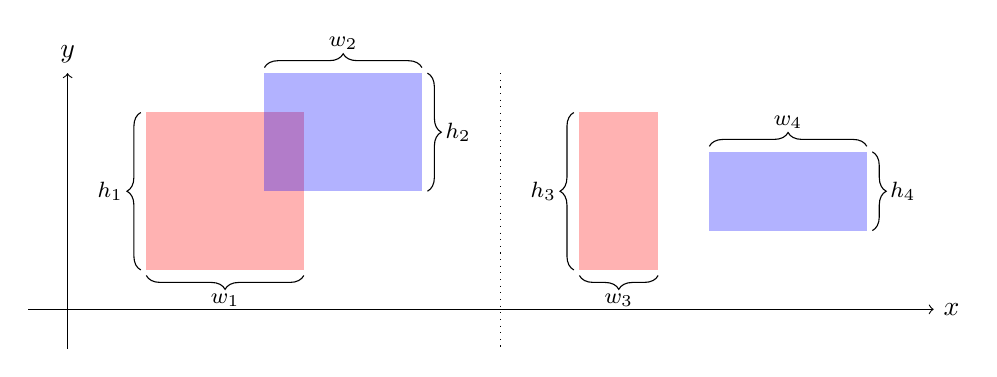
\begin{tikzpicture}[scale=1]

% Coordinates of Rectangle 1
\coordinate (A) at (1, .5);
\coordinate (B) at (3, .5);
\coordinate (C) at (3, 2.5);
\coordinate (D) at (1, 2.5);

% Coordinates of Rectangle 2
\coordinate (E) at (2.5, 1.5);
\coordinate (F) at (4.5, 1.5);
\coordinate (G) at (4.5, 3);
\coordinate (H) at (2.5, 3);

% Draw x/y axis
\draw[->] (-.5,0) -- (11,0) node[right] {\textbf{$x$}};
\draw[->] (0,-.5) -- (0,3) node[above] {\textbf{$y$}};
\draw[dotted] (5.5, 3) -- (5.5,-.5) node[above] {};

% Draw Rectangle 1 in transparent red
\fill[red, opacity=0.3] (A) -- (B) -- (C) -- (D) -- cycle;

% Draw Rectangle 2 in transparent blue
\fill[blue, opacity=0.3] (E) -- (F) -- (G) -- (H) -- cycle;

% Width labels for Rectangle 1
\draw[decorate, decoration={brace, amplitude=5pt, mirror, raise=2pt}] (A) -- (B) node[midway, below=5pt] {\footnotesize{}$w_1$};
\draw[decorate, decoration={brace, amplitude=5pt, raise=2pt}] (A) -- (D) node[midway, left=5pt] {\footnotesize{}$h_1$};

% Width labels for Rectangle 2
\draw[decorate, decoration={brace, amplitude=5pt, raise=2pt, mirror}] (G) -- (H) node[midway, above=5pt] {\footnotesize{}$w_2$};
\draw[decorate, decoration={brace, amplitude=5pt, raise=2pt, mirror}] (F) -- (G) node[midway, right=5pt] {\footnotesize{}$h_2$};

% Coordinates of Rectangle 3
\coordinate (I) at (6.5, .5);
\coordinate (J) at (7.5, .5);
\coordinate (K) at (7.5, 2.5);
\coordinate (L) at (6.5, 2.5);

% Coordinates of Rectangle 4
\coordinate (M) at (8.15, 1);
\coordinate (N) at (10.15, 1);
\coordinate (O) at (10.15, 2);
\coordinate (P) at (8.15, 2);

% Draw Rectangle 3 in transparent red
\fill[red, opacity=0.3] (I) -- (J) -- (K) -- (L) -- cycle;

% Draw Rectangle 4 in transparent blue
\fill[blue, opacity=0.3] (M) -- (N) -- (O) -- (P) -- cycle;

% Width labels for Rectangle 3
\draw[decorate, decoration={brace, amplitude=5pt, mirror, raise=2pt}] (I) -- (J) node[midway, below=5pt] {\footnotesize{}$w_3$};
\draw[decorate, decoration={brace, amplitude=5pt, raise=2pt}] (I) -- (L) node[midway, left=5pt] {\footnotesize{}$h_3$};

% Width labels for Rectangle 4
\draw[decorate, decoration={brace, amplitude=5pt, raise=2pt, mirror}] (O) -- (P) node[midway, above=5pt] {\footnotesize{}$w_4$};
\draw[decorate, decoration={brace, amplitude=5pt, raise=2pt, mirror}] (N) -- (O) node[midway, right=5pt] {\footnotesize{}$h_4$};
\end{tikzpicture}
\caption{Collision Detection Between Rectangles.}
\label{fig:collisiondetection}
\end{figure}

%\enlargethispage{1\baselineskip}
\begin{lstlisting}[language=MyJava]
abstract class GameObject {
  
  private int x;
  private int y;

  GameObject(int x, int y) {
    this.x = x;
    this.y = y;
  }
}
\end{lstlisting}


\begin{lstlisting}[language=MyJava]
abstract class AxisAlignedBoundingBoxObject extends GameObject {
  
  private int width;
  private int height;

  AxisAlignedBoundingBoxObject(int x, int y, int width, int height) {
    super(x, y);
    this.width = width;
    this.height = height;
  }

  /**
   * Determines whether this object collides with 
   * another AxisAlignedBoundingBoxObject.
   * @param obj instance of AxisAlignedBoundingBoxObject.
   * @return true if the objects overlap and false otherwise.
   */
  boolean collidesWith(AxisAlignedBoundingBoxObject obj) {
    return (this.getX() < obj.getX() + obj.width) &&
	   (this.getX() + this.width >= obj.getX()) &&
 	   (this.getY() < obj.getY() + obj.height)  &&
	   (this.getY() + this.height >= obj.height); 
  }
}
\end{lstlisting}

We declared an abstract class to extend another abstract class; which is perfectly acceptable. Because it makes no sense to instantiate an entity, in and of itself, called \ttt{AxisAlignedBoundingBoxObject}, we declare it as abstract, but we need it to contain the functionality of \ttt{GameObject}, which calls for the inheritance. Normally, we would immediately write an extensive test suite for \ttt{collidesWith}, but because we cannot instantiate an \ttt{AxisAlignedBoundingBox} directly, we cannot test \ttt{collidesWith} at the moment. In a couple of paragraphs, however, this will be possible, with the additions of \ttt{CircleObject} and \ttt{RectangleObject}.

%\enlargethispage{4\baselineskip}
\begin{lstlisting}[language=MyJava]
import static Assertions.assertAll;
import static Assertions.assertEquals;

class AxisAlignedBoundingBoxObjectTester {

  @Test
  void testCollidesWith() {
    AxisAlignedBoundingBoxObject o1 
      = new RectangleObject(30, 30, 1000, 2000);
    AxisAlignedBoundingBoxObject o2 
      = new RectangleObject(0, 0, 5, 5);
    AxisAlignedBoundingBoxObject o3 
      = new RectangleObject(400, 200, 750, 250);
    AxisAlignedBoundingBoxObject o4 
      = new RectangleObject(300, 100, 300, 200);
    AxisAlignedBoundingBoxObject o5 
      = new CircleObject(20, 30, 1000);
    AxisAlignedBoundingBoxObject o6 
      = new CircleObject(200, 250, 500);
    AxisAlignedBoundingBoxObject o7 
      = new CircleObject(30, 300, 1500);
    AxisAlignedBoundingBoxObject o8 
      = new CircleObject(90, 85, 200);
    assertAll(
      () -> assertTrue(o1.collidesWith(o2)),
      () -> assertTrue(o1.collidesWith(o4)),
      () -> assertTrue(o2.collidesWith(o3)),
      () -> assertTrue(o2.collidesWith(o8)),
      () -> assertTrue(o3.collidesWith(o5)),
      () -> assertTrue(o5.collidesWith(o4)),
      () -> assertTrue(o6.collidesWith(o7)),
      () -> assertTrue(o7.collidesWith(o3)));
  }
}
\end{lstlisting}

We need to translate our circles into axis-aligned bounding box, but what does that mean? In short, we convert the given radius into the corresponding diameter, and designate this diameter as the width and height of the bounding box. Rectangular objects, on other hand, need no such fancy translation, since a bounding box is a rectangle. Neither subclasses store their dimensions as instance variables, due to the fact that the superclass takes care of this for us.

The question that we anticipate many readers are thinking of is, why do we even distinguish objects of differing ``types'' if they both implement collision detection in the same fashion? Since we are working in the context of a game, the way we draw these objects is certainly different! Let's, for the sake of emphasizing the distinctions, design a \ttt{IDrawable} interface, which provides one method: \ttt{void draw(Graphics2D g2d)}, which gives us a \ttt{Graphics2D} object. We will not discuss, nor do we really care about the innards of a graphics library aside from the fact that it contains two primitive methods: \ttt{drawOval(int x, int y, int w, int h)} and \ttt{drawRect(int x, int y, int w, int h)}. Therefore our two object subclasses will implement \ttt{IDrawable} and override the method differently.

\enlargethispage{-4\baselineskip}
\begin{lstlisting}[language=MyJava]
interface IDrawable {
  
  /**
   * Provides a means of drawing primitive graphics.
   * The inner details of "Graphics2D" are not important to us; 
   * we care about the fact that we can use the following methods:
   * 
   * - drawOval(int x, int y, int w, int h);
   * - drawRect(int x, int y, int w, int h);
   */
  void draw(Graphics2D g2d); 
}
\end{lstlisting} 

%\enlargethispage{2\baselineskip}
\begin{lstlisting}[language=MyJava]
class CircleObject extends AxisAlignedBoundingBoxObject implements IDrawable {
  
  CircleObject(int x, int y, int r) { super(x, y, r * 2, r * 2); }

  @Override
  public void draw(Graphics2D g2d) {
    g2d.drawOval(this.getX(), this.getY(), 
                 this.getWidth(), this.getHeight());
  }
}
\end{lstlisting}

\begin{lstlisting}[language=MyJava]
class RectangleObject extends AxisAlignedBoundingBoxObject implements IDrawable {
  
  RectangleObject(int x, int y, int w, int h) { super(x, y, w, h); }
  
  @Override
  public void draw(Graphics2D g2d) {
    g2d.drawRect(this.getX(), this.getY(), 
                 this.getWidth(), this.getHeight());
  }
}
\end{lstlisting}

\myexample{A terminal argument parser is a program/function that interprets a series of arguments passed to another program and makes it easier for programmers to determine if a flag is enabled. Without one, many programmers often resort to using a complex series of conditional statements to check for the existence of a flag. Not only is this cumbersome, but it is prone to errors, and neither extendable nor flexible to different arrangements of arguments. In this example we will develop a small terminal argument parser.}

First, we need to design a class that represents an ``argument'' to a program. Arguments, as we described in Chapter~\ref{chapter-arrays-collections}, are space-separated string values that we pass to a program executable, which populate the \ttt{String[] args} array in the \ttt{main} method. In particular, however, we want to specify that an argument is not necessarily the values themselves, but are instead the flags, or instructions, passed to the executable. The simplest version of a flag is one that receives exactly one argument, which we will represent via an abstract \ttt{Argument} class. Later on, we want to be able to validate a flag with its given arguments, so the \ttt{Argument} class includes an abstract \ttt{boolean validate} method, that shall be overridden in all subclasses of \ttt{Argument}.

\begin{lstlisting}[language=MyJava]
import java.util.List;
import java.util.Map;

abstract class Argument {

  private String key;

  Argument(String key) { this.key = key; }

  String getKey() { return this.key; }

  abstract boolean validate(Map<String, List<String>> args);
}
\end{lstlisting}

From here, let's design two types of arguments: one that is optional and one that receives~$n$ arguments. Namely, an optional argument is one that is always valid, according to \ttt{validate}, because it does not necessarily need to exist. The~$n$-valued argument, on the other hand, requires that the associated passed flag contains exactly~$n$ values. For example, if we say that the \ttt{--input} flag requires exactly~$3$ arguments, then if we do not pass exactly three space-separated non-flag values, it fails to validate.

\begin{lstlisting}[language=MyJava]
import java.util.List;
import java.util.Map;

class OptionalArgument extends Argument {

  OptionalArgument(String key) { super(key); }

  @Override
  boolean validate(Map<String, List<String>> args) { return true; }
}
\end{lstlisting}

\begin{lstlisting}[language=MyJava]
import java.util.List;
import java.util.Map;

class NumberedArgument extends Argument {

  private final int NUM_REQUIRED_ARGS;

  NumberedArgument(String key, int n) {
    super(key);
    this.NUM_REQUIRED_ARGS = n;
  }

  @Override
  boolean validate(Map<String, List<String>> args) {
    if (!args.containsKey(this.getKey())) { return false; } 
    else { return args.get(this.getKey()).size() == this.NUM_REQUIRED_ARGS; }
  }
}
\end{lstlisting}

Now comes the argument parser itself, which receives a string array of argument values, much like \ttt{main}, and extracts out the flags and arguments into a \ttt{Map<String, List<String>{}>} where the key represents the flag and the value is a list of the arguments to said flag. We also store a \ttt{Set<Argument>} to allow the programmer to designate arguments to the parser. The idea is straightforward: while traversing over \ttt{args}, if we encounter a string that begins with a double dash `\ttt{--}', it is qualified as a flag and the following arguments, up to another flag, are marked as arguments to the flag. We add these to the respective map as described before, and continue until we run out of elements in the array.

\begin{lstlisting}[language=MyJava]
import java.util.HashMap;
import java.util.HashSet;
import java.util.Map;
import java.util.Set;

class ArgumentParser {

  private final Map<String, List<String>> PARSED_ARGS;
  private final Set<Argument> ARGS;

  ArgumentParser(String[] args) {
    this.ARGS = new HashSet<>();
    this.PARSED_ARGS = new HashMap<>();
    String currKey = null;
    for (String arg : this.ARGS) {
      if (arg.startsWith("--")) {
        currKey = arg.split("--")[1];
        this.PARSED_ARGS.putIfAbsent(currKey, new ArrayList<>());
      } else if (currKey != null) {
        this.PARSED_ARGS.get(currKey).add(arg);
      }
    }
  }

  void addArgument(Argument arg) { this.ARGS.add(arg); }

  List<String> getArguments(String key) {
    return this.PARSED_ARGS.containsKey(key) ? this.PARSED_ARGS.get(key) : null;
  }
}
\end{lstlisting}

The \ttt{parseArguments} method returns whether or not the supplied arguments are valid according to the arguments populated via \ttt{addArgument}. Using streams, we verify that, after invoking \ttt{validate} on every argument, each separate call returns true, meaning that all arguments are valid and correct. Because it might be useful to return the associated arguments to a flag from a programmer's perspective who uses this parser, we include a \ttt{getArguments} method to return the list of arguments passed to a flag.

\begin{lstlisting}[language=MyJava]
import java.util.HashMap;
import java.util.HashSet;
import java.util.Map;
import java.util.Set;

class ArgumentParser {

  /**
   * Determines whether or not all of the arguments in the stored field are "valid."
   * @return true if all arguments are valid, false otherwise.
   */
  boolean parseArguments() {
    return this.arguments.stream()
                         .allMatch(e -> e.validate(this.parsedArguments));
  }
}
\end{lstlisting}

\subsubsection*{The ASPL Interpreter}
\myexample{Inheritance is a truly powerful programming language construct, and we will now attempt to describe its beauty through the design of a mini-project. Said mini-project will encompass writing a small programming language called ASPL, or ``A Simple Programming Language.''\footnote{Originally, we called the interpreter APL, or ``A Programming Language.'' We changed its name to include the extra `S' so as to not cause confusion between our implementation and the actual language called APL~\Citep{apl}. If you want to have some ``fun,'' take a slight detour and go explore \emph{that} language!} Programming language syntax and semantics, collectively, require a lot of knowledge outside the domain and scope of this text, but we will see that, even with our somewhat limited arsenal of tools, we can construct a fairly powerful programming language. Our language will start off as a recreation of the interpreter from our section on interfaces, but contains modifications to make it more flexible.}

As a means of motivation, let's write a few programs in this language to show its capabilities. The first listing is a simple program to add two numbers together. The second listing binds two variables, and if their sum is equal to 42, then the result is 100, otherwise it is zero. The third listing declares a variable, followed by a conditional, both cases of which contain another binding of a variable, closing off with a product operation.

\noindent % Prevents indentation at the beginning of the line
\begin{minipage}[t]{0.32\textwidth}
\begin{lstlisting}[language=MyScheme, frame=single]
(+ 25 17)
(*;\phantom{.};*)
(*;\phantom{.};*)
(*;\phantom{.};*)
(*;\phantom{.};*)
(*;\phantom{.};*)
(*;\phantom{.};*)
(*;\phantom{.};*)
\end{lstlisting}
\end{minipage}%
\hfill % Fills the horizontal space between the minipages
\begin{minipage}[t]{0.32\textwidth}
\begin{lstlisting}[language=MyScheme, frame=single]
(let ([x 10])
  (let ([y 32])
    (if (eq? (+ x y) 42)
        100
        0)))

(*;\phantom{.};*)
(*;\phantom{.};*)
\end{lstlisting}
\end{minipage}%
\hfill % Fills the horizontal space between the minipages
\begin{minipage}[t]{0.32\textwidth}
\begin{lstlisting}[language=MyScheme, frame=single]
(let ([z 95])
  (if (eq? (- 100 5) z)
      (let ([w -10])
        (* w z 2))
      (let ([w -5])
        (* z w -2))))
(*;\phantom{.};*)
(*;\phantom{.};*)
\end{lstlisting}
\end{minipage}

Programming language syntax is often broken up into the nodes of an \emph{abstract syntax tree}, which at a quick glance is nothing more than a description of the operations of a language. To begin, we need to describe our programming language capabilities. 
To keep things simple, our language will contain integers, variables, a few arithmetic operators, and conditionals. 
It's important to note that, because we are glossing over the innards of lexing and  parsing, all of our tests will exist in the form of abstract syntax trees.
We want an abstract AST node class from which every other AST node inherits. Then, we can design purpose-specific nodes that do what we wish. 
Every abstract syntax tree has a list of children node. We will also define a \texttt{toString} method that will print out the abstract syntax tree in a readable format. 
Our abstract syntax tree class uses two constructors: one that receives a list of abstract syntax tree nodes, and another that is variadic over the \ttt{AstNode} type. We implement two different constructors for convenience purposes during testing.

Each abstract syntax tree should be evaluable as a means of reducing the expression to its simplest form. For example, numbers and booleans, the literals of our language, resolve to themselves. Primitive operations apply the operation to its arguments, then ultimately reduce to a value. Conditionals resolve to either of its branches, and ``let'' bindings resolve to its body. We will cover each case one-by-one as we cover the material. For now, though, the abstract syntax tree node class contains the \ttt{eval} method, which denotes how a node is to be evaluated.

\newpage
\begin{lstlisting}[language=MyJava]
import java.util.List;

abstract class AstNode {

  private final List<AstNode> CHILDREN;  
 
  AstNode(List<AstNode> children) { 
    this.CHILDREN = children; 
  }

  AstNode(AstNode... children) { 
    this(List.of(children)); 
  }

  abstract AstNode eval();

  List<AstNode> getChildren() { 
    return this.CHILDREN; 
  }

  public abstract String toString();
}
\end{lstlisting}

From here, the simplest two abstract syntax tree nodes are \ttt{NumNode} and \ttt{BoolNode}, corresponding to numbers and booleans literals respectively.
Nodes that encapsulate sole values, e.g., numbers and booleans, are examples of literals, and all literals are evaluated/treated the same way.
As such, let's design the generic and abstract \ttt{LiteralNode<T>} class, which all literal types extend, those for our purposes being \ttt{NumNode} and \ttt{BoolNode}.\footnote{We say, ``for our purposes,'' because the language could also support string or character literals.}

A \ttt{LiteralNode<T>} stores an immutable object of type \ttt{T}.
Literal values resolve to themselves and only themselves, which means that they return \ttt{this} as the object in \ttt{LiteralNode}'s \ttt{eval} method.
The \ttt{LiteralNode} class overrides \ttt{equals}, \ttt{hashCode}, and \ttt{toString} to compare literals, return the hash code of the stored instance variable, and ``stringify'' the instance variable respectively.
Designing the \ttt{LiteralNode} class in this fashion makes designing the subclasses easier and significantly less redundant, because \ttt{NumNode} and \ttt{BoolNode} need to only provide constructors that invoke the superclass.

\begin{lstlisting}[language=MyJava]
import static Assertions.assertAll;
import static Assertions.assertEquals;

class AstTest {

  @Test
  void testNumNode() {
    assertEquals("42", new NumNode("42").toString());
  }

  @Test
  void testBoolNode() {
    assertEquals("true", new BoolNode("true").toString());
    assertEquals("false", new BoolNode("false").toString());
  }  
}
\end{lstlisting}

\newpage
\begin{lstlisting}[language=MyJava]
import java.util.Objects;

abstract class LiteralNode<T> extends AstNode {

  private final T VALUE;

  LiteralNode(T value) { this.VALUE = value; }

  @Override
  AstNode eval(Environment env) { return this; }

  @Override
  public boolean equals(Object o) {
    if (!(o instanceof LiteralNode)) { return false; } 
    else { return this.VALUE.equals(((LiteralNode<?>) o).VALUE); }
  }

  @Override
  public int hashCode() { return Objects.hashCode(this.VALUE); }

  @Override
  public String toString() { return this.VALUE.toString(); }

  T getValue() { return this.VALUE; }
}
\end{lstlisting}

\begin{lstlisting}[language=MyJava]
final class NumNode extends LiteralNode<Double> {

  NumNode(double value) { super(value); }

  NumNode(String value) { super(Double.parseDouble(value)); }
}
\end{lstlisting}

% \newpage
\begin{lstlisting}[language=MyJava]
final class BoolNode extends LiteralNode<Boolean> {

  BoolNode(boolean value) { super(value); }

  BoolNode(String value) { this(Boolean.parseBoolean(value)); }
}
\end{lstlisting}

The next logical step is to add primitive operations via \ttt{PrimNode}. 
A primitive operator is an operation akin to addition, subtraction, value equality, and so forth. 
Primitive operators receive any number of arguments, and the behavior of which is handled as a case analysis of the \ttt{eval} method. 

Though, evaluating a primitive operation is not as simple as applying the operator to its arguments. 
Consider the following code segment, where we have the primitive operation \ttt{+} applied to two more primitive operations `\ttt{*}' and `\ttt{-}.' 
We see that it is impossible to directly apply the plus operation to the two primitives, because addition only works over \ttt{NumNode} values and not \ttt{AstNode} instances. 
So, when applying a primitive operation, we must first recursively evaluate its children nodes, i.e., the arguments. 
The list of arguments is converted into a stream, where we map the \ttt{eval} method over each element. 
Afterwards, we write the aforementioned case analysis on the operation. 
For the addition operator, we sum all the values of the children nodes. 
Even though each node is definitionally an \ttt{AstNode}, we can safely cast them to \ttt{NumNode} because we know that the operation is semantically valid only over numbers (the same logic applies to other such primitive operators).

\enlargethispage{-1\baselineskip}
\begin{lstlisting}[language=MyJava]
import static Assertions.assertAll;
import static Assertions.assertEquals;

class AstTest {

  @Test
  void testPrimNode() {
    assertAll(
      () -> assertEquals(new NumNode(42),
                          new PrimNode("+", 
                           new NumNode(25), 
                           new NumNode(17)).eval());
      () -> assertEquals(new NumNode(42),
                          new PrimNode("-", 
                           new NumNode(97), 
                           new NumNode(55)).eval());                         
      () -> assertEquals(new NumNode(42),
                          new PrimNode("*", 
                           new NumNode(6), 
                           new NumNode(1), 
                           new NumNode(7)).eval());
      () -> assertEquals(new BoolNode(true),
                          new PrimNode("eq?",
                           new PrimNode("+", 
                            new NumNode(5),
                            new NumNode(37)),
                            new NumNode(42)).eval())):
      () -> assertEquals(new NumNode(42),
                          new PrimNode("+",
                           new PrimNode("*",
                            new NumNode(2), 
                             new PrimNode("-",
                              new NumNode(57),
                              new NumNode(23))),
                            new PrimNode("-",
                             new NumNode(4),
                             new NumNode(30))));           
  }
}
\end{lstlisting}

% \newpage %ugh
% \enlargethispage{1\baselineskip}
\begin{lstlisting}[language=MyJava]
import java.util.List;

final class PrimNode extends AstNode {

  private final String OP;

  PrimNode(String op, AstNode... children) {
    super(children);
    this.OP = op;
  }

  @Override
  public String toString() {
    return String.format("(%s %s)",this.OP, this.getChildren().toString());
  }

  /**
   * Interpret a primitive operation.
   * @param env the environment in which to interpret the operation.
   * @return The result of the primitive operation.
   */
  @Override
  AstNode eval(Environment env) {
    List<AstNode> operands = this.getChildren().stream()
                                               .map(n -> n.eval(env))
                                               .toList();
    switch (this.OP) {
      case "+": return this.primPlus(operands, env);
      case "-": return this.primMinus(operands, env);
      case "*": return this.primProduct(operands, env);
      case "eq?": return this.primEq(operands, env);
      default: return null;
    }
  }

  private AstNode primPlus(List<AstNode> args, Environment env) {
    return new NumNode(args.stream()
                           .map(t -> ((NumNode) t).getValue())
                           .sum());
  }

  private AstNode primMinus(List<AstNode> args, Environment env) {
    double res = ((NumNode) args.get(0)).getValue();
    for (int i = 1; i < args.size(); i++) {
      res -= ((NumNode) args.get(i)).getValue();
    }
    return new NumNode(res);
  }

  private AstNode primProduct(List<AstNode> args, Environment env) {
    return new NumNode(args.stream()
                           .map(t -> ((NumNode) t).getValue())
                           .reduce(1.0, (a, c) -> c * a));
  }

  private AstNode primEq(List<AstNode> args, Environment env) {
    return new BoolNode(args.get(0).equals(args.get(1)));
  }
}
\end{lstlisting}

Adding the equality comparison operator provides a pathway to designing the conditional expression, namely \ttt{IfNode}. 
An \ttt{IfNode} contains three children nodes: a predicate, a consequent, and an alternative. 
The \ttt{eval} method of an \ttt{IfNode} evaluates the predicate, and if it is true, evaluates the consequent, otherwise it evaluates the alternative. 
The predicate \emph{must} resolve to a boolean, assuming the program is well-formed. 
Because we only care about well-formed programs, we do not need to check if the predicate is a boolean, and can safely cast it to a \ttt{BoolNode} when evaluating the respective abstract syntax tree node.

\newpage
\begin{lstlisting}[language=MyJava]
import static Assertions.assertAll;
import static Assertions.assertEquals;

class AstTest {
  
  @Test
  void testIfNode() {
    assertAll(
      () -> assertEquals(new NumNode(100),
                          new IfNode(new BoolNode(true),
                                     new NumNode(100),
                                     new NumNode(0)).eval()),
      () -> assertEquals(new BoolNode(false),
                          new IfNode(new PrimNode("eq?", 
                                       new NumNode(5), 
                                       new NumNode(5)),
                                     new BoolNode(true),
                                     new BoolNode(false)).eval()));
  }
}  
\end{lstlisting}

With numbers, booleans, primitive operations, and conditionals taken care of, we now come to the challenging part: variable bindings. 
We need a way of introducing variable bindings to their values, so we shall take a hint from functional programming languages via the \ttt{LetNode} class. 
The \ttt{LetNode} class has three children: a variable name, a value, and a body. 
The variable name is a string, with the value and body both being abstract syntax tree nodes. 
The \ttt{LetNode} class will have a \ttt{toString} method that will return a string in the form of \ttt{(let ([<var> <exp>]) <body>)}. 
In tandem, we will also write the \ttt{VarNode} class, which represents variable placeholders. In order to do anything meaningful with both classes, we need to discuss the scope of a variable and how to handle the encompassing issues.

The \emph{scope of a variable} refers to its lifetime.
Consider the following program in our language. Initially, the program has no variable bindings. 
After encountering the \ttt{let}, we enter a scope that binds the variable identifier~$x$ to~$5$. 
The body of this \ttt{let} is, therefore, the \emph{scope} of~$x$. 
Inside this body, we encounter yet another variable, namely~$y$, which binds~$y$ to~$10$. 
The body of this \ttt{let} is the scope of~$y$. Outside the scope of the body,~$y$ is non-existent.
\begin{verbnobox}[\small]
(let ([x 5])
  (let ([y 10])
    (* x y)))
\end{verbnobox}
When executing this program in our heads, we know intuitively that~$x$ refers to~$5$ and~$y$ refers to~$10$. 
To write a programming language, though, we need to formalize the notion of ``variable lookup.'' That is, we must define how to associate variable identifiers to values. 
Of course, the best data structure for value association is a map, and indeed, this is the structure we will use.

Programming languages use \emph{environments} to associate identifiers to values. 
Upon encountering a variable declaration, we extend the current environment to contain the new binding. 
This begs the question, ``Why not just modify the environment?'' 
The answer is that we want to respect the scope of variables. 
Modifying the environment changes the environment for all scopes, an undesired trait. 
In other words, if we mutate a variable binding in the existing environment, the variable's lifetime is extended to the entire program rather than to the scope in which it was declared.
Instead, we \emph{extend} the environment, which establishes a link between the current environment and the newly-declared environment. 
This way, we can look up variables in the current environment, and if they do not exist, we can look them up in the parent environment. 
If the variable does not exist in the parent environment, we return a \ttt{null} value.

Environments, accordingly, contain two instance variables: a \ttt{Map<String, AstNode} and a \ttt{Environment} parent pointer. Our environment class comprises two methods: \ttt{lookup} and \ttt{extend}. 

The \ttt{lookup} method attempts to find a binding for the given variable identifier using the aforementioned approach. The \ttt{extend} method instantiates a new environment, whose parent is the current existing environment. This newly-instantiated environment, importantly, contains a new variable binding. Remember that the environment is a functional data structure, meaning that it is immutable.

% \enlargethispage{-8\baselineskip}
\begin{lstlisting}[language=MyJava]
import static Assertions.assertAll;
import static Assertions.assertEquals;

class EnvironmentTester {
  
  @Test
  void testEnvironment() {
    Environment root = new Environment();
    Environment e1 = root.extend("x", new NumNode(5));
    Environment e2 = e1.extend("y", new NumNode(6));
    assertAll(
      () -> assertEquals(new NumNode(5), e2.lookup("x")),
      () -> assertEquals(new NumNode(6), e2.lookup("y")),
      () -> assertEquals(null, e2.lookup("z")));
  }
}
\end{lstlisting}

% \enlargethispage{3\baselineskip}
\begin{lstlisting}[language=MyJava]
import java.util.HashMap;
import java.util.Map;

final class Environment {

  private final Map<String, AstNode> ENV;
  private final Environment PARENT;

  Environment(Environment parent) { 
    this.ENV = new HashMap<>(); 
    this.PARENT = parent; 
  }

  Environment() { this(null); }

  AstNode lookup(String id) {
    if (this.ENV.containsKey(id)) { return this.ENV.get(id); }
    else if (this.PARENT != null) { return this.PARENT.lookup(id); }
    else { return null; }
  }

  Environment extend(String id, AstNode value) {
    Environment env = new Environment(this);
    env.ENV.put(id, value);
    return env;
  }
}
\end{lstlisting}

Now we can design the \ttt{VarNode} class. 
The apparent question is, ``How do we evaluate a variable?'' 
Using environments, we look up the variable identifier and return its associated abstract syntax tree. 
But, where does the environment come from? 
Environments are passed as an argument to the \ttt{eval} method, which means that all previously-existing \ttt{eval} methods must be updated to accept an environment as an argument.

Variable nodes, on their own, are simple yet relatively useless, and simply cannot exist without a means of introducing them into the environment context. 
This is where the \ttt{LetNode} class comes into play. 
The \ttt{LetNode} class introduces a new variable binding into the environment. 
A \ttt{LetNode} has two abstract syntax tree children: an expression and a body. The expression is evaluated and its value is bound to the provided variable identifier in an \emph{extended environment} $e_2$, whose parent is the current environment~$e_1$. The body of the \ttt{LetNode} is evaluated with respect to the extended environment, i.e.,~$e_2$.

\begin{lstlisting}[language=MyJava]
import static Assertions.assertAll;
import static Assertions.assertEquals;

class AstTest {

  @Test
  void testLetNode() {
    Environment env = new Environment();
    assertAll(
      () -> assertEquals(new NumNode(42),
                         new LetNode("x", 
                          new NumNode(42),
                          new VarNode("x")).eval(env)),
      () -> assertEquals(new NumNode(42),
                         new LetNode("x", 
                          new NumNode(1),
                          new LetNode("y", 
                           new NumNode(41),
                           new PrimNode("+", 
                            new VarNode("x"), 
                            new VarNode("y")))).eval(env)));
  }
}
\end{lstlisting}

\enlargethispage{-2\baselineskip}
\begin{lstlisting}[language=MyJava]
final class VarNode extends AstNode {

  private final String NAME;

  VarNode(String name) {
    super();
    this.NAME = name;
  }

  @Override
  public String toString() { 
    return this.NAME; 
  }

  /**
   * Interpret a variable. We look up the variable in the environment and
   * return the value associated with it.
   * @param env the environment in which to interpret the variable.
   * @return The result of the variable lookup after interpretation.
   */
  @Override
  AstNode eval(Environment env) {
    String id = this.NAME;
    AstNode res = env.lookup(id);
    return res.eval(env);
  }

  String getName() {
    return this.NAME;
  }
}
\end{lstlisting}
  
\begin{lstlisting}[language=MyJava]
final class LetNode extends AstNode {

  private final String ID;

  LetNode(String id, AstNode exp, AstNode body) {
    super(exp, body);
    this.ID = id;
  }
  
  @Override
  public String toString() {
    AstNode e = this.getChildren().get(0);
    AstNode b = this.getChildren().get(1);
    return String.format("(let ([%s %s]) %s)", this.ID, e, b);
  }

  /**
   * Interprets a let statement. The body is evaluated in the extended env.
   * The extended environment contains the binding introduced by the ID.
   * The identifier's binding expression "exp" is evaluated in "env".
   * @param env The environment to use for the let.
   * @return The result of the let statement.
   */
  @Override
  AstNode eval(Environment env) {
    String id = this.ID;
    AstNode exp = this.getChildren().get(0);
    AstNode body = this.getChildren().get(1);

    // Interpret the expression and convert it into its AST.
    AstNode newExp = exp.eval(env);
    Environment e1 = env.extend(id, newExp);
    return body.eval(e1);
  }
}
\end{lstlisting}

Finally, at long last, we can write some comprehensive tests! 
We will store each test in the \ttt{InterpTester} class, which polymorphically executes \ttt{eval} on the abstract syntax tree instances. 
All examples are initialized with an empty environment, because there are no (locally-declared) variable bindings at the start of a program. 
Unfortunately, we still have to write the programs as a series of compositional abstract syntax trees, but the problems of lexing and parsing raw string input into an abstract syntax tree are reserved for another time (or perhaps a separate course altogether). 

\enlargethispage{-2\baselineskip}
\begin{lstlisting}[language=MyJava]
import static Assertions.assertAll;
import static Assertions.assertEquals;
  
class InterpTester {
  
  @Test
  void testEval() {
    assertAll(
      () -> assertEquals(new NumNode("42"),
                         new NumNode("42").eval(new Environment())),
      () -> assertEquals(new BoolNode(true),
                         new PrimNode("eq?",
                          new NumNode(42),
                          new PrimNode("-",
                           new NumNode(100),
                           new NumNode(58))).eval(new Environment())),
      () -> assertEquals(new NumNode("42"),
                         new LetNode("x", 
                          new NumNode("42"), 
                          new VarNode("x")).eval(new Environment())),
      () -> assertEquals(new NumNode("42"),
                         new LetNode("x", new NumNode("1"),
                          new LetNode("y", new NumNode("41"),
                           new PrimNode("+", 
                            new VarNode("x"), 
                            new VarNode("y")))).eval(new Environment())));
  }
}
\end{lstlisting}

Object-oriented programs with inheritance should be structured as a sequence of specific subclasses that extend an abstract class, as we have demonstrated with the different abstract syntax tree node types, and the root \ttt{AstNode} abstract class. 


\newpage
\section{Exercises}

\myexercise{1}{chapter-classes}{Design the \ttt{Car} class, which stores a \ttt{String} representing the car's make, a \ttt{String} representing the car's model, and an \ttt{int} representing the car's year. Its constructor should receive these three values and store them in the instance variables. Be sure to write instance accessor and mutator methods for modifying all three fields. That is, you should write \ttt{getMake()}, \ttt{setMake(String s)}, and so forth, to access and modify the fields directly.}

\myexercise{1}{chapter-classes}{Design the \ttt{Dog} class, which stores a \ttt{String} representing the breed, a \ttt{String} representing its name, and an \ttt{int} representing its age in years. You should also store a boolean to keep track of whether or not the dog is a puppy. A dog is a puppy if it is less than two years old. Its constructor should receive these three values and store them in the instance variables. Be sure to write instance accessor and mutator methods for modifying all three fields. That is, you should write \ttt{getBreed()}, \ttt{setBreed(String s)}, and so forth, to access and modify the fields directly.}

\myexercise{1}{chapter-classes}{Design the \ttt{Person} class, which stores a \ttt{String} representing the person's first name, a \ttt{String} representing the person's last name, and an \ttt{int} representing the person's age in years. Its constructor should receive these three values and store them in the instance variables. Be sure to write instance accessor and mutator methods for modifying all three fields. That is, you should write \ttt{getFirstName()}, \ttt{setFirstName(String s)}, and so forth, to access and modify the fields directly.}

% \myexercise{1}{chapter-classes}{Design the \ttt{Employee} class, which stores the employee's first and last names as strings, their birth year as an integer, their yearly salary as a double (we will assume that all employees are paid some value greater than zero), and their employee ID as a string.}
    
% To make things interesting, assume that an employee's ID is not alterable and must be set in the constructor. The employee ID is constructed using the first five characters of their last name, the first letter of their first name, and the last two digits of their birth year. For instance, if the employee's name is \ttt{Joshua Crotts} and their birth year is \ttt{1999}, their employee ID is \ttt{CrottJ99}. Its constructor should receive the name, birth year, and salary as parameters, but build the employee ID from the name and birth year.

% The instance variables, accessors, and mutators (where applicable) should be named as follows:
% \begin{itemize}
%     \item \ttt{id}, \ttt{getId}.
%     \item \ttt{firstName}, \ttt{getFirstName}.
%     \item \ttt{lastName}, \ttt{getLastName}.
%     \item \ttt{birthYear}, \ttt{getBirthYear}.
%     \item \ttt{salary}, \ttt{getSalary}, \ttt{setSalary}
% \end{itemize}

% Then, design the following methods:

% \begin{enumerate}[label=(\alph*)]
%   \item \ttt{void bonus()} method, which updates the salary of an employee. Calling \ttt{bonus} on an employee increases their salary by ten percent.
%   \item Override the \ttt{public boolean equals(Object o)} and \ttt{public String toString()} methods from the \ttt{Object} class to compare two employees by their employee ID and to print the employee's name, birth year, salary, and employee ID respectively separated by commas and a space. Do not add a comma and space after the last field.
% \end{enumerate}

\myexercise{2}{chapter-classes}{In this exercise you will design a class for storing employees. This relies on having the \ttt{Employee} class and its subclasses from the chapter available.}
\begin{enumerate}[label=(\alph*)]
    \item Design the \ttt{Job} class, which stores a list of employees \ttt{List<Employee>} as an instance variable. Whether you choose to instantiate it as an \ttt{ArrayList} or a \ttt{LinkedList} is up to you and makes little difference for this particular question. Its constructor should receive no arguments. The instance variable, along with its accessor and mutator, should be named \ttt{employees}, \ttt{getEmployees}, and \ttt{setEmployees} respectively.
    \item Design the \ttt{void addEmployee(Employee e)} method, which adds an employee to the \ttt{Job}.
    \item Design the \ttt{void removeEmployee(Employee e)} method, which removes an employee from the \ttt{Job}.
    \item Design the \ttt{Optional<Double> computeAverageSalary()} method, which returns the average salary of all employees in the \ttt{Job}. If there are no employees, return an empty \ttt{Optional}.
    \item Design the \ttt{Optional<Employee> highestPaid()} method, which returns the employee whose salary is the highest of all employees in the \ttt{Job}. If there are no employees, return an empty \ttt{Optional}.
    \item Override the \ttt{public String toString()} method to print out the list of employees in the \ttt{Job}. To make this easy, you can simply invoke the \ttt{toString} method from the \ttt{List} implementation.
\end{enumerate}

\newpage %ugh
\myexercise{2}{chapter-classes}{In this exercise you will design a simple music system, similar to Spotify.}
\begin{enumerate}[label=(\alph*)]
  \item Design the \ttt{Song} class, which stores its \ttt{title}, \ttt{artist}, \ttt{genre}, and \ttt{length}. The first three fields are strings and the last is an integer. Create the accessor methods, then override \ttt{equals}, \ttt{hashCode}, and \ttt{toString}. You may choose how to override \ttt{toString}.
  \item Design the \ttt{Playlist} class, which stores the title of the playlist and a set of the songs in the list. In this class, create the accessor methods, then override \ttt{equals}, \ttt{hashCode}, and \ttt{toString}. Finally, design the \ttt{boolean addSong(Song s)} that attempts to add~$s$ to the set of songs. If it already exists, return false. Otherwise, add the song to the set and return true.
  \item Design the \ttt{User} class, which stores their name and a list of playlists. Its constructor should receive the name and assign it to the respective instance variable. Instantiate the list to a new \ttt{ArrayList}. Create the accessor methods, then override \ttt{equals}, \ttt{hashCode}, and \ttt{toString}.
  \begin{enumerate}[label=(\roman*)]
    \item Design the \ttt{boolean createPlaylist(String t, Song... S)} method, which receives a playlist title~$t$ and a variadic number of songs~$S$, attempts to create a playlist with the title$~t$. If it already exists, return false and do nothing else. Otherwise, declare a new \ttt{Playlist} to their list and add to it the given songs.
  \end{enumerate}
  \item Design the \ttt{MusicSystem} class, which stores a list of users and a set of all the songs in the system. In the constructor, instantiate these to an \ttt{ArrayList} and \ttt{HashSet} respectively.
  \begin{enumerate}[label=(\roman*)]
    \item Design the \ttt{void addUser(User u)} method that receives a user~$u$ and adds them to the list of users.
    \item Design the \ttt{boolean addSong(User u, String t, Song s)} method that, when given a user~$u$, a playlist title~$t$, and a song~$s$, adds $s$ to $u$'s playlist with the title~$t$. If~$u$ does not exist or~$t$ is not a title in a playlist authored by~$u$, return false.
    \item Design the \ttt{Map<User, Song> getLongestSong()} method that returns the longest (length) song out of all the songs that a user has in their playlists. If the user has no playlists nor any songs in the playlists, do not add that user to the map.
  \end{enumerate}
\end{enumerate}

\myexercise{2}{chapter-classes}{In this exercise you will create two classes: \ttt{Chocolate} and \ttt{ChocolateBox} to store a two-dimensional array of chocolate pieces.}
\begin{enumerate}[label=(\arabic*)]
  \item Design the \ttt{Chocolate} class, which stores a string denoting its kind, and an integer representing its weight in ounces.

  \item Design the \ttt{ChocolateBox} class, which stores a \ttt{Chocolate[][]} array as an instance variable. Its constructor should receive the number of rows and columns of the box. 
  \begin{enumerate}[label=(\roman*)]
    \item Design the \ttt{int numberOfChocolates()} method that returns the number of non-\ttt{null} instances of \ttt{Chocolate} that are in the \ttt{ChocolateBox}.
    \item Design the \ttt{void shuffleChocolate()} method, which randomizes the elements in the box. 
    How you shuffle them is up to you, as long as it is a sufficient shuffle (and not just, for example, a linear shift of all chocolates).
    \item Design the \ttt{int removeFirst(String kind)} method, which removes the first occurrence, from the top, of the~\ttt{kind} of chocolate. Return what position was removed, assuming positions are numbered from~$1$ to~$n$, ordered from left to right, then top to bottom (similar to a standard calendar). If there are no~\ttt{kind} of chocolates in the box, return~\ttt{-1}.
    \item Design the \ttt{ChocolateBox allergyBox(String kind)} method, which returns a new \ttt{ChocolateBox} where all \ttt{kind} of chocolates are removed. If there are \ttt{null} spots in between the chocolates of the old box, shift the chocolates over accordingly. Consider the following \ttt{ChocolateBox}:
    % \newcolumntype{C}[1]{>{\centering\arraybackslash}m{#1}}
    \newcolumntype{C}[1]{>{\centering\arraybackslash}p{#1}} % Centered columns with fixed width

    % Table with 2x2 square cells, each 1cm x 1cm
    \renewcommand{\arraystretch}{2.5} % Adjust the row height to make cells square
    \begin{figure}[H]
      \centering
      \begin{tabular}{|C{1cm}|C{1cm}|C{1cm}|C{1cm}|C{1cm}|}
      \hline
      \emph{Dark} & \emph{White} & \emph{Milk} & \emph{Nut} & \emph{Sweet}\\ \hline
      \ttt{null} & \emph{Nut} & \emph{Dark} & \ttt{null} & \ttt{null}\\ \hline
      \emph{White} & \emph{Sweet} & \emph{Nut} & \ttt{null} & \emph{Nut}\\ \hline
      \end{tabular}
    \end{figure}
  \end{enumerate}

  Invoking \ttt{allergyBox("Nut")} on this box would return the following \ttt{ChocolateBox}:

  \newcolumntype{C}[1]{>{\centering\arraybackslash}p{#1}} % Centered columns with fixed width

    % Table with 2x2 square cells, each 1cm x 1cm
  \renewcommand{\arraystretch}{2.5} % Adjust the row height to make cells square
  \begin{figure}[H]
    \centering
    \begin{tabular}{|C{1cm}|C{1cm}|C{1cm}|C{1cm}|C{1cm}|}
    \hline
    \emph{Dark} & \emph{White} & \emph{Milk} & \emph{Sweet} & \emph{Dark}\\ \hline
    \emph{White} & \emph{Sweet} & \ttt{null} & \ttt{null} & \ttt{null}\\ \hline
    \ttt{null} & \ttt{null} & \ttt{null} & \ttt{null} & \ttt{null}\\ \hline
    \end{tabular}
  \end{figure}
\end{enumerate}

\myexercise{2}{chapter-classes}{In this exercise you will design a \emph{linear congruential generator}: a pseudorandom number generation algorithm. In particular, the C programming language standard library defines two functions: \ttt{rand} and \ttt{srand}. The latter sets the \emph{seed} for the generator, and \ttt{rand} returns a random integer between $[0, 2^{15})$. The formula for this generator is a recurrence relation:}
\begin{align*}
    \emph{next} &= |r_n \cdot 1103515245 + 12345|\\
    r_{n+1} &= \left(\dfrac{\emph{next}}{2^{16}}\right)\;\%\;2^{15};
\end{align*}

\begin{enumerate}[label=(\alph*)]
    \item Design the \ttt{LcgRandom} class, which implements this behavior. In particular, it should have two constructors: one that receives a seed value $s$, and another that sets the seed to one. The seed initializes the value of $r_0$.
    \item Design the \ttt{int genInt()} method, which returns a random integer between $0$ and $2^{15}$ using this algorithm.
    \item Design the \ttt{IntStream stream()} method, which returns a stream of random numbers that uses \ttt{genInt} to generate numbers. Hint: use \ttt{generate}!
    \item Design the \ttt{genInt(int b)} method that returns an integer between $[0, b]$. Note that $0 \leq b < 2^{15}$; you do not need to account for values outside of this range. Do \textbf{not} simply loop until you find a value between that range; instead, use modulus to your advantage.
\end{enumerate}

\newpage %ugh
\myexercise{3}{chapter-classes}{This question has six parts.}

\begin{enumerate}[label=(\alph*)]
    \item Design the \ttt{Matrix} class, which stores a two-dimensional array of integers. Its constructor should receive two integers~$m$~and~$n$ representing the number of rows and columns respectively, as well as a two-dimensional array of integers (you may assume that the number of rows and columns of the passed array are equal to~$m$ and~$n$). Copy the integers from the passed array into an instance variable array. Do \emph{not} simply assign the provided array to the instance variable!
    \item Design the \ttt{void set(int i, int j, int val)} method, which sets the value at row~$i$ and column~$j$ to \ttt{val}. If the row or column is out of bounds, do nothing.
    \item Design the \ttt{boolean add(Matrix m)} method, which adds the values of the passed matrix to the current matrix. If the dimensions of the passed matrix do not match the dimensions of the current matrix, return false and do not add the matrix.
    \item Design the \ttt{boolean multiply(Matrix m)} method, which multiplies the values of the passed matrix to the current matrix. If we cannot multiply~$m$ with this matrix, return false and do not multiply the matrix.
    \item Design the \ttt{void transpose()} method, which transposes the matrix. That is, the rows become the columns and the columns become the rows. You may need to alter the dimensions of the matrix.
    \item Design the \ttt{void rotate()} method, rotates the matrix~$90$ degrees clockwise. To rotate a matrix, compute the transposition and then reverse the rows. You may need to alter the dimensions of the matrix.
    \item Override the \ttt{public String toString()} method to return a stringified version of the matrix. As an example, \ttt{"[[1, 2, 3], [4, 5, 6]]"} represents the following matrix:

    \[
    \begin{bmatrix}
      1&2&3\\
      4&5&6
    \end{bmatrix}
    \]
\end{enumerate}

\myexercise{2}{chapter-classes}{This exercise has five parts.}
\begin{enumerate}[label=(\alph*)]
    \item Design the \ttt{GameObject} class, which stores a \ttt{Pair<Double, Double>} denoting its center~$(x, y)$ position and a \ttt{Pair<Double, Double>} denoting its width and height respectively. Its constructor should receive four \ttt{double} values representing~$x$,~$y$, $\emph{width}$, and $\emph{height}$. Be sure to write instance accessor and mutator methods for modifying both fields. That is, you should write \ttt{double getLocationX()}, \ttt{void setLocationX(double d)}, and so forth, to access and modify the \ttt{Pair} values directly. 

    \item Design the \ttt{boolean collidesWith(GameObject obj)} method that returns whether \ttt{this} \ttt{GameObject} collides with the parameter \ttt{obj}. You should design this solution as if the game objects are shaped like rectangles (which they are!).

    \item Design the \ttt{double distance(GameObject obj)} method that returns the Euclidean distance from the center of \ttt{this} \ttt{GameObject} to the center of the parameter \ttt{obj}. 

    \item Design the \ttt{double move(double dx, double dy)} method that moves the object about the Cartesian (two-dimensional) plane. The distance should be a delta represented as two \ttt{double} numbers \ttt{dx} and \ttt{dy} that directly manipulate the object position. For instance, if \ttt{dx} is~$3.0$ and \ttt{dy} is~$-2.0$ and the object is currently at \ttt{<2.0, -9.0>}, invoking \ttt{move(3.0, -2.0)} updates the object to be at \ttt{<5.0, -11.0>}.

    \item Override the \ttt{public String toString()} method to call the \ttt{toString} methods of the two instance variables, conjoined by a semicolon.
\end{enumerate}

\newpage %ugh
\myexercise{2}{chapter-classes}{This exercise has three parts.}
\begin{enumerate}[label=(\alph*)]
    \item Design the \ttt{GameRunner} class, which stores a list of objects \ttt{List<GameObject>} as an instance variable. Its constructor should receive an integer representing a random number generator seed. It should first instantiate \ttt{rand} to a new \ttt{Random} object with this seed, and then populate the list with twenty random \ttt{GameObject} instances at random \textbf{integer} positions with random \textbf{integer} sizes. These random positions should be between $[-10, 10]$ for both coordinates and the random sizes should be between $[1, 10]$ for both dimensions.

    \item Design the \ttt{void moveObjects()} method, which moves each object by three positive $x$ units and four negative $y$ units.

    \item Design the \ttt{String stringifyObjects()} method, which converts each object in the list into its string representation, with brackets around the elements, and separated by commas. Hint: you can use one method from the \ttt{Stream} class to do this quickly!
\end{enumerate}

\myexercise{2}{chapter-classes}{This exercise involves the ``Twenty-One'' game implementation from the chapter.}
\begin{enumerate}[label=(\alph*)]
    \item Change each card to use the Unicode symbol counterpart rather than the \ttt{"X of Y"} \ttt{toString} model, where \ttt{X} is the value and \ttt{Y} is the suit. The Unicode symbols are available on the second page of this PDF: \url{https://www.unicode.org/charts/PDF/U1F0A0.pdf}. This will be a little tedious, but it makes the game look cooler!
    \item Add the Ace, Jack, Queen, and King cards, instead of the previous implementation of using four cards whose values were all ten. A simple solution is to use a \ttt{String} that keeps track of the ``name'' of a card alongside the other instance variables. 
    \item Add an AI to the game (you do not need to test this class). This involves writing the \ttt{AI} class and designing the \ttt{boolean play(Deck deck)} method. An \ttt{AI} has a \ttt{ArrayList<Card>}, similar to \ttt{Player}, but makes decisions autonomously using the following algorithm (written in a pseudocode-like language):
    \begin{verbnobox}[\small]
boolean play(Deck d) {
  score = getScore()
  if score < 16 then:
    cards.add(d.drawCard())
    return true;
  else if (score > 16 && score < 21) {
    k = Generate a random integer between [0, 3).
    if k is zero then:
      cards.add(d.drawCard())
      return true;
  } 
  return false;
}
\end{verbnobox}
The method returns whether or not the AI drew a card. If they did not draw a card, then their turn is over. When playing the game, the player can see the first two cards dealt to an AI, but nothing more. You might want to add a static variable to the \ttt{Card} class representing the ``covered card.'' Note that the AI knows only the context of its deck of cards; it is not aware of any other \ttt{Player} or \ttt{AI}.
\item After designing the \ttt{AI} class and adding one to your game, create an \ttt{ArrayList<AI>} simulating multiple computer players in the game.
\end{enumerate}

\myexercise{1}{chapter-classes}{Design the \ttt{void set(T e, int idx)} method within the \ttt{MiniArrayList} class, which sets the element at $\emph{idx}$ to the given~$e$ element.}

\myexercise{1}{chapter-classes}{Design the \ttt{void isEmpty()} method within the \ttt{MiniArrayList} class, which returns whether or not the list is empty.}

\myexercise{2}{chapter-classes}{Design the \ttt{void clear()} method within the \ttt{MiniArrayList} class, which ``removes'' all elements from the list. This should not change the capacity of the list. Note that there's a reason why ``removes'' is in quotes. We rank this exercise as a two-star not because of its length, but because it is a little tricky.}

\myexercise{2}{chapter-classes}{Override the \ttt{public boolean equals(Object o)} method in the \ttt{MiniArrayList} class to compare two lists by their elements. Return \ttt{true} if all elements in the two lists are \ttt{equals} to one another, and \ttt{false} otherwise.}

\myexercise{2}{chapter-classes}{Using the \ttt{StackFrame} class, design an implementation of the tail recursive factorial method. Recall how to do this from Chapter~\ref{chapter-crl}: instead of pushing an activation record to the call stack, we can simply update the bindings in the existing frame.}

\myexercise{2}{chapter-classes}{This exercise has seven parts.}

In this question you will design the \ttt{Time} class for working with units of time. 
Programming languages often support operations for handling dates and times to varying degrees of success.
Java provides a few classes and methods of its own, and you cannot use these in your implementation, as that would defeat the point of the exercise.
\begin{enumerate}[label=(\alph*)]
  \item Design the \ttt{Time} class. It should contain three constructors that receive the following parameters:
  \begin{itemize}
    \item \ttt{Time(int h, int m, int s)} receives three integers \ttt{h}, \ttt{m}, and \ttt{s} represents times in hours, minutes, and seconds respectively.
    \item \ttt{Time(int s)} receives a single integer \ttt{s} representing the number of seconds.
    \item \ttt{Time(String t)} receives a string of the form \ttt{"hh:mm:ss"} with three components: hours, minutes, and seconds. The bounds on the time string are \ttt{00:00:00} and \ttt{23:59:59}.
  \end{itemize}
  However you choose to store the units of time is fine, as long as your class supports the remaining operations.
  \item Design the \ttt{int getNumberOfSeconds()} method, which returns the number of seconds that this \ttt{Time} object represents.
  \item Design the \ttt{int getNumberOfMinutes()} method, which returns the number of minutes that this \ttt{Time} object represents. If there are an inexact number of minutes, simply return the minutes. As an example, \ttt{new Time("02:30:45").getNumberOfMinutes()} returns \ttt{150} and not \ttt{151}.
  \item Override the \ttt{public String toString()} method to return a stringified version of the time where the hours, minutes, and seconds are separated by colons. Single-digit units of time must contain a leading zero.
  \item Override the \ttt{public boolean equals(Object o)} method that returns whether a given \ttt{Time} object represents the same time as \ttt{this} instance.
  \item Design the \ttt{void addTime(Time t)} method that adds a given \ttt{Time} object to \ttt{this} instance. Take the following invocations as an example.
  \begin{verbnobox}[\small]
Time t1 = new Time("02:30:45");
Time t2 = new Time("11:45:18");
Time t3 = new Time("00:53:57");
t1.add(t2);
t1.toString(); => 14:16:03
t1.add(t3);
t1.toString(); => 15:00:00
  \end{verbnobox}
  \item Design the \ttt{void increment(String u)} method, which receives a string~$u$ denoting the unit of time to increment. If~$u$ is not one of \ttt{"HOUR"}, \ttt{"MINUTE"}, or \ttt{"SECOND"}, return \ttt{false}, and otherwise return \ttt{true}. Take the following invocations as examples. Remember to account for fringe cases, e.g., incrementing a unit that is about to roll-over to the next.
\begin{verbnobox}[\small]
Time t1 = new Time("02:30:45");
t1.increment("HOUR");
t1.toString(); => "03:30:45"
t1.increment("MINUTE");
t1.toString(); => "03:31:45"
t1.increment("SECOND");
t1.toString(); => "03:31:46"
\end{verbnobox}
\end{enumerate}


\myexercise{2}{chapter-classes}{This exercise has six parts.}

In this question you will implement the \ttt{MiniStack} data structure. This is similar to the \ttt{MiniArrayList} class from the chapter, but, of course, is a stack and not an array list.

Unlike many stack implementations, however, we will use an array-backed stack. This means that, instead of using a collection of \ttt{private} and \ttt{static} \ttt{Node} classes, the stack will use an array to store its elements. When the array runs out of space, a new one is allocated and the elements are copied over. 

\begin{enumerate}[label=(\alph*)]
    \item First, design the generic \ttt{MiniStack} class. Its constructor should receive no arguments, and instantiate two instance variables: \ttt{T[] elements} and \ttt{size} to a new array and zero respectively. Remember that you cannot instantiate a generic array, so how do we do that? The initial capacity of the array should be set to \ttt{INITIAL\_CAPACITY}, which is a \ttt{private static final} variable declared in the class as ten.

    \item Second, design the \ttt{void add(T t)} method, which adds an element onto the top of the stack. The ``top of the stack,'' when using an array, is the right-most element, i.e., the element with the highest index. It might be a good idea to design a \ttt{private} helper method that resizes the underlying array when necessary. Your resize factor, i.e., how you resize the stack, is up to you.

    \item Third, design the \ttt{T peek()} method, which returns (but does not remove) the top-most element of the stack.

    \item Fourth, design the \ttt{T pop()} method, which returns \textit{and} removes the top-most element. Be sure that your \ttt{add} method still works after designing \ttt{pop}.

    \item Fifth, design the \ttt{int size()} method, which returns the number of logical elements in the stack.

    \item Finally, override the \ttt{public String toString()} method to return a string containing the elements of the stack from top-to-bottom, separated by commas and a space. For example, if the stack contains, from bottom-to-top, \ttt{10}, \ttt{20}, \ttt{30}, \ttt{40}, and \ttt{50}, the \ttt{toString} method returns \ttt{"50, 40, 30, 20, 10"}.
\end{enumerate}

\newpage %ugh
\myexercise{3}{chapter-classes}{This exercise has seven parts.}

A \emph{chunked array list} data structure avoids the overhead of copying the underlying array upon running out of free spots. The idea is to break the collection into chunks, namely, as an \ttt{ArrayList} of arrays. Assuming that the underlying collection of chunks is adequately populated, this collection will seldom require a resizing operation. This data structure will not support arbitrary insertions or removals.

\begin{enumerate}[label=(\alph*)]
    \item Design the generic \ttt{ChunkedArrayList} class. It should store, as an instance variable, an \ttt{ArrayList<T[]>} of chunks, where $T$ is the parameterized type. Design two constructors: one that receives a chunk size $s$ and a number of preallocated chunks $n$, and another constructor that receives no parameters, defaulting $n$ to $10$ and $s$ to $50$.
    \item Design the \ttt{void add(T t)} method that, when given an item $t$, adds it to the end of the current chunk. If we run out of space in the current chunk, add it to the next chunk in succession. If there are no available chunks, add a new \ttt{T[]} of size $s$ to the list. Hint: use modulus.
    \item Design the \ttt{T get(int i)} method that, when given an index $i$, returns the item at that index. The user of this data structure should not need to know about the chunks or their implementation. Therefore, if $s=10$, and we access index $27$, it should receive the element in chunk $3$, index $7$. Assume that $i$ is in bounds.
    \item Design the \ttt{void resizeChunks(int n)} method that resizes each chunk to the input argument $n$. Depending on this value, you will need to either reallocate each underlying array or shift values around. For example, if we have a chunk array list with $150$ elements whose chunks hold up to $50$ elements each, and we resize the chunks to be $25$ in maximum capacity, we will double the number of necessary chunks. On the other hand, if we resize the chunks to hold $100$ elements, then the values in chunk two are shifted into chunk one, and those in chunk three are shifted into chunk two.
    \item Design the \ttt{int getChunkCapacity()} method that returns the maximum capacity of each chunk.
    \item Design the \ttt{int size()} method that returns the total number of elements in the chunk array list.
    \item Design the \ttt{int getChunkSize()} method that returns the number of chunks currently in-use.
\end{enumerate}

\myexercise{3}{chapter-classes}{This exercise has seven parts.}

A \emph{persistent data structure}\index{persistent data structure} is one that saves intermittent data structures after applying operations that would otherwise alter the contents of the data structure. Take, for instance, a standard FIFO queue. When we invoke its `enqueue' method, we modify the underlying data structure to now contain the new element. If this were a persistent queue, then enqueueing a new element would, instead, return a new queue that contains all elements and the newly-enqueued value, thereby leaving the original queue unchanged.

\begin{enumerate}[label=(\alph*)]
    \item First, design the generic, private, and static class \ttt{Node} inside a generic \ttt{PQueue} class skeleton. It should store, as instance variables, a pointer to its next element as well as its associated value.
    \item Then, design the \ttt{PQueue} class, which represents a persistent queue data structure. As instance variables, store ``first'' and ``last'' pointers as \ttt{Node} objects, as well as an integer to represent the number of existing elements. In the constructor, instantiate the pointers to \ttt{null} and the number of elements to zero.
    \item Design the \ttt{private PQueue<T> copy()} method that returns a new queue with the same elements as the current queue. You should divide this method into a case analysis: one where \ttt{this} queue is empty and another where it is not. In the former case, return a new queue with no elements. In the latter case, iterate over the elements of the queue, enqueuing each element into a new queue. You will need instantiate a new \ttt{Node} (reference) for each element.
    \item Design the \ttt{PQueue<T> enqueue(T t)} method that enqueues a value onto the end of a new queue containing all the old elements, in addition to the new value. You should use the \ttt{copy} method to your advantage.
    \item Design the \ttt{PQueue<T> dequeue()} method that removes the first element of the queue, returning a new queue without this first value. You should use the \ttt{copy} method to your advantage.
    \item Design the \ttt{T peek()} method that returns the first element of the queue.
    \item Design the \ttt{static <T> PQueue<T> of(T... vals)} method that creates a queue with the values passed as \ttt{vals}. Note that this must be a variadic method. Do not create a series of \ttt{PQueue} objects by enqueueing each element into a distinct queue; this is incredibly inefficient. Instead, allocate each \ttt{Node} one-by-one, thereby never calling \ttt{enqueue}.
    \item Design the \ttt{int size()} method that returns the number of elements in the queue. You should not traverse the queue to compute this value. 
\end{enumerate}

\myexercise{3}{chapter-classes}{This exercise has three parts.}

A \emph{deterministic finite state automaton} is an extremely primitive machine that represents transitions between the different states of a system. Think, as an example, of a light switch; there is an ``OFF'' state and an ``ON'' state, where flipping the switch flops between the two. The switch flip represents the input that causes a transition from one state to another. Programming languages most often use finite automata for character recognition, i.e., what characters are valid in the language grammar. The following is an example of a DFA diagram that accepts input strings that contain an odd number of \ttt{\q{}a\q{}} characters from an input alphabet $\Sigma = \{a, b\}$.

\begin{enumerate}[label=(\alph*)]
    \item First, begin by designing the skeleton for the \ttt{DFA} class, which contains the following private and static class definitions:
    \begin{itemize}
        \item \ttt{State}, which stores a string identifier, an \ttt{"isStart"} boolean flag and an \ttt{"isFinal"} flag. The class should contain appropriate accessors but no mutators.
        \item \ttt{Transition}, which stores two \ttt{State} objects $a$ and $b$ representing the ``from'' and ``to'', as well as the required input to transition from $a$ to $b$. 
    \end{itemize}
    \item The \ttt{DFA} constructor should be empty, and the class definition should store a \ttt{Set<Transition>} as well as a \ttt{Set<State>}. 
    \item Design the \ttt{void addState(State s)} method, which adds a new \ttt{State} to the finite automaton.
    \item Design the \ttt{State transition(State s, String i)} method, which returns the state arrived after making the transition from $s$ via input $i$.
    \item Finally, design the \ttt{boolean accepts(String v)} method, which receives an input string $v$ and traverses over the automaton to determine if it accepts or rejects the input. We accept $v$ if the last state we end on is marked as a final state.
\end{enumerate}

\newpage %ugh
\myexercise{3}{chapter-exceptions-io}{A binary relation $\mathcal{R}$ is a subset of the cartesian product of two sets $A$ and $B$. That is, $\mathcal{R} \subseteq A \times B$ such that $A \times B = \{\langle{x, y}\rangle \mid x \in A \text{ and } y \in B\}$. There are several ways that we can describe binary relations, including reflexive, symmetric, transitive, antisymmetric, asymmetric, irreflexive, and serial.}

Design the generic \ttt{BinaryRelation<T, U>} class to represent a mathematical binary relation. It should store a \ttt{Set<Pair<String, String>{>}}, where the inner pair is the associated tuples of the set. Its constructor should instantiate the set instance variable. 

Then, design the following methods:

\begin{enumerate}[label=(\alph*)]
    \item \ttt{void addTuple(T x, U y)} receives two values $x$ and $y$ of types $T$ and $U$ respectively, and adds them as a tuple to the underlying set.
    
    \item \ttt{boolean isReflexive()} returns true if the relation is reflexive. A relation $\mathcal{R}$ is reflexive if, for all $x \in S$, $\langle{x, x}\rangle \in \mathcal{R}$.
    
    \item \ttt{boolean isSymmetric()} returns true if the relation is symmetric. A relation $\mathcal{R}$ is symmetric if, for all $x, y \in S$, $\langle{x, y}\rangle \in \mathcal{R}$ and $\langle{y, x}\rangle \in \mathcal{R}$.
    
    \item \ttt{boolean isTransitive()} returns true if the relation is reflexive. A relation $\mathcal{R}$ is transitive if, for all $x, y, z \in S$, if $\langle{x, y}\rangle \in \mathcal{R}$ and $\langle{y, z}\rangle \in \mathcal{R}$, then $\langle{x, z}\rangle \in \mathcal{R}$.
    
    \item \ttt{boolean isEquivalence()} returns true if the relation is an equivalence relation. A relation $\mathcal{R}$ is an equivalence relation if it is reflexive, symmetric, and transitive.

    \item \ttt{boolean isIrreflexive()} returns true if the relation is irreflexive. A relation $\mathcal{R}$ is irreflexive if, for all $x \in S$, $\langle{x, x}\rangle \not\in \mathcal{R}$.
    
    \item \ttt{boolean isAntisymmetric()} returns true if the relation is antisymmetric. A relation $\mathcal{R}$ is antisymmetric if, for all $x, y \in S$, if $\langle{x, y}\rangle \in \mathcal{R}$ and $\langle{y, x}\rangle \in \mathcal{R}$, then $x \neq y$.
    
    \item \ttt{boolean isAsymmetric()} returns true if the relation is asymmetric. A relation is asymmetric if it is both antisymmetric and irreflexive.

    \item \ttt{boolean isSerial()} returns true if the relation is serial. A relation $\mathcal{R}$ is serial if, for all $x \in S$, there exists a $y \in S$ such that $\langle{x, y}\rangle \in \mathcal{R}$.

    \item \ttt{Set<Pair<String, String>{>} reflexiveClosure()} returns a set representing the reflexive closure of a binary relation, which is $\mathcal{R} \cup r(\mathcal{R})$, where~$r$ returns a reflexive set over~$S$.
    
    \item \ttt{Set<Pair<String, String>{>} isSymmetricClosure()} returns a set representing the symmetric closure of a binary relation, which is $\mathcal{R} \cup s(\mathcal{R})$, where~$r$ returns a symmetric set over~$S$.

    \item \ttt{Set<Pair<String, String>{>} transitiveClosure()} returns a set representing the transitive closure of a binary relation, which is $\mathcal{R} \cup t(\mathcal{R})$, where~$t$ returns a transitive set over~$S$.
\end{enumerate}

As an added optimization, we should cache whether the current relation is one of these properties when prompted. If we do not add a pair to the relation, then it makes little sense to recompute whether or not is, say, reflexive. Implement this as an optimization, however you wish, into the class.

\newpage %ugh
\myexercise{2}{chapter-classes}{This exercise has five parts.}
Repeated string concatenation is a common performance issue in Java. 
As we know, Java \ttt{String} objects are immutable, which means that concatenation creates a new \ttt{String} objects. 
This is fine for small strings, but for larger strings (or concatenation operations performed in a loop), this can be a performance bottleneck. 
Each concatenation requires copying the entire string. 
Java provides the \ttt{StringBuilder} class to alleviate the issue. 
In this exercise, you will design a \ttt{MiniStringBuilder} class that mimics the behavior of \ttt{StringBuilder}. 
You cannot use \ttt{StringBuilder} or the older \ttt{StringBuilder} classes in your implementation.

\begin{enumerate}[label=(\alph*)]
    \item Design the \ttt{MiniStringBuilder} class, which stores a \ttt{char[]} as an instance variable. The class should also store a variable to keep track of the number of ``logical characters'' that are in-use by the buffer.
    \item Design two constructors for the \ttt{MiniStringBuilder} class: one that receives no arguments and initializes the default capacity of the underlying \ttt{char[]} array to~$20$, and another that receives a \ttt{String}~$s$ and initializes the \ttt{char[]} array to the characters of~$s$. 
    \item Design the \ttt{void append(String s)} method, which appends the given string~$s$ onto the end of the current string stored in the buffer. The given string should not simply be appended onto the end of the buffer, but rather added to the end of the previous string in the buffer. If the buffer runs out of space, reallocate the array to be twice its current size, similar to how we reallocate the array in the \ttt{MiniArrayList} example class.
    \item Design the \ttt{void clear()} method, which resets the \ttt{char[]} array to the default size of~$20$ and clears the character buffer.
    \item Override the \ttt{public String toString()} method, which returns the \ttt{char[]} array as a \ttt{String} object. The resulting string should contain only the logical characters in the buffer, and not the entire array. Output the characters without any additional characters, such as brackets or commas.
\end{enumerate}

\myexercise{2}{chapter-classes}{This exercise has twelve parts.} 
A complex number~$c \in \mathbb{C}$ has two components: a real number~$a$ and an imaginary number~$b$. 
Together, these components compose into~$a + bi$. 
In this exercise you will design a class that operates over complex numbers.

\begin{enumerate}[label=(\alph*)]
    \item Design the \ttt{ComplexNumber} class, whose constructor receives two \ttt{double} values: $a$ and $b$. Store these as instance variables.
    \item Design the empty constructor that initializes $a$ and $b$ to $0$ and $0$ respectively. 
    \item Implement the respective accessor and mutator methods for the real and imaginary components.
    \item Override the \ttt{public String toString()} method to return a string representation of the complex number of the form \ttt{"a + bi"} or \ttt{"a - bi"} when $b$ is either positive or negative. 
    \item Override the \ttt{public boolean equals(Object o)} method to compare two complex numbers. Of course, this entails comparing the real component and the imaginary component.
    \item Override the \ttt{public int hashCode()} method to return a hash code that hashes the \ttt{a} and \ttt{b} components respectively.
    \item Design the \ttt{double magnitude()} method, which returns the magnitude of \ttt{this} complex number. The magnitude of a complex number is the square root of the sum of its components.
    \item Design the \ttt{double argument()} method, which returns the argument, or angle, of \ttt{this} complex number in radians. The argument of a complex number is computed as $\tan^{-1}{\frac{b}{a}}$.
    \item Design the \ttt{ComplexNumber conjugate()} method, which returns the conjugate of \ttt{this} complex number. The conjugate of a complex number flips the parity of the imaginary component. That is, if we have a complex number $a + bi$, its conjugate is $a - bi$.
    \item Design the \ttt{ComplexNumber add(ComplexNumber c2)} method, which receives a \ttt{ComplexNumber} as an argument and returns a new \ttt{ComplexNumber} representing the sum of \ttt{this} complex number and the given number. The sum of two complex numbers is the sum of the real components and the imaginary components.
    \item Design the \ttt{ComplexNumber sub(ComplexNumber c2)} method, which receives a \ttt{ComplexNumber} as an argument and returns a new \ttt{ComplexNumber} representing the difference of \ttt{this} complex number and the given number. The difference of two complex numbers is the difference of the real components and the imaginary components.
    \item Design the \ttt{ComplexNumber mul(ComplexNumber c2)} method, which receives a \ttt{ComplexNumber} as an argument and returns a new \ttt{ComplexNumber} representing the product of \ttt{this} complex number and the given number. The product of two complex numbers is as follows:
    \[
        (a + bi)(c + di) = (ac - bd) + (ad + bc)i    
    \]
    Hint: use \ttt{add} and \ttt{mul} to your advantage.
\end{enumerate}

\myexercise{1}{chapter-classes}{This exercise has 2 parts.}
\begin{enumerate}[label=(\alph*)]
  \item Design the \ttt{Accumulator} class, which stores an instance variable of type \ttt{Number}. The \ttt{Accumulator} constructor receives a value of type \ttt{T} and stores it as an instance variable.
  \item Design the \ttt{apply} method, which receives a \ttt{Number} and adds it to the instance variable, then returns the instance variable. If \ttt{apply} has only received integers as arguments, then the result should be interpreted as an integer and not a floating-point value. We're recreating a challenge invented by Paul Graham called the ``Accumulator Factory.''

  As an example, consider the following sequence.
  \begin{verbnobox}[\small]
Accumulator acc1 = new Accumulator(1);
acc1.apply(5);
acc1.apply(7);
assertEquals(13, acc1.apply(0));
assertEquals(15.3, acc1.apply(2.3));
  \end{verbnobox}[\small]
\end{enumerate}

\myexercise{1}{chapter-classes}{This exercise has 3 parts.}

The \emph{Kotlin} programming language supports customized \emph{ranges}. That is, we can define an interval using dot notation, e.g., \ttt{1..10}, then query a value over that interval. For instance, \ttt{x in 1..10} returns whether or not \ttt{x} is between \ttt{1} and \ttt{10}, inclusive. This comparison, however, extends beyond primitive datatypes; ranges may operate over classes. For example, we can create a range \ttt{"hi".."howdy"}, which defines the range of strings in between \ttt{"hi"} and \ttt{"howdy"}.

\begin{enumerate}[label=(\alph*)]
    \item Design the generic \ttt{Range} class. It should store, as instance variables, a minimum and a maximum value, both of which are of type \ttt{<T extends Comparable<T>>}, meaning \ttt{T} must be a comparable type.
    \item The \ttt{Range} constructor should receive these two values as parameters and assign them to the instance variables accordingly. 
    \item Design the \ttt{boolean contains(T v)} method that returns whether or not $v$ is between the interval that this range operates over. 
\end{enumerate}

\myexercise{2}{chapter-classes}{Design the generic static method \ttt{T validateInput(String prompt, String errResp, U extends Predicate<T> p)} that receives a prompt, an error response, and an object that implements the \ttt{Predicate} interface to test whether or not the received value, received through standard input, is valid. If the value is invalid according to the predicate, print the error response and re-prompt the user. Otherwise, return the entered value.}

\myexercise{2}{chapter-classes}{This exercise has three parts.} In this exercise, you'll be developing a \ttt{Document} interface along with its implementing classes:
\begin{itemize}
\item \ttt{TextDocument}
\item \ttt{SpreadsheetDocument}
\item \ttt{PresentationDocument}
\end{itemize}

\noindent The \ttt{Document} interface is defined as follows:
\begin{verbnobox}[\small\mbox{}]
interface Document {

  /**
   * Returns the number of pages in this document.
   */
  int numberOfPages();

  /**
   * Returns a string representing that the Document
   * is being printed.
   */
  default String print() {
    return "Printing the document!";
  }
}
\end{verbnobox}

Notice that we have a \ttt{default} method, which is one that an implementing class does \textbf{not} have to implement. It provides ``default'' functionality, should the ``implementee'' not want to implement the method (hence the name!).

\begin{enumerate}[label=(\alph*)]
\item Implement the other three classes with the following specifications:
\begin{itemize}
\item A \ttt{TextDocument} consists of 100 pages. When it is printed, it should return a message \ttt{"Printing text document!"}.
\item A \ttt{SpreadsheetDocument} has 50 pages. When it is printed, it should return a message \ttt{"Printing spreadsheet document!"}.
\item A \ttt{PresentationDocument} contains 20 pages. It utilizes the default implementation of the \ttt{print} method.
\end{itemize}
\item Design the \ttt{PrintingOffice} class, which includes the following static method: \ttt{static OptionalDouble avgPages(List<Document> lodocs)}. This method calculates and returns the average number of pages across the provided list of \ttt{Document} objects. Remember why we use \ttt{Optional}: if there are no \ttt{Document} objects in the list, we would be dividing by zero if we took the average! 
\item Inside the \ttt{PrintingOffice} class, modify it to include the \ttt{static void printDocuments(List<Document> documents)} method, responsible for invoking the \ttt{print} method on each object in the list of \ttt{Document} instances.
\end{enumerate}

\newpage %ugh
\myexercise{2}{chapter-classes}{This exercise has three parts.}
\begin{enumerate}[label=(\alph*)]
  \item Design the \ttt{INumberFormat} interface, which contains the \ttt{String format(int n)} method. 
  \item Design the \ttt{DollarFormat} method, which implements \ttt{INumberFormat}, and returns a string where the number is prepended with a dollar sign \ttt{"\$"}.
  \item Design the \ttt{CommaFormat} method, which implements \ttt{INumberFormat}, and returns a string where the number contains commas where appropriate. For example, \ttt{format(4412)} should return \ttt{"4,412"}.
\end{enumerate}

\myexercise{3}{chapter-classes}{In the chapter, we described the \ttt{PizzaOrder} class. This exercise introduces readers to the visitor design pattern, which we explore in greater detail in~\Cref{chapter-modern}.}
\begin{enumerate}[label=(\alph*)]
  \item First, design the \ttt{GroupOrder} class, which keeps track of multiple pizzas in an order. Store a \ttt{Queue<PizzaOrder>} as an instance variable and instantiate it to a \ttt{PriorityQueue}. The \ttt{GroupObject} constructor should receive a \ttt{Comparator<PizzaOrder}. Pass this to the \ttt{PriorityQueue} instantiation.
  \item Design the \ttt{ITopping} interface, which represents a topping. For now, it contains no methods. Then, design four classes: \ttt{Pepperoni}, \ttt{Onion}, \ttt{Pineapple}, and \ttt{Anchovie}, all of which implement \ttt{ITopping}.
  \item Now, let's design a class that allows us to do multiple actions with toppings. Design the generic \ttt{IToppingVisitor} class, which has four methods: \ttt{T visit(Pepperoni p)}, \ttt{T visit(Onion o)}, \ttt{T visit(Pineapple p)}, and \ttt{T visit(Anchovie a)}.
  \item Design the \ttt{ToppingPriceVisitor} class, which implements the interface \ttt{IToppingVisitor}, whose type parameter is a \ttt{Double}. The idea is that the \ttt{ToppingPriceVisitor} class serves as a way of associating a property with toppings without having to modify/amend the class definitions. Override the four methods to return \ttt{3.50}, \ttt{2.50}, \ttt{5.75}, and \ttt{4.00} respectively.
  \item Modify the \ttt{PizzaOrder} class to have its map instance variable associate \ttt{ITopping} objects to \ttt{Integer}, rather than \ttt{String} to \ttt{Integer}.
  \item Amend the \ttt{ITopping} interface to now supply the \ttt{<T> T visit(IToppingVis\-itor<T> v)} method. Its subtypes should override \ttt{visit} by defining it as a call to \ttt{v.visit(this)}, where \ttt{v} is the visitor object parameter.
  \item Finally, design the \ttt{PizzaOrderPriceComparator} class, which implements \ttt{Comparator<PizzaOrder>}, and compares pizzas based on the price of its toppings. Pizzas with a higher cost are prioritized over pizzas with a lower cost.
\end{enumerate}

\myexercise{3}{chapter-classes}{A \emph{lazy list} is one that, in theory, produces infinite results! Consider the \ttt{ILazyList} interface below:}
\begin{lstlisting}[language=MyJava]
interface ILazyList<T> {
  T next();
}
\end{lstlisting}

When calling \ttt{next} on a lazy list, we update the contents of the lazy list and return the next result. We mark this as a generic interface to allow for any desired return type. For instance, below is a lazy list that produces factorial values:\footnote{We will ignore the intricacies that come with Java's implementation of the \ttt{int} datatype. To make this truly infinite (up to the system's memory limit), we could use \ttt{BigInteger}.}

\newpage %ugh
\begin{lstlisting}[language=MyJava]
class FactorialLazyList implements ILazyList<Integer> {

  private int n;
  private int fact;
 
  FactorialLazyList() {
    this.n = 1;
    this.fact = 1;
  }

  @Override
  public Integer next() {
    this.fact *= this.n;
    this.n++;
    return this.fact;
  }
}
\end{lstlisting}

Testing it with ten calls to \ttt{next} yields predictable results.

\begin{lstlisting}[language=MyJava]
import static Assertions.assertAll;
import static Assertions.assertEquals;

class FactorialLazyListTester {

  @Test
  void testFactorialLazyList() {
    ILazyList<Integer> FS = new FactorialLazyList();
    assertAll(
      () -> assertEquals(1, FS.next()),
      () -> assertEquals(2, FS.next()),
      () -> assertEquals(6, FS.next()),
      () -> assertEquals(24, FS.next()),
      () -> assertEquals(120, FS.next()));
  }
}
\end{lstlisting}

Design the \ttt{FibonacciLazyList} class, which implements \ttt{ILazyList<Integer>} and correctly overrides \ttt{next} to produce Fibonacci sequence values. You code should \emph{not} use any loops or recursion. Recall that the Fibonacci sequence is defined as $f(n) = f(n - 1) + f(n - 2)$ for all $n\geq{2}$. The base cases are $f(0) = 0$ and $f(1) = 1$.

\begin{lstlisting}[language=MyJava]
import static Assertions.assertAll;
import static Assertions.assertEquals;

class FibonacciLazyListTester {

  @Test
  void testFibonacciLazyList() {
    ILazyList<Integer> FS = new FibonacciLazyList();
    assertAll(
      () -> assertEquals(0, FS.next()),
      () -> assertEquals(1, FS.next()),
      () -> assertEquals(1, FS.next()),
      () -> assertEquals(2, FS.next()),
      () -> assertEquals(3, FS.next()),
      () -> assertEquals(5, FS.next()));
  }
}
\end{lstlisting}

\myexercise{2}{chapter-classes}{Design the \ttt{LazyListTake} class. Its constructor should receive an \ttt{ILazyList} and an integer~$n$ denoting how many elements to take, as parameters. Then, write a \ttt{List<T> getList()} method, which returns a \ttt{List<T>} of~$n$ elements from the given lazy list.}


\begin{lstlisting}[language=MyJava]
import static Assertions.assertAll;
import static Assertions.assertEquals;

class LazyListTakeTester {

 @Test
 void testLazyListTake() {
  LazyListTake llt1 = new LazyListTake(new FactorialLazyList(), 8);
  LazyListTake llt2 = new LazyListTake(new FibonacciLazyList(), 10);

  assertAll(
    () -> assertEquals("[1, 2, 6, 24, 120, 720, 5040, 40320]",
                       llt1.getList().toString()),
    () -> assertEquals("[0, 1, 1, 2, 3, 5, 8, 13, 21, 34]",
                       llt2.getList().toString()));
 }
}
\end{lstlisting}

\myexercise{2}{chapter-classes}{Java's functional API allows us to pass lambda expressions as arguments to other methods, as well as method references (as we saw in Chapter~\ref{chapter-arrays-collections}). Design the generic \ttt{FunctionalLazyList} class to implement \ttt{ILazyList}, whose constructor receives a unary function \ttt{Function<T, T> f} and an initial value \ttt{T t}. Then, override the \ttt{next} method to invoke $f$ on the current element of the lazy list and return the previous. For example, the following test case shows the expected results when creating a lazy list of infinite positive multiples of three.}

\begin{lstlisting}[language=MyJava]
import static Assertions.assertEquals;
import static Assertions.assertAll;

class FunctionalLazyListTester {

  @Test
  void testMultiplesOfThreeLazyList() {
    ILazyList<Integer> mtll = new FunctionalLazyList<>(x -> x + 3, 0);
    assertAll(
      () -> assertEquals(0, mtll.next()),
      () -> assertEquals(3, mtll.next()),
      () -> assertEquals(6, mtll.next()),
      () -> assertEquals(9, mtll.next()),
      () -> assertEquals(12, mtll.next()));
  }
}
\end{lstlisting}

What's awesome about this exercise is that it allows us to define the elements of the lazy list as any arbitrary lambda expression, meaning that we could redefine \ttt{FactorialLazyList} and \ttt{FibonacciLazyList} in terms of \ttt{FunctionLazyList}. We can generate infinitely many ones, squares, triples, or whatever else we desire.

\myexercise{2}{chapter-classes}{Design the generic \ttt{CyclicLazyList} class, which implements \ttt{ILazyList}, whose constructor is variadic and receives any number of values. Upon calling \ttt{next}, the cyclic lazy list should return the first item received from the constructor, then the second, and so forth until reaching the end. After returning all the values, cycle back to the front and continue. For instance, if we invoke \ttt{new CyclicLazyList<Integer>(1, 2, 3)}, invoking \ttt{.next} five times will produce \ttt{1}, \ttt{2}, \ttt{3}, \ttt{1}, \ttt{2}.}

\myexercise{3}{chapter-classes}{In this exercise you will design a simple particle system manager. A \emph{particle system} is a data structure that manages particles, or small effects, in a graphical engine. Think of a video game that has smoke, fire, water, explosion, or other kinds of effects. In general, these all use particle engines for managing hundreds of thousands of particle objects. Therefore, such an engine should be efficient.}

\begin{enumerate}[label=(\alph*)]
  \item In the first part of this exercise, you will design the \ttt{Particle} class.
  \begin{enumerate}[label=(\roman*)]
    \item A \texttt{Particle} contains a \ttt{double x} and \ttt{double y} representing its position, a \ttt{double width} and \ttt{double height} representing its dimensions, and a \ttt{double dx} and \ttt{double dy} representing its velocity. Finally, it contains a \ttt{double life} representing its life. The constructor should receive these as parameters and assign them to the instance variables.
    \item Inside the \ttt{Particle} class, design the \ttt{update} method, which adds the particle's velocity to its position. It should also decrement the \ttt{life} instance variable by one. If \ttt{life} ever becomes zero or negative, the particle is no longer alive. If the particle \emph{isn't} alive, do not update its position (nor decrement its life).
    \item Design the \ttt{isAlive} method that returns whether or not the particle is alive.
  \end{enumerate}
  \item Now, you will design the \ttt{ParticleSystem} class for efficiently managing multiple particle instances. The idea behind this particle system is that we create a \emph{memory pool}, and poll already-allocated particles from it when available. That is, when a particle dies, it moves to the ``dead'' sector, but that memory still exists. Then, when we want to create a new \ttt{Particle}, we first check to see if there are any dead particles that we can reuse. If so, we reuse that particle's allocated memory and simply reassign variables. 
  \begin{enumerate}[label=(\roman*)]
    \item In the \ttt{ParticleSystem} class, store the following instance variables and instantiate them as \ttt{LinkedList} instances in the constructor. The constructor should also receive a value \ttt{maxAlive}, which is assigned to a \ttt{final int MAX\_ALIVE} instance variable.
    \begin{itemize}
      \item \ttt{List<Particle> alive}, which stores the alive particles in the system. All particles in this list should be non-\ttt{null}.
      \item \ttt{List<Particle> dead}, which stores the dead particles in the system. All particles in this list should be non-\ttt{null}.
    \end{itemize}
    \item Design the \ttt{boolean addParticle(double x, double y, double w, double h, double dx, double dy, double life)} method that adds a particle to the system with the given parameters. If there are no dead particles available, then simply allocate a \ttt{new Particle} onto the rear of the \ttt{alive} list. If there is a dead particle, use that allocated space instead and assign the parameters to the object using the respective setters. Then, move the particle out of the \ttt{dead} list and onto the rear of the \ttt{alive} list. If it is impossible to add a new particle (because there is no space for more alive particles), return \ttt{false}. Otherwise, return \ttt{true}.
    \item Design the \ttt{void updateSystem()} method that traverses over the alive particles, and invokes their \ttt{update} methods. After invoking a particle's \ttt{update} method, check to see if it is alive or not. If it is not alive, move it out of the \ttt{alive} list and into the \ttt{dead} list. 
  \end{enumerate}
  \newpage %ugh
  \item In the final part of this exercise, you will design two subclass particles.
  \begin{enumerate}[label=(\roman*)]
    \item Design the \ttt{SparkParticle} class, which inherits from \ttt{Particle}. ``Spark particles'' move in a straight line, but their velocity decreases over time due to air resistance until they stop moving.
    \begin{itemize}
        \item The \ttt{SparkParticle} constructor receives the same values as its superclass counterpart.
        \item Override the \ttt{update} method to decrease the vertical and horizontal velocities by 10\% with each call to \ttt{update}. Do \emph{not} call \ttt{super.update()}. Instead, update the position of the particle directly inside this class. Remember that those variables are private in the \ttt{Particle} class.
        \item Override the \ttt{isAlive} method to return \ttt{false} when its horizontal and vertical velocity values are both less than~$0.01$ away from zero. Otherwise, it should return \ttt{true}.
    \end{itemize}
    \item Design the \ttt{SmokeParticle} class, which inherits from \ttt{Particle}. ``Smoke particles'' move in a straight line, but their velocity decreases over time due to air resistance until they stop moving.
    \begin{itemize}
        \item The \ttt{SmokeParticle} constructor receives the same values as its superclass counterpart.
        \item Override the \ttt{update} method to increase the width and height dimensions by 2\% with each call to \ttt{update}. Do \emph{not} call \ttt{super.update()}. Instead, update the position of the particle directly inside this class (the behavior is the same as the \ttt{Particle} superclass). Remember that those variables are private in the \ttt{Particle} class. Finally, decrement the life by \ttt{0.2} rather than \ttt{1}.
    \end{itemize}
  \end{enumerate}
\end{enumerate}



\myexercise{1}{chapter-classes}{Design the \ttt{static <T> Predicate<T> orEq(Predicate<T> p, T x)} method that, when given a predicate $p$ and an object $x$, returns a \emph{new} predicate that returns true if its argument $x'$ is equal (using \ttt{equals}) to $x$ or satisfies $p(x)$.}

\myexercise{2}{chapter-classes}{Design the \ttt{static <T> List<T> predOrEq(List<T> ls, Predicate<T> p, BiFunction<T, T, Boolean>, T x)} method that, when given a list of values $\mathit{ls}$, a predicate $p$, a function $f$, and a value $x$ that returns the list of values in $\mathit{ls}$ that either satisfy $p$ or are equal according to $f$. For the purposes of this question, $f$ is a method of two arguments of type $T$ that determines whether or not they are ``equal'' according to some criteria.}

\myexercise{1}{chapter-classes}{Design the \ttt{static <T> boolean andMap(List<T> l, Predicate<T> p)} method that returns whether or not all elements of the input list satisfy the given predicate. Use the stream API to solve this problem, but do \emph{not} use the \ttt{allMatch} method, as that method solves the problem we want \emph{you} to solve!}

\myexercise{2}{chapter-classes}{Design the \ttt{static <T, U> U foldr(List<T> ls, BiFunction<T, U, U> f, U u)} me\-thod that receives a list of values $ls$, a function $f$, and an initial value $u$. The method should return the result of folding the list from the right with the given function and initial value. By ``folding,'' we mean that we apply $f$ to the last element of the list and the initial value, then apply $f$ to the second-to-last element and the result of the previous application, and so forth. To think of this in terms of infix notation over some list, consider the list $[a, b, c, d]$. Folding it over the function $\circ$ and initial value $u$ is $a \circ (b \circ (c \circ (d \circ u)))$. Do \emph{not} use the \ttt{reduce} method, as that method solves the problem we want \emph{you} to solve!}

\myexercise{1}{chapter-classes}{Design the \ttt{static <T, U> List<U> buildList(int n, Function<T, U> func)} method that receives an integer $n$ and a function $f$ and returns a list of $n$ elements, where the $i^\text{th}$ element is $f(i)$. For example, if we invoke \ttt{buildList(5, x -> x * x)}, we should receive the list $[1, 4, 9, 16, 25]$.}

\myexercise{1}{chapter-classes}{This exercise involves the doubly-linked list we wrote in the chapter.}
Design the \ttt{int size()} method, which returns the number of elements in the list. You can do this either recursively or with a loop. For better practice, try (and thoroughly test) both implementations.

\myexercise{2}{chapter-classes}{This exercise involves the doubly-linked list we wrote in the chapter.}
Design the \ttt{void set(int i, T v)} method, which overwrites/assigns, at index $i$, the value $v$. If the provided index is out-of-bounds, do nothing.

\myexercise{2}{chapter-classes}{This exercise involves the doubly-linked list we wrote in the chapter.}
Design the \ttt{void insert(int i, T v)} method, which inserts the value $v$ at index $i$. As an example, if we insert $4$ into the list $[20, 5, 100, 25]$ at index $2$, the list then becomes $[20, 5, 4, 100, 25]$. If the provided index is out-of-bounds, do nothing.

\myexercise{2}{chapter-classes}{This exercise involves the interpreter we wrote in the chapter.}
Our interpreter, so far, is very memory inefficient. The reason is not apparent at first glance, but consider every time that we create a \ttt{NumberNode} or, especially, a \ttt{BooleanNode}. There are only two possibilities for a \ttt{BooleanNode}: true and false, which are immutable by design. So, the interpreter should never waste time allocating an instance thereof when it can simply reference an existing one. Such an optimization follows the ``factory'' design pattern, which we will explore in Chapter~\ref{chapter-modern}.

Privatize the \ttt{BooleanNode} constructor, then design the \ttt{static BooleanNode of(boolean b)} method. It receives a boolean value $v$ and returns a reference to a pre-allocated static true or false node. Similarly, also privatize the \ttt{NumberNode} constructor and design the \ttt{static NumberNode of(double v)} method. This method returns a new \ttt{NumberNode} if the given value $v$ is not an integer between $[0, 1000)$. Otherwise, pre-cache those integer values and store them in a private lookup table.

\myexercise{1}{chapter-classes}{This exercise involves the interpreter we wrote in the chapter.}
Add the \ttt{"read-number"} and \ttt{"print"} primitive operations to the language. The latter is polymorphic, meaning it can print both numbers and booleans.

\myexercise{2}{chapter-classes}{This exercise involves the interpreter we wrote in the chapter.}
Functional programming languages, in general, are a composition of expressions, wherein statements are more of an afterthought. To this end, design the \ttt{BeginNode} abstract syntax tree node, which receives a list of abstract syntax trees. At the interpreter level, the \ttt{BeginNode} should evaluate each of the abstract syntax trees in the list, and return the result of the last one.

\myexercise{2}{chapter-classes}{This exercise involves the interpreter we wrote in the chapter.}
Variables, in our language, are defined and bound exactly once, namely when they are defined within a let node. Though, in imperative programming, it is often crucial to allow variable reassignments. Design the \ttt{SetNode} class, which receives a variable and an abstract syntax tree, and reassigns the variable to the result of the abstract syntax tree. At the interpreter level, the \ttt{SetNode} should evaluate the abstract syntax tree, and reassign the variable to the result in the current environment (and only the current environment). This means that you'll need to modify the \ttt{Environment} class to allow for variable reassignments. Hint: create a \ttt{set} method in the \ttt{Environment} class.

\myexercise{2}{chapter-classes}{This exercise involves the interpreter we wrote in the chapter.} Recursion is nice and intuitive, for the most part. Unfortunately, it is not always the most efficient way to solve a problem. For example, the Fibonacci sequence, as we saw in Chapter~\ref{chapter-crl}, is often defined recursively, but it is much more efficient to define it iteratively (or even with tail recursion). Design the \ttt{WhileNode} class, which receives a condition and an abstract syntax tree, and evaluates the abstract syntax tree until the condition is false. At the interpreter level, the \ttt{WhileNode} should evaluate the condition, and if it is true, evaluate the abstract syntax tree, and repeat until the condition is false. To test your implementation, you will need to combine the \ttt{WhileNode} with both the \ttt{SetNode} and \ttt{BeginNode} classes.

\myexercise{3}{chapter-classes}{This exercise involves the interpreter we wrote in the chapter.} Having to manually update our case analysis on the primitive operator type is cumbersome and prone to mistakes. A better solution would be to store the operator and its corresponding ``handler'' method, i.e., the method that receives the operands and does the logic of the operator. We can do this via a map where the keys are the string operators and the values are functional references to the handlers. Unfortunately, Java does not directly support passing methods as parameters, meaning they are not first-class. Conversely, we can make use of Java's functional interfaces to achieve our goal. Namely, the interface will contain one method: \ttt{AstNode apply(List<AstNode> args, Environment env)}, where \ttt{args} is the list of evaluated arguments. We will call the interface \ttt{IFunction} and make it generic, with the first type quantified to a list of \ttt{AstNode} instances, and the second type quantified to \ttt{AstNode}. Hopefully, the connection between these quantified types and the signature of \ttt{apply} is apparent. Using the below definition of \ttt{IFunction}, update \ttt{PrimNode} to no longer perform a case analysis in favor of the map. We provide an example of populating the map with the initial operators in a \ttt{static} block.

\begin{lstlisting}[language=MyJava]
@FunctionalInterface
interface IFunction<T, R> {
  
  R apply(T t);
}
\end{lstlisting}

\enlargethispage{1\baselineskip}
\begin{lstlisting}[language=MyJava]
import java.util.List;
import java.util.Map;
import java.util.HashMap;

class PrimNode extends AstNode {
  
  private static final Map<String, IFunction<List<AstNode>, AstNode>> OPS;
  
  static {
    OPS = new HashMap<>();
    OPS.put("+", this.primPlus);
  }

  @Override
  AstNode eval(Environment env) { /* TODO. */  }

  private AstNode primPlus(List<AstNode> args, Environment env) { /* ... */ }
}
\end{lstlisting}

\newpage %ugh
\myexercise{3}{chapter-classes}{This exercise is multi-part and involves the interpreter we wrote in the chapter.}
\begin{enumerate}[label=(\alph*)]
  \item First, design the \ttt{ProgramNode} class, which allows the user to define a program as a sequence of statements rather than a single expression.
  \item Design the \ttt{DefNode} class, which allows the user to create a global definition. Because we're now working with definitions that do not extend the environment, we should use the set method in environment. When creating a global definition via \ttt{DefNode}, we're expressing the idea that, from that point forward, the (root) environment should contain a binding from the identifier to whatever value it binds.
  \item Design the \ttt{FuncNode} node. We will consider a function definition as an abstract tree node that begins with \ttt{FuncNode}. This node has two parameters to its constructor: a list of parameter (string) identifiers, and a single abstract syntax tree node representing the body of the function. We will only consider functions that return values; void functions do not exist in this language.
  \item Design the \ttt{ApplyNode} class, which applies a function to its arguments. You do not need to consider applications in which the first argument is a non-function. 

  Calling/Invoking a function is perhaps the hardest part of this exercise. Here's the idea, which is synonymous and shared with almost all programming languages: 

  \begin{enumerate}[label=(\roman*)] 
  \item First, evaluate each argument of the function call. This will result in several evaluated abstract syntax trees, which should be stored in a list. 
  \item We then want to create an environment in which the formal parameters are bound to their arguments. Overload the extend method in \ttt{Environment} to now receive a list of string identifiers and a list of (evaluated) AST arguments. Bind each formal to its corresponding AST, and return the extended environment. 
  \item Evaluate the function abstract syntax tree to get its function definition as an abstract syntax tree.
  \item Call \ttt{eval} on the function body and pass the new (extended) environment.
  \end{enumerate}
  This seems like a lot of work (because it is), but it means you can write really cool programs, including those that use recursion!
  %\enlargethispage{2\baselineskip}
\begin{small}
\begin{verbatim}
new ProgramNode(
  new DefNode("!", 
    new FuncNode(
      List.of("n"),
      new IfNode(
        new PrimNode("eq?", 
          new VarNode("n"), 
          new NumNode(0)),
        new NumNode(1),
        new PrimNode("*", 
          new VarNode("n"), 
          new ApplyNode("!", 
            new PrimNode("-", 
            new VarNode("n"), 
            new NumNode(1))))))),
  new ApplyNode("!", new NumNode(5)))
\end{verbatim}
\end{small}
\end{enumerate}

\newpage %ugh
\myexercise{2}{chapter-classes}{This exercise involves the interpreter we wrote in the chapter, and relies on the addition of \ttt{FuncNode} and \ttt{ApplyNode}.}
Our current version of the interpreter uses \textit{dynamic scoping}. A dynamically-scoped interpreter is one that uses the value of the closest declaration of a variable. This seems like nonsense without an example, so consider the following code listing.
\begin{lstlisting}[language=MyScheme, frame=single]
(define f
  (let ([x 10])
    ((*;$\lambda$;*) ()
      x)))

(let ([x 3])
  (f))
\end{lstlisting}

Under dynamic scoping, this program outputs \ttt{3}, because the binding of \ttt{x} takes on the value \ttt{3}. On the other hand, if we were using a \textit{lexically-scoped} interpreter, the program would output \ttt{10}, which seems to make more sense due to the binding that exists immediately above the function declaration. The question is: how do we implement lexical scoping into our interpreter? The answer is via \textit{closures}, which are data structures that couple a function definition with an environment. Then, when we apply a closure to an argument (if it exists), we restore the environment that was captured by the closure. 

To this end, design the \ttt{ClosureNode} class, whose constructor receives a \ttt{FuncNode} and an \ttt{Environment}. The respective \ttt{eval} method returns \ttt{this}, but \ttt{FuncNode} changes slightly. Rather than returning \ttt{this}, we return a \ttt{ClosureNode}, which wraps the current \ttt{FuncNode} and the environment passed to \ttt{eval}. Finally, inside \ttt{ApplyNode}, evaluating the function definition should resolve to a closure. Evaluate the arguments to the closure inside the passed environment, but \textit{extend} the captured environment, and bind the formals to the arguments in this extended environment. The body of the closure's function definition is then evaluated inside this new environment. 

Making this alteration not only causes our programs to output the ``common sense'' result, but also means we can implement recursive functions using \textit{only} a \ttt{LetNode}. See if you can figure out how to do this!

\myexercise{3}{chapter-classes}{This exercise involves the interpreter we wrote in the chapter.}
Data structures are a core and fundamental feature of programming languages. A language without them, or at least one to build others on top of, suffers severely in terms of usability. We will implement a \emph{cons}-like data structure for our interpreter. In functional programming, we often use three operations to act on data structures akin to linked lists: \emph{cons}, \emph{first}, and \emph{rest}, to construct a new list, retrieve the first element, and retrieve the rest of the list respectively. We can inductively define a cons list as follows:

\begin{verbnobox}[\small]
A ConsList is one of:
 - new ConsList()
 - new ConsList(x, ConsList)
\end{verbnobox}

\enlargethispage{2\baselineskip}
Implement the cons data structure into your interpreter. This should involve designing the \ttt{ConsNode} class that conforms to the aforementioned data definition. Moreover, you will need to update \ttt{PrimNode} to account for the \ttt{first} and \ttt{rest} primitive operations, as well as an \ttt{empty?} predicate, which returns whether or not the cons list is empty. Finally, override \ttt{toString} inside \ttt{ConsNode}, which amounts to printing each element, separated by spaces, inside of brackets, e.g., \ttt{[$l_0, l_1, \ldots, l_{n-1}]$}.

\newpage %ugh
\myexercise{2}{chapter-classes}{This exercise involves the interpreter we wrote in the chapter.}
Having to manually type out the abstract syntax tree constructors when writing tests is extremely tedious. Design a \emph{lexer} for the language described by the interpreter. That is, the text is broken up into tokens that are then categorized. For example, \ttt{\q{}(\q{}} might become \ttt{OPEN\_PAREN}, \ttt{"lambda"} might become \ttt{SYMBOL}, \ttt{"variable-name"} might become \ttt{SYMBOL}, and \ttt{123.45} might become \ttt{NUMBER}. The output of the lexer is a list of tokens. Part of the trick is to ensure that after reading an open parenthesis, the next token is not grabbed as part of the open parenthesis.

\myexercise{3}{chapter-classes}{This exercise involves the interpreter we wrote in the chapter.}
Design a parser for the language described by the interpreter. The idea is to tokenize a raw string, then parse the tokens to create an abstract syntax tree that represents the program. A good starting point would be to parse \emph{all} parenthesized expressions into what we will call \ttt{SExprNode}, then traverse over the tree to ``correct'' them into their true nodes, e.g., whether they are \ttt{IfNode}, \ttt{LetNode}, and so forth. Realistically, all programs in our language are, at their core, either primitive values or s-expressions.

\myexercise{2}{chapter-classes}{This exercise involves the interpreter we wrote in the chapter.}
The Scheme programming language and its derivatives support \emph{code quotation}, i.e., the ability to convert an evaluable expression into data. As an example, if we evaluate \ttt{new QuoteNode(new VarNode("x"))}, we receive a symbol as the output, rather than the evaluated symbol via environment lookup. Add the \ttt{QuoteNode} class to your interpreter.

\myexercise{3}{chapter-classes}{In Chapter~\ref{chapter-crl}, we discussed tail recursion and an action performed by some programming languages known as tail-call optimization. We know that we can convert any (tail) recursive algorithm into one that uses a loop, and we described said process in the chapter. There is yet another approach that we can mimic in Java with a bit of trickery and interfaces.}

The problem with tail recursion (and recursion in general) in Java is the fact that it does not convert tail calls into iteration, which means the stack quickly overflows with activation records. We can make use of a \emph{trampoline} to force the recursion into iteration through \emph{thunks}. In essence, we have a tail recursive method that returns either a value or makes a tail recursive call, such as the factorial example below. Inside our base case, we invoke the \ttt{done} method with the accumulator value. Otherwise, we invoke the \ttt{call} method containing a lambda expression of no arguments, whose right-hand side is a recursive call to \ttt{factTR}. Functions, or lambda expressions, that receive no arguments are called thunks.

\enlargethispage{4\baselineskip}
\begin{lstlisting}[language=MyJava]
import static Assertions.assertAll;
import static Assertions.assertEquals;
import static Assertions.assertDoesNotThrow;

import java.lang.BigInteger;
import java.lang.StackOverflowError;

class FactorialTailRecursiveTester {
  
  @Test 
  void testFactTailRecursiveTrampoline() {
    assertAll(
      () -> assertEquals(BigInteger.valueOf(120), 
                         factTailCall(BigInteger.valueOf(5), BigInteger.ONE)),
      () -> assertDoesNotThrow(StackOverflowError.class,
                               () -> factTailCall(BigInteger.valueOf(50000), 
                                                  BigInteger.ONE)));
  }
}
\end{lstlisting}

\newpage %ugh
\begin{lstlisting}[language=MyJava]
import java.lang.BigInteger;

class FactorialTailRecursive {
 
  /**
   * Tail-recursive factorial function. Uses BigInteger to 
   * avoid number overflow and thunks to avoid stack overflow.
   * @param n the number to compute the factorial of.
   * @param ac the accumulator.
   * @return a tail call that is either done or not done.
   */
  static ITailCall<BigInteger> factTailCall(BigInteger n, BigInteger ac) {
    if (n.equals(BigInteger.ZERO)) { 
      return TailCallUtils.done(ac); 
    } else {
      return TailCallUtils.call(() -> 
                factTailCall(n.subtract(BigInteger.ONE), ac.multiply(n)));
    }
  }
}
\end{lstlisting}

The idea is that we have a helper class and method, namely \ttt{invoke}, that continuously applies the thunks, \textbf{inside a while loop}, until the computation is done. The trampoline analogy is used because we bounce on the trampoline while invoking thunks and jump off when we are ``done.''

First, design the generic \ttt{ITailCall<T>} interface. It should contain only one (non-default) method: \ttt{ITailCall<T> apply()}, which is necessary for the \ttt{invoke} method. The remaining methods are all default, meaning they must have a body. Design the \ttt{boolean isDone()} method to always return false. Design the \ttt{T getValue()} method to simply return \ttt{null}. Finally, design the \ttt{T invoke()} method that stores a local variable and constantly calls \ttt{apply} on itself until it is ``done.'' 

Second, design the \ttt{TailCallUtils} final class to contain a private constructor (this class will only utilize and define two static methods). The two methods are as follows:

\begin{itemize}
  \item \ttt{static <T> ITailCall<T> call(ITailCall next)}, which receives and returns the next tail call to apply. This definition should be exactly one line long and as simple as it seems.
  \item \ttt{static <T> ITailCall<T> done(T val)}, which receives the value to return from the trampoline. We need to create an instance of an interface, which sounds bizarre, but is possible only when we provide an implementation of its methods. So, return a \ttt{new ITailCall<>()}, and inside its body, override the \ttt{isDone} and \ttt{getValue} methods with the correct bodies.
\end{itemize}

Finally, run the factorial test that we provided earlier in its JUnit suite. It should pass and not stack overflow, hence the inclusion of an \ttt{assertDoesNotThrow} call.

% \myexercise{3}{chapter-classes}{In this series of problems, you will design several methods that act on very large \emph{natural numbers} resembling the \ttt{BigInteger} class. You \emph{\textbf{cannot}} use any methods from \ttt{BigInteger}, or the \ttt{BigInteger} class itself.} 

% \begin{enumerate}[label=(\alph*)]
%     \item Design the \ttt{BigNat} class, which has a constructor that receives a string. The \ttt{BigNat} class stores a \ttt{List<Integer>} as an instance variable. You will need to convert the given string into said list. Store the digits in reverse order, i.e., the least-significant digit (the ones digit) of the number is the first element of the list.
%     \item Design the \ttt{private void trimLeadingZeroes()} method that removes all leading zeroes from the number. That is, \ttt{new BigNat("0032")} should be trimmed to \ttt{"32"}. You may need to call this method in other methods, so do so when you feel it is necessary. Be careful to not trim all the zeroes from a number, e.g., \ttt{new BigNat("00000")} should be \ttt{"0"} and not the empty string.
%     \item Override the \ttt{public String toString()} method to return a string representation of the \ttt{BigNat} object. 
%     In particular, place commas between the digits where necessary, e.g., \ttt{"1,000"} and \ttt{"12,345,678"}.
%     \item Design the \ttt{BigNat copy()} method that returns a new \ttt{BigNat} instance representing the same natural number as \ttt{this} instance instance of \ttt{BigNat}. Do \emph{not} simply copy the reference to the list of digits over to the new \ttt{BigNat} (this violates the aliasing principle that we have repeatedly discussed and can be the cause of relentless debugging).
%     \item Implement the \ttt{Comparable<BigNat>} interface, and override the method that it provides, namely \ttt{public int compareTo(BigNat b)}, to return the sign of the result of comparing the given \ttt{BigNat} (which we will call $b$) to \ttt{this} \ttt{BigNat} (which we will call $a$). Namely, if $a < b$, return $-1$, if $a > b$, return $1$, otherwise return $0$.
%     \item Override the \ttt{public boolean equals(Object obj)} method to compare two \ttt{BigNat} values for equality. Remember that you have to cast the given parameter to an instance of the \ttt{BigNat} class. Because you implemented the \ttt{compareTo} method, defining \ttt{BigNat} equality is trivial.
%     \item Design the \ttt{BigNat add(BigNat bn)} method, which adds a \ttt{BigNat} to \ttt{this} \ttt{BigNat}. Do not modify the digits/value of \ttt{this} or the parameter. Note: this problem is harder than it may look at first glance!
%     \item Design the \ttt{BigNat sub(BigNat bn)} method, which subtracts a \ttt{BigNat} from \ttt{this} \ttt{BigNat}. If the subtrahend (the right-hand side of the subtraction) is greater than the minuend, the result is zero. Over the natural numbers, this is called the \emph{monus} operator. Do not modify the digits/value of \ttt{this} or the parameter.
%     \item Design the \ttt{BigNat mul(BigNat bn)} method, which multiplies a \ttt{BigNat} with \ttt{this} \ttt{BigNat}. You cannot use the recursive algorithm. That is, your method must not define multiplication in terms of repeated addition, as that would be astronomically slow. Do not modify the digits/value of \ttt{this} or the parameter.
% \end{enumerate}

\newpage %ugh
\myexercise{3}{chapter-classes}{In this series of problems, you will design several methods that act on very large/small \emph{integers} resembling the \ttt{BigInteger} class. You \emph{\textbf{cannot}} use any methods from \ttt{BigInteger}, or the \ttt{BigInteger} class itself.} 

\begin{enumerate}[label=(\alph*)]
  \item Design the \ttt{BigInt} class, which has a constructor that receives a string. The \ttt{BigInt} class stores a \ttt{List<Integer>} as an instance variable, as well as a boolean for keeping track of whether it is negative. You will need to convert the given string into said list of digits. Store the digits in reverse order, i.e., the least-significant digit (the ones digit) of the number is the first element of the list. Leading zeroes should be omitted from the representation.

  The possible values for the parameter are an optional sign (either positive \textbf{or} negative), followed by one or more digits.

  Below are some example inputs.
\begin{small}
\begin{verbatim}
new BigNat("42")       => [2, 4], isNegative = false
new BigNat("0420")     => [0, 2, 4], isNegative = false
new BigNat("-42")      => [2, 4], isNegative = true
new BigNat(0000420000) => [0, 0, 0, 0, 2, 4], isNegative = false
new BigNat("+42")      => [2, 4], isNegative = false;
\end{verbatim}
\end{small}

  \item Override the \ttt{public boolean equals(Object o)} method to return whether \ttt{this} instance represents the same integer as the parameter. If \ttt{o} is not an instance of \ttt{BigInt}, return \ttt{false}.

\begin{small}
\begin{verbatim}
new BigInt("42").equals(new BigInt("42"))      => true
new BigInt("00042").equals(new BigInt("0042")) => true
new BigInt("+42").equals(new BigInt("42"))     => true
new BigInt("42").equals(new BigInt("-42"))     => false
new BigInt("-42").equals(new BigInt("-42"))    => false
new BigInt("422").equals(new BigInt("420"))    => false
\end{verbatim}
\end{small}

  \item Override the \ttt{public String toString()} method to return a stringified version of the number. Remember to include the negative sign where appropriate. If the number is positive, you do not need to include it.

  \item Implement the \ttt{Comparable<BigInt>} interface and override the method it provides, namely \ttt{public int compareTo(BigInt b2)}. Return the result of comparing \ttt{this} instance with the parameter. That is, if~$a < b$, return~$-1$, if~$a > b$, return~$1$, and otherwise return~$0$, where~$a$ is \ttt{this} and~$b$ is \ttt{b2}.

  \item Design the \ttt{BigInt copy()} method, which returns a (deep)-copy of instance representing the same integer as \ttt{this} instance of \ttt{BigInt}. Do \emph{not} simply copy the reference to the list of digits over to the new \ttt{BigInt} (this violates the aliasing principle that we have repeatedly discussed and can be the cause of relentless debugging).

  \item Design the \ttt{BigInt negate()} method, which returns a copy of \ttt{this} instance of \ttt{BigInt}, but negated. Do \emph{not} modify \ttt{this} instance.
  
  \item Design the \ttt{private boolean areDifferentSigns(BigInt b)} method, which returns whether \ttt{this} instance and \ttt{b} have different signs. That is, if one is positive and one is negative, \ttt{areDifferentSigns} returns \ttt{true}, and false otherwise.

  \item Design the \ttt{private BigInt addPositive(BigInt b)} method, which returns a \ttt{BigInt} instance that is the sum of \ttt{this} and \ttt{b} under the assumption that \ttt{this} and \ttt{b} are non-negative. \emph{Be sure you thoroughly test this method!}

  \item Design the \ttt{private BigInt subPositive(BigInt b)} method, which returns a \ttt{BigInt} instance that is the difference of \ttt{this} and \ttt{b} under the assumption that \ttt{this} and \ttt{b} are non-negative, and the minuend (the left-hand operand) is greater than or equal to the subtrahend (the right-hand operand). \emph{Be sure you thoroughly test this method!}

  \item Design the \ttt{private BigInt mulPositive()} method, which returns a \ttt{BigInt} instance that is the product of \ttt{this} and \ttt{b} under the assumption that \ttt{this} and \ttt{b} are non-negative. \emph{Be sure you thoroughly test this method!}

  \item Design the \ttt{BigInt add(BigInt b)} and \ttt{BigInt sub(BigInt b)} method that returns the sum/difference of \ttt{this} and \ttt{b} respectively. Note that these methods should be a case analysis of the signs of the operands. Use the following equivalences to guide your design. Do \emph{not} over-complicate these methods.

  \begin{align*}
    A + (-B) &= A - B \text{ if } A \geq B. \text{ Otherwise, } -(B - A).\\
    (-A) + (-B) &= -(A + B).\\
    A - (-B) &= A + B.\\
    (-A) - B &= -(A + B).\\
    (-A) - (-B) &= (-A + B) \text{ if } A \geq B. \text{ Otherwise, } (B - A).\\
  \end{align*}

  \item Design the \ttt{BigInt mul(BigInt b)} method that returns the product of \ttt{this} and \ttt{b}. The product of two negative integers is a positive integer, and the product of exactly one positive and exactly one negative is a negative integer.

\end{enumerate}

\myexercise{3}{chapter-classes}{Recall the unification exercise from Chapter~\ref{chapter-arrays-collections}. We can take the idea of unification a step further, which is the basis for almost all logic programming languages such as Prolog. For instance, take the expression \ttt{p(X, f(Y))}; attempting to unify this with \ttt{p(q(r(x)), f(b(x)))} returns a unification assignment of \ttt{X : q(r(x)), Y : b(x)}. It is possible for a unification to not return any possible assignment. As an example, unifying \ttt{p(a, b)} with \ttt{p(Y, Y)} returns an empty assignment because it is not possible to unify~\ttt{a} with~\ttt{Y}, then unify~\ttt{b} with~\ttt{Y}.}

Design three classes: \ttt{Variable}, \ttt{Constant}, and \ttt{Predicate}. Each of these should implement the \ttt{IUnifiable} interface, which supplies one method: \ttt{Assignment unify(IUnifiable u, Assignment as)}. An \ttt{Assignment} is simply a mapping of \ttt{IUnifiable} objects to \ttt{IUnifiable} objects, resembling a map data structure. Variables in this small language will be represented as upper0cased letters, whereas constants are lowercase. If two \ttt{IUnifiable} objects cannot be unified, then \ttt{unify} should return \ttt{null}.

Constants are straightforward: constants can only be unified with other constants if they are equivalent. Constants can only be unified with variables if that variable does not have an existing assignment and, if it does, it must be equal to \ttt{this} constant. Constants cannot be unified with predicates.

Variables can only be unified with constants if the variable does not have an existing assignment and, if it does, it must be equal to the constant passed as an argument. Variables can only be unified with other variables if at least one is bound to a constant; if they are both bound, then they must be equivalent constants. 

\enlargethispage{2\baselineskip}
Predicates can only be unified with variables if the variable does not have an existing assignment and, if it does, it must be equal to \ttt{this} predicate. Predicates can only be unified with predicates if it is possible to successfully unify all of its arguments. E.g., \ttt{p(a, z(b), c)} unifies with \ttt{p(X, z(Y), Z)} because we return the assignment \ttt{X : a, Y : b, Z : c}. 

\newpage %ugh
\myexercise{3}{chapter-classes}{Quine's method of truth resolution~\cite{methodsoflogic} is a method of automatically reasoning about the truth of a propositional logic statement (recall the exercise from Chapter~\ref{chapter-crl}). The method is as follows:}

\begin{enumerate}
    \item Choose an atom $P$ from the statement. Consider two cases: when $P$ is true and when $P$ is false. Derive the consequences of each case. The rules follow those of the propositional logic connectives.
    \item Repeat this process for each sub-statement until there are no more sub-statements, and you have only true or false results. If you have \emph{both} true and false results, the statement is a contingency. If all branches lead to true, the statement is a tautology. If all branches lead to false, the statement is a contradiction. 
\end{enumerate}

Design several classes to represent a series of well-formed schemata in propositional logic, namely \ttt{CondNode}, \ttt{BicondNode}, \ttt{NegNode}, \ttt{AndNode}, \ttt{OrNode}, and \ttt{AtomNode}, all of which extend a root \ttt{Node} class, similar to our representation of the abstract syntax trees within the ASPL interpreter. Then, design the \ttt{boolean isTautology(Node t)}, \ttt{boolean isContingency(Node t)}, and the \ttt{boolean isContradiction(Node t)} methods, which return whether or not the given statement is a tautology, contingency, or contradiction, respectively. You may assume that the input is a well-formed schema. Note that only one of these methods needs a full-fledged recursive traversal over the data; the other two can be implemented in terms of the first.